\chapter{PERIOD INTEGRALS OF COHOMOLOGY CLASSES WHICH ARE REPRESENTED BY EISENSTEIN SERIES}

\begin{center}
{\large By~ G. Harder}
\end{center}

\bigskip

\setcounter{pageoriginal}{40}
\section*{Introduction}\pageoriginale
Our starting point is a very general question. Let $\Gamma$ be an arithmetic subgroup of a reductive Lie group $G_{\infty}$. Then the group $\Gamma$ acts on the symmetric space $X=G_{\infty}/K_{\infty}$ where $K_{\infty}\subset G_{\infty}$ is a maximal compact subgroup. Since $X$ is contractible one knows that the rational cohomology and homology groups of $\Gamma$ are isomorphic to the (co) homology groups of the quotient $\Gamma\backslash X$, i.e.
$$
H^{\nu}(\Gamma,\mathbb{Q})\simeq H^{\nu}(\Gamma\backslash X,\mathbb{Q})
$$
(Comp. \cite{art2-key21}, 1.6.).

In general the quotient space $\Gamma\backslash X$ is not compact. Borel and Serre have constructed a natural compactification $\Gamma\backslash X\hookrightarrow \Gamma\backslash \overline{X}$ where $\Gamma\backslash \overline{X}$ is a manifold with corners and where the inclusion is a homotopy equivalence. (Comp. \cite{art2-key3}). In various papers it has been shown that we can construct cohomology classes on $\Gamma\backslash X$ by starting from cohomology classes on the boundary. Roughly speaking we associate to a cohomology class $\psi$ on the boundary an Eisenstein series $E(\psi,s)$ which is a differential form depending on a complex parameters $s$. For a special value $s_{\psi}$ of our complex parameter this form may become a closed form. This closed form represents a cohomology class and its restriction to the boundary is related to our original class $\psi$(\cite{art2-key7}, \cite{art2-key8} and \cite{art2-key18}). We look at this as a procedure to construct cohomology classes on $\Gamma\backslash X$.

On the other hand we have another construction which gives us homology classes. To get these homology classes we start from lower dimensional reductive subgroups $M_{\infty}\hookrightarrow G_{\infty}$ for which $\Gamma_{M}=\Gamma\cap M_{\infty}$ is an arithmetic subgroup. If $X_{M}$ is the corresponding symmetric space we get a map $\Gamma_{M}\backslash X_{M}\to \Gamma\backslash X$. We even can find cases where $\Gamma_{M}\backslash X_{M}$ is compact and then the fundamental class of $\Gamma_{M}\backslash X_{M}$ gives us a homology class on $\Gamma\backslash X$. Our problem is to find situations where the dimension of $\Gamma_{M}\backslash X_{M}$\pageoriginale---which is also the dimension of the homology class--equals the dimension of an Eisenstein class. If this is the case we can ask for the value of the Eisenstein class on the above homology class which amounts to evaluating the integral
$$
\int\limits_{\Gamma_{M}\backslash X_{M}}E(\psi,s_{\psi})
$$
This idea of constructing cycles by means of subgroups $M_{\infty}\hookrightarrow G_{\infty}$ appears already in \cite{art2-key2} and \cite{art2-key16}.

In this paper we shall not consider the general problem but only a very special example. We take the group $G_{\infty}=\PGL_{2}(\mathbb{C})$ and $\Gamma$ will be a member of a very specific class of congruence subgroups of $\PGL_{2}(\bZ[i])$. If $\gamma\in \Gamma$ and if $\gamma$ is not unipotent then it generates a quadratic field extension $E(\gamma)$ in the matrix ring $M_{2}(\mathbb{Q}(i))$ which defines a reductive subgroup in $\PGL_{2}(\mathbb{C})$. Then the quotient $\Gamma_{M}\backslash X_{M}$ in this case will simply be a circle and we shall compute the integrals of Eisenstein classes over these circles. It will turn out that these period integrals are expressible in terms of values of $L$-functions with Grossencharaktere of type $A_{o}$. The results are stated in section \ref{art2-sec3}.

Actually we have much more general results. We have a clear picture for those arithmetic groups which come from the group $\GL_{2}$ over an arbitrary algebraic number field. It is planned to write a paper in which we treat this more general situation. But it is clear that this paper will be very long, very difficult to write and certainly also not easy to read. For instance we shall have to use adeles, we have to introduce coefficient systems and so on. That paper will contain proofs of the results announced in \cite{art2-key7} and the results in there have to be generalized. Therefore I made up my mind and decided to write a paper where all this is discussed in a special case. I tried to give many details which will cause some repetition and overlap with older papers and the one planned. But the degree of complexity in the general situation is very high and I think it might be useful to discuss one special case.

During the preparation of this paper here I became aware that also the theory of Eisenstein classes which has been announced in \cite{art2-key7} has some interesting arithmetic aspects. We shall devote a large part of this paper to\pageoriginale recall the theory of these Eisenstein classes and to discuss these arithmetic aspects which also concern values of some $L$-series. Therefore the title of the paper is not quite appropriate.

I want to thank D. Zagier for several discussions and for pointing to me how to compute the period integrals by a method that goes back to E. Hecke. (\cite{art2-key10}, 200).

\setcounter{section}{1}
\setcounter{subsection}{-1}
\subsection{Some Notations.}\label{art2-sec1.0}
If $R$ is any commutative ring with identity we denote its group of invertible elements by $R^{x}$.

The field $\mathbb{Q}[i]$ will be denoted by $F$, throughout this paper we consider $F$ as a subfield of $\mathbb{C}$, i.e. we fix an embedding of $F$ into $\mathbb{C}$. The ring of Gaussian integers $\bZ[i]\subset \mathbb{Q}(i)$ will be denoted by $\mathscr{O}$. More general if $E$ is any algebraic number field, we denote by $\mathscr{O}_{E}$ its ring of algebraic integers.

The finite places of $F$ will be denoted by $\sfp,\sfq\ldots$. The finite places of an extension $E/F$ will be denoted by capital letters $\sfP,\sfQ\ldots$. We denote by $E_{P}$ the completion at $\sfP$, by $\mathscr{O}_{\sfp}\subset F_{\sfp}$ the ring of $\sfp$-adic integers and by $\mathscr{O}_{E,\sfP}=\mathscr{O}_{\sfP}$ the ring of $\sfP$-adic integers. We drop the index $E$ if it is clear which filed we refer to.

We put $U_{P}=\mathscr{O}^{x}_{\sfP}$ and $U_{\sfP}=\mathscr{O}^{x}_{\sfP}$. The place of $F$ at infinity will be denoted by $\infty$ and the completion $F_{\infty}$ is canonically identified with $\mathbb{C}$.

The ring of adeles of $F$ is denoted by $\bA$ and by the letter we denote the group ideles of $F$. If we refer to another filed $E$ we write $\bA_{E}$, $I_{E}$. Elements of adele rings or idele groups will be denoted by underlined latin letters $\underline{x}$, $\underline{a}$, $\underline{u},\ldots$. If $\underline{x}\in \bA$ then we write
$$
\underline{x}=(x_{\infty},\ldots,x_{p},\ldots,x_{q},\ldots)
$$
i.e. $x_{\sfp}$, $x_{\sfq}$ are the $\sfp$, $\sfq$ components. By $\bA^{f}$ (resp $I^{f}$) we denote the ring (resp. group) of finite adeles (finite ideles) where we drop the component at $\infty$. Therefore
$$
\bA=\mathbb{C}\times \mathbb{A}^{f}, \ I=\mathbb{C}^{x}\times I^{f}
$$
and for $\underline{x}\in \bA$ we write $\underline{x}^{f}$ for its finite component, so that we have $\underline{x}=(x_{\infty},\underline{x}^{f})$.

By\pageoriginale $\sfU^{f}$ we denote the maximal compact subgroup of units in $I^{f}$, i.e. $\sfU^{f}=\Pi_{\sfp}U_{\sfp}$ and then $\sfU=U_{\infty}\times \sfU^{f}$ is the maximal compact subgroup in $I$, where $U_{\infty}$ is the circle group.

We start from the group $G_{o}/F=\PGL_{2}/F$. Then $B_{o}/F$, $U_{o}/F$ and $T_{o}/F$ will be the standard Borelsubgroup of upper triangular matrices, its unipotent radical and the standard diagonal torus. Sometimes it will be convenient to look at $G_{o}/F$ as a group over $\mathbb{Q}$, this means we put $G/\mathbb{Q}=R_{F/\mathbb{Q}}(G_{o}/F)$ where $R_{F/\mathbb{Q}}$ is the functor of restriction of scalars. (\cite{art2-key27}, 1.3.).

For any group scheme $H/A$ over any ring and any extension $A\to A_{1}$, we denote the group of points of $H$ with values in $A_{1}$ by $H(A_{1})$.

\subsection{The Cohomology of $\Gamma$ and the space $\Gamma\backslash X$.}\label{art2-sec1.1}
~

Let us put
$$
\Gamma_{o}=\PGL_{2}(\mathscr{O})=\PGL_{2}(Z[i])=\GL_{2}(\mathscr{O})/Z
$$
where $Z=\left\{\left(\begin{smallmatrix} i^{m} & 0\\ 0 & i^{m}\end{smallmatrix}\right)|m\in \bZ/4\bZ\right\}$. We have $\Gamma_{o}\subset \PGL_{2}(\mathbb{C})$ and the group $\Gamma_{o}$ acts on the three dimensional hyperbolic space $X=\PGL_{2}(\mathbb{C})/K_{\infty}$ where $K_{\infty}$ is the projective unitary group $\SU(2)/$centre = $\SO(3)$. We choose the standard embedding
$$
\SU(2)_=\left\{\left(\frac{\alpha}{-\beta}\frac{\beta}{\alpha}\right) \Big| \alpha\beta\in \mathbb{C}, \alpha\overline{\alpha}+\beta\overline{\beta}=1\right\}\subset \SL_{2}(\mathbb{C})
$$
We choose an ideal $\sfa\in \mathscr{O}$ which has to satisfy one of the following conditions
\begin{align}
\sfa &= ((1+i)^{3})\label{art2-eq1.1.1}\\
\text{or}\qquad \sfa & \text{~is an odd prime where $N(\sfa)=p$}\notag\\
                     & \text{~is a prime in $\bZ$ and $p\nequiv 1\mod 8$.}\notag
\end{align}
This condition \eqref{art2-eq1.1.1} implies that the group $W=\mathscr{O}^{x}=\{i,i^{-1},1,-1\}$ injects into the quotient $(\mathscr{O}/\sfa)^{x}$ and that $i$ is not a square in $(\mathscr{O}/\sfa)^{x}$.

Our main object of study are the congruence subgroups
$$
\Gamma=\Gamma (\sfa)=\left\{\left(\begin{matrix}a & b\\ c & d\end{matrix}\right)\in \Gamma_{o}\Big| \left(\begin{matrix} a & b\\ c & d\end{matrix}\right)=\text{Id~}\mod \sfa\right\}
$$
this\pageoriginale means that $\Gamma$ is the kernel of the natural homomorphism
$$
\Gamma_{o}=\PGL_{2}(\mathscr{O})\xrightarrow{p}\PGL_{2}(\mathscr{O}/\sfa)
$$

\smallskip
\noindent
{\bf Lemma \thnum{1.1.2}.\label{art2-lem1.1.2}}~{\em The homomorphism $p$ is surjective.}

\begin{proof}
It is very easy to see that the map
$$
\SL_{2}(\mathscr{O})\to \SL_{2}(\mathscr{O}/\sfa)
$$
is surjective. The image of $\SL_{2}(\mathscr{O}/\sfa)$ in $\PGL_{2}(\mathscr{O}/\sfa)$ is of index $2$ and the factor group is $(\mathscr{O}/\sfa)^{x}/((\mathscr{O}/\sfa)^{x})^{2}$. Then we see that $p\left(\left(\begin{smallmatrix} i & 0\\ 0 & 1\end{smallmatrix}\right)\right)\not{\in}$ image of $\SL_{2}(\mathscr{O}/\sfa)$ and this proves the lemma.

Let $R$ be any ring in $\mathbb{C}$. We want to assume always that the primes which divide the order of the finite group $\PGL_{2}(\mathscr{O}/\sfa)$ are invertible in $R$. We are interested in the cohomology group $H^{\nu}(\Gamma,R)$ and we can identify
$$
H^{\nu}(\Gamma,R)\simeq H^{\nu}(\Gamma\backslash X,R)
$$
since $\Gamma$ has no torsion, as one easily checks.

First of all we want to summarize some basic facts and definitions of the cohomology theory. If $M$ is a projective $R$-module on which we have an action of the finite group $\overline{G}=\Gamma_{o}/\Gamma=\PGL_{2}(\mathscr{O}/\sfa)$ we can define the cohomology groups
$$
H^{\nu}(\Gamma_{o},M)
$$
We will mainly be concerned with $H^{1}(\Gamma_{o},M)$ and we recall the definition in this case:

We write the action of $\overline{G}$ on $M$ by $(\overline{g},m)\to \overline{g}\cdot m$ and define
$$
Z^{1}(\Gamma_{0},M)=\{\Phi:\Gamma_{o}\to M|\Phi(\gamma_{1}\gamma_{2})=\Phi(\gamma_{1})+\gamma_{1}\Phi(\gamma_{2})\}
$$
This is the module of $1$-cocycles. We have a map
\begin{align*}
& M \xrightarrow{\delta_{o}}Z^{1}(\Gamma_{o},M)\\
& \delta : m\to \{\gamma\to (m-\gamma m)\}
\end{align*}
and $H^{1}(\Gamma_{o},M)=Z^{1}(\Gamma_{o},M)/\delta_{o}(M)$. 

There\pageoriginale is another way to define these cohomology groups: We look at the projection
$$
\overline{\pi}:X\to \Gamma_{o}\backslash X
$$
and we define a sheaf $\widetilde{M}$ on $\Gamma_{o}\backslash X$ as follows. For any open set $U\subset \Gamma_{o}\backslash X$ we define
$$
\widetilde{M}(U)=\left\{m : \overline{\pi}^{-1}(U)\to M 
\left|\begin{tabular}{l}
$m(\gamma u)=\gamma\cdot m(u)\text{~ and}$\\
$m\text{~ is locally constant.}$
\end{tabular}\right.\right\}
$$
It is well known that under the given assumptions we have (\cite{art2-key21}, 1.6).
$$
H^{\nu}(\Gamma_{o}\backslash X,\widetilde{M})\simeq H^{\nu}(\Gamma_{o},M)
$$

Let us look at the special case where $M=R[\overline{G}]$ is the group ring of the finite group $\overline{G}$. In this case we have two actions of $\overline{G}$ on $M$ namely by right and left multiplication
$$
(g_{1},g_{2}):\sum\limits_{\gamma\in G}a_{\gamma}\gamma\to \sum a_{\gamma}g_{1}\gamma g_{2}^{-1}
$$

We define the cohomology groups
$$
H^{1}(\Gamma_{o},R[\overline{G}])
$$
by the module structure given by right multiplication; so if $m=\sum\limits_{\gamma\in \overline{G}}a_{\gamma}\gamma\in R[\overline{G}]$ and $\gamma_{1}\in \overline{G}$ we have
$$
\gamma_{1}m=\sum\limits_{\gamma}a_{\gamma}\gamma\gamma^{-1}_{1}=\sum\limits_{\gamma}a_{\gamma\gamma_{1}}\gamma
$$
The well known Lemma of Shapiro tells us that
\setcounter{equation}{2}
\begin{equation}
H^{1}(\Gamma,R)\simeq H^{1}(\Gamma_{o},R[\overline{G}])\label{art2-eq1.1.3}
\end{equation}
and it is very easy to make this isomorphism explicit. If $\Phi:\Gamma_{o}\to R[G]$ is a 1-cocycle and if we write $\Phi(\gamma)=\sum\limits_{\sigma\in \overline{G}}\Phi_{\sigma}(\gamma)\sigma$. Then the cocycle relation tells us that $\Phi_{\sigma}(\gamma_{1})+\Phi_{\sigma\gamma_{1}}(\gamma_{2})=\Phi_{\sigma}(\gamma_{1}\gamma_{2})$ for all $\gamma_{1}$, $\gamma_{2}\in \Gamma$ and all $\sigma\in \overline{G}$. If we restrict $\Phi$ to the subgroup $\Gamma$ all the $\Phi_{\sigma}$ are homomorphisms. It follows from the cocycle relation that for $\gamma\in \Gamma$, $\eta\in \Gamma_{o}$ and $\overline{\eta}=\eta\mod \Gamma$
$$
\Phi_{\sigma}(\eta\gamma\eta^{-1})=\Phi_{\sigma\overline{\eta}}(\gamma)
$$
This\pageoriginale tells us that $\Phi_{1}$ determines the $\Phi_{\sigma}$ for $\sigma\neq 1$ and it is easy to see that $\Phi_{1}:\Gamma\to R$ is the image of the class represented by $\Phi$ and the Shapiro isomorphism \eqref{art2-eq1.1.3}.

The group $\overline{G}$ acts on the cohomology groups $H^{1}(\Gamma,R)=H^{1}(\Gamma\backslash X,R)$ where the action is induced by conjugation. On the other hand the action of $\overline{G}$ by left multiplication induces an action of $\overline{G}$ on $H^{1}(\Gamma_{o},R[\overline{G}])$ and it is not hard to check that \eqref{art2-eq1.1.3} commutes with these actions.

This isomorphism \eqref{art2-eq1.1.3} allows us to decompose the cohomology, we have
$$
R[\overline{G}]=\bigoplus\limits_{\theta}M_{\theta}
$$
where the $M_{\theta}$ are irreducible $\overline{G}\times \overline{G}$-modules. (Here we use our assumption that $1/|\overline{G}|\in R$). Then we get a decomposition
$$
H^{1}(\Gamma,R)=H^{1}(\Gamma_{o},R[\overline{G}])=\bigoplus\limits_{\theta}H^{1}(\Gamma_{o},M_{\theta})
$$
If we assume in addition that $R$ contains enough roots of unity, then the $M_{\theta}$ will be absolutely irreducible and we get
$$
M_{\theta}=M_{\widehat{\delta}}\otimes M_{\delta}
$$
where $\delta$ runs over the irreducible $\overline{G}$-modules and $\widehat{\delta}$ is the contragriedient module. Therefore we get
$$
H^{1}(\Gamma,R)=\bigoplus\limits_{\delta\in \widehat{\overline{G}}}H^{1}(\Gamma_{o},M_{\delta})\otimes M_{\widehat{\delta}}
$$
and the action of $\overline{G}$ on the right hand side is trivial on the first factor and the given action on $M_{\widehat{\delta}}$.
\end{proof}

\subsection{The Compactification of $\Gamma\backslash X$ and the Cohomology at Infinity}\label{art2-sec1.2}
It is well known that in this case the space $\Gamma\backslash X$ is not compact. It has a finite number of cusps which are in one-to-one correspondence with the $\Gamma$-conjugacy classes of Borel subgroups $B\subset G/F$. (\cite{art2-key1}) Borel and Serre developed a general theory of compactification of such spaces $\Gamma\backslash X$. They proved in \cite{art2-key3} that we have a homotopy equivalence
$$
\Gamma\backslash X\hookrightarrow \Gamma\backslash \overline{X}
$$
where in this special case $\Gamma\backslash \overline{X}$ is a compact manifold with a boundary. The\pageoriginale boundary components are in one-to-one correspondence with the $\Gamma$-conjugacy classes of Borel subgroups, i.e. they correspond to the cusps. We want to give a precise description of all this in our special situation.

Let $B$ be any Borel subgroup defined over the group field $F$. Let $U\subset B$ be its unipotent radical. It follows from the Iwasawa decomposition that the group $B(\mathbb{C})$ acts transitively on $X$. The positive root defines a homomorphism
$$
\alpha : B\to G_{m}
$$
and from this we get a homomorphism
$$
\alpha : B(\mathbb{C})\to G_{m}(\mathbb{C})=\mathbb{C}^{x}
$$
We put
$$
B^{(1)}(\mathbb{C})=\{b\in B(\mathbb{C})|~|\alpha (b)|_{\mathbb{C}}=1\}
$$
where $|z|_{\mathbb{C}}=z\overline{z}$ for $z\in \mathbb{C}^{x}$. The group
$$
B(\mathbb{C})\cap K_{\infty}=B^{(1)}(\mathbb{C})\cap K_{\infty}=K^{B}_{\infty}
$$
is a one dimensional circle and it is clear that we have a semidirect product 
$$
B^{(1)}(\mathbb{C})=U(\mathbb{C})\cdot K^{B}_{\infty}
$$
Therefore we have with $x_{o}=K_{\infty}\in G/K_{\infty}$
$$
X^{(1)}_{B}=B^{(1)}(\mathbb{C})\cdot x_{o}=U(\mathbb{C})\cdot x_{o}\subset X
$$
and $X^{(1)}_{B}\simeq U(\mathbb{C})\simeq \mathbb{C}$. If we put $\Gamma_{B}=B(\mathbb{C})\cap \Gamma$ then we get a homotopy equivalence
$$
\Gamma_{B}\backslash X_{B}^{(1)}=\Gamma_{B}\backslash U(\mathbb{C})\hookrightarrow \Gamma_{B}\backslash X
$$
and the Borel-Serre theory gives us that $\Gamma_{B}\backslash X^{(1)}_{B}$ is diffeomorphic to the boundary component $Y_{B}$ of $\Gamma\backslash \overline{X}$ which corresponds to $B$ (\cite{art2-key3}). Since $\Gamma_{B}\simeq \bZ\oplus \bZ$ we get that $Y_{B}$ is a product of two circles.

\bigskip
\noindent
{\bf Remarks}
\begin{enumerate}
\renewcommand{\labelenumi}{(\theenumi)}
\item Our congruence condition guarantees that $\Gamma\cap B(\mathbb{C})=\Gamma\cap U(\mathbb{C})$ since the image of $\Gamma\cap B(\mathbb{C})$ in $B(\mathbb{C})/U(\mathbb{C})$ has to consist of units in $\mathscr{O}$.

\item To\pageoriginale give the reader a better feeling for the Borel-Serre compactification we add a few more comments.
\end{enumerate}

We mentioned already that $B(\mathbb{C})$ acts transitively on $X$, we use this fact to define the function
\begin{align*}
& h_{B}:X\to \mathbb{R}^{x}_{t}\\
& h_{B}:x=bx_{o}\to |\alpha(b)|_{\mathbb{C}}
\end{align*}
We introduce the sets
$$
X^{B}(c)=\{x\in X|h_{B}(x)\geq c\}
$$
and the reduction theory tells us (\cite{art2-key1}, and \cite{art2-key5}, 1.2.) that for $c$ sufficiently large we have an embedding
$$
\Gamma_{B}\backslash X^{B}(c)\hookrightarrow \Gamma\backslash X
$$
and using the geodesic action or the vector field $dh^{B}$ we find
$$
\Gamma_{B}\backslash X^{B}(1)=\Gamma_{B}\backslash X^{(1)}_{B}\times [1,\infty)
$$
The Borel-Serre compactification in this case simply consists of adding $\infty$ in the second factor
$$
\Gamma_{B}\backslash X^{B}(1)=\Gamma_{B}\backslash X^{(1)}_{B}\times [1,\infty]\hookrightarrow \Gamma_{B}\backslash X^{(1)}_{B}\times [1,\infty]
$$
and $Y_{B}=\Gamma_{B}\backslash X^{(1)}_{B}\times \{\infty\}$.

The first part of the paper is devoted to the study of the map
$$
H^{1}(\Gamma\backslash X,R)\xrightarrow{\sim}H^{1}(\Gamma\backslash \overline{X},R)\to H^{1}(\partial (\Gamma\backslash \overline{X}),R)\xrightarrow{\sim}\bigoplus\limits_{B}H^{1}(Y_{B},R)
$$
where $B$ runs over a set of representatives for the $\Gamma$ conjugacy classes of Borel subgroups. The group $\Gamma_{B}$ is free abelian of rank $2$ and therefore we have
$$
H^{1}(Y_{B},R)=\Hom (\Gamma_{B},R)=R^{2}
$$

If we want to describe the cohomology of the boundary we have to describe the set of cusps or the set of $\Gamma$-conjugacy classes of Borel subgroups. This is very simple in this case since $\mathscr{O}$ has class number one. Actually we shall do a little bit better. We know that $H^{1}(\mathscr{O}(\Gamma\backslash \overline{X}), R)$ is a $\Gamma_{o}/\Gamma=\overline{G}$-module and we give a description of this $\overline{G}$-module.

Since\pageoriginale $\mathscr{O}$ has class number one it follows that the group $\Gamma_{o}$ acts transitively on the set of boundary components. It is easy to see (and will also follow from considerations in section \ref{art2-sec1.3}) that the stabilizer of the boundary component $Y_{B_{o}}$ is the group
$$
\overline{U}_{+}=\overline{U}_{o}\cdot W=\left\{\left(\begin{matrix} i^{m} & \overline{u}\\ 0 & 1\end{matrix}\right) \Big| \overline{u}\in \mathscr{O}/\sfa, i=i\mod \sfa\right\}
$$
where $W=\left\{\left(\begin{smallmatrix} i^{m} & 0\\ 0 & 1\end{smallmatrix}\right)\Big| m\in \bZ\right\}$. The group $\overline{U}_{+}$ acts on $H^{1}(Y_{B_{o}},R)$ and it follows from general principles of representation theory that we have an $\overline{G}$-module isomorphism
$$
H^{1}(\partial (\Gamma\backslash \overline{X}), R)\xrightarrow{\sim}\Ind^{\overline{G}}_{\overline{U}_{+}}H^{1}(Y_{B_{o}},R)
$$
where the induced module is the space of functions
$$
\left.
\begin{array}{r}
\Ind^{\overline{G}}_{\overline{U}_{+}}H^{1}(Y_{B_{o}},R)=\{h:\overline{G}\to H^{1}(Y_{B_{o}},R)|h(\overline{g}\overline{u}^{-1})=\overline{u}h(\overline{g})\\
\text{for~ } \overline{g}\in \overline{G}\text{~and~} \overline{u}\in\overline{U}_{+}
\end{array}
\right\}
$$
The group $\overline{G}$ acts on these functions by left translations.

It is easy to decompose this module into irreducible modules. We assume that $R$ contains the $|(\mathscr{O}/\sfa)^{*}|$-roots of unity. The group $\overline{U}_{+}=\overline{U}_{o}\cdot W$ and $U_{o}$ acts trivially on $H^{1}(Y_{B_{o}},R)$. Under the action of $W$ we have a decomposition $H^{1}(Y_{B_{o}},R)=\Hom(\Gamma_{B_{o}},R)=L_{+}\oplus L_{-}$ where $\left(\begin{smallmatrix} i & 0\\ 0 & 1\end{smallmatrix}\right)$ acts on $L_{+}$ by multiplication by $i$ and on $L_{-}$ by multiplication by $-i$.
$$
\left(
\begin{matrix}
i & 0\\
0 & 1
\end{matrix}
\right)
1_{+}=i1_{+};\quad \left(
\begin{matrix}
i & 0\\
0 & 1
\end{matrix}
\right)1_{-}=-i 1_{-}
$$
We look at the characters $\phi:(\mathscr{O}/\sfa)^{x}\to S^{1}$ for which $\phi(i)=i$. For each such character we have a subspace
$$
\left.
\begin{array}{r}
M^{*}_{\phi}=\{h:\overline{G}\to L_{+}|h(\overline{g}\overline{b}^{-1})=\phi(\overline{b})h(\overline{g})\\
\text{for~ } \overline{b}\in \overline{B}_{o}\text{~ and~ } \overline{g}\in \overline{G}
\end{array}
\right\}
$$
and $\Ind^{\overline{G}}_{\overline{U}_{+}}L_{+}$ and analogously we define $M^{*}_{\overline{\phi}}\subset \Ind^{G}_{\overline{U}_{+}}L_{-}$. This gives us a decomposition
\setcounter{equation}{0}
\begin{equation}
\Ind^{\overline{G}}_{\overline{U}_{+}}H^{1}(Y_{B_{o}},R)=H^{1}(\partial (\Gamma\backslash \overline{X}),R)=\bigoplus\limits_{\substack{\phi:(\mathscr{O}/\sfa)^{x}\to S^{1}\\ \phi(i)=i}}(M^{*}_{\phi}\oplus M^{*}_{\overline{\phi}})\label{art2-eq1.2.1}
\end{equation}\pageoriginale
where the $M^{*}_{\phi}$ and $M^{*}_{\overline{\phi}}$ are irreducible $\overline{G}$-modules. (\ref{art2-sec1.2.2} and \cite{art2-key25}, Cor. 4.11.) Here we profit from the fact that $\phi$ cannot be a trivial or a quadratic character.

\setcounter{subsubsection}{1}
\subsubsection{}\label{art2-sec1.2.2}
 At this point I want to give an idea of one of the main questions of this paper. As we have seen already we can study the restriction map
$$
H^{1}(\Gamma\backslash \overline{X},R)\to H^{1}(\partial (\Gamma\backslash \overline{X}),R)
$$
and we have decomposed the right hand side into irreducible modules \eqref{art2-eq1.2.1}. Let us assume that we have selected generators $e_{+}\in L_{+}$ and $e_{-}\in  L_{-}$ (We shall see later that we have a rather canonical choice, see \ref{art2-prop1.6.1}) then we can identify $M^{*}_{\phi}$ with the induced representation
$$
M_{\phi}=\{\psi :\overline{G}\to R|\psi(\overline{g}\overline{b}^{-1})=\phi(\overline{b})\psi(\overline{g})\}
$$
by mapping $\psi\to \{g\to \psi(g)\cdot g\cdot e_{+}\}$. One knows that $M_{\phi}$ and $M_{\overline{\phi}}$ are irreducible $\overline{G}$-modules and they are isomorphic. The operator
\begin{align*}
& T_{\phi}:M_{\phi}\to M_{\overline{\phi}}\\
& T_{\phi}:\psi\to T_{\phi}\psi(\overline{g})=\sum\limits_{u\in U_{o}}\psi(w\overline{ug})
\end{align*}
with $w=\left(\begin{smallmatrix} 0 & 1\\ -1 & 0\end{smallmatrix}\right)$ is a non zero interwining operator (\cite{art2-key25}, \S5).

Since there are no other isomorphisms among these induced representations the decomposition \eqref{art2-eq1.2.1} is isotypical.

Let us denote the quotient field of $R$ by $K$. For any $\phi$ we pick the isotypical component of $M_{\phi}$ in $H^{1}(\Gamma\backslash X,K)$ and get a map
$$
H^{1}(\Gamma\backslash X,K)_{\phi}\to M_{\phi}\otimes K\oplus M_{\overline{\phi}}\otimes K
$$

It follows from topological reasons that the image of the restriction map is of multiplicity one (namely $\frac{1}{2}\times$ the multiplicity of $M_{\phi}\otimes K\oplus M_{\overline{\phi}}\otimes K$ which is two) (comp. \cite{art2-key20} 3.4). Therefore the image is of the form (Schur's lemma)
$$
\{(\psi,c_{\phi}T_{\phi}\psi)|\psi\in M_{\phi}\otimes K\}\subset M_{\phi}\otimes K\oplus M_{\overline{\phi}}\otimes K
$$
where\pageoriginale $c_{\phi}\in K$ or $c_{\phi}=\infty$ in which case the image would be the second component. What is the value of $c_{\phi}$?

This problem will be attacked by transcendental methods, the theory of Eisenstein series will give us an expression for $c_{\phi}$ in terms of values of $L$-functions.

\subsubsection{}\label{art2-sec1.2.3}
Before I conclude this section I want to translate the questions and assertions \ref{art2-eq1.2.1} and \ref{art2-sec1.2.2} in the language of cohomology groups with coefficients.

We have the isomorphism \eqref{art2-eq1.1.3} and we put $\Gamma_{o,B_{o}}=B_{o}(F)\cap \Gamma_{o}$. Now we want to give a detailed description of the different isomorphisms in the following commutative diagram
\begin{equation*}
\vcenter{\xymatrix{
\Sh : H^{1}(\Gamma_{o},R[\overline{G}])\ar[r]^-{\sim} \ar[d]^{\res} & H^{1}(\Gamma,R)\simeq H^{1}(\Gamma\backslash X,R)\ar[d]\\
\partial \Sh:H^{1}(\Gamma_{o,B_{o}},R[\overline{G}])\ar[r]^-{\sim} & H^{1}(\partial(\Gamma\backslash \overline{X}),R)\ar[d]\\
 & \bigoplus\limits_{\substack{\phi:(\partial/\sfa)^{x}\to S^{1}\\ \phi(i)=i}}(M^{*}_{\phi}\oplus M^{*}_{\overline{\phi}})
}}\tag{1.2.3.1}\label{art2-eq1.2.3.1}
\end{equation*}

In this context it is convenient to identify the group ring $R[\overline{G}]$ with the ring of $R$ valued functions on $\overline{G}$ which is denoted by $\sfC(\overline{G})$ and
\begin{align*}
& \sfC(\overline{G})\xrightarrow{\sim}R[\overline{G}]\\
\text{by}\qquad & f\to \sum\limits_{\sigma\in \overline{G}}f(\sigma)\cdot \sigma
\end{align*}
Now let us assume that
$$
\Phi :\Gamma_{o}\to \sfC(\overline{G})
$$
is a 1-cocycle. Then for $\gamma\in \Gamma_{o}$ the value $\Phi(\gamma)$ is a function of $\overline{G}$ and the value of this function at $\sigma\in \overline{G}$ will be denoted by
$$
\Phi(\gamma) \ (\sigma)
$$
If we restrict $\Phi$ to $\Gamma$ then the map $\gamma\to \Phi(\gamma)(\sigma)$ is a homomorphism for any\pageoriginale $\sigma\in\overline{G}$ and we have seen that $\Sh$ is given by
$$
[\Phi]\to \{\gamma\to \Phi(\gamma)(1)\}
$$
where $[\Phi]$ is the class defined by $\Phi$. The class $[\Phi]$ defines a class on the boundary and we get a family of homomorphisms
\begin{align*}
& \phi_{B}:\Gamma_{B}=\Gamma\cap B(F)\to R\\
& \phi_{B}(\gamma_{B})=\Phi(\gamma_{B})(1)
\end{align*}
where $B$ runs over a set of $\Gamma$ conjugacy classes of Borel subgroups. If we write $\Gamma_{B}=\eta\Gamma_{B_{o}}\eta^{-1}$ with $\eta\in \Gamma_{o}$ then we get a homomorphism
\begin{gather*}
\Gamma_{B_{o}}\to R\\
\gamma_{o}\to \phi_{B}(\eta\gamma_{o}\eta^{-1})=\Phi(\eta\gamma_{o}\eta^{-1})(1)
\end{gather*}

But for $\gamma_{o}\in \Gamma_{B_{o}}=B_{o}(F)\cap \Gamma$ we have
$$
\Phi(\eta\gamma_{o}\eta^{-1})=\eta\Phi(\gamma_{o})=\overline{\eta}\Phi(\gamma_{o})
$$
where $\overline{\eta}$ is the image of $\eta\in \Gamma_{o}$ in $\overline{G}$. Therefore we have
$$
\Phi(\eta\gamma_{o}\eta^{-1})(1)=\Phi(\gamma_{o})(\overline{\eta})
$$
and this tells us that the cocycle $\Phi$ defines a map
\begin{align*}
& h_{\Phi}:\overline{G}\to \Hom(\Gamma_{B_{o}},R)\\
& h_{\Phi}:\sigma\to \{\gamma_{o}\to (\gamma_{o})(\sigma)\}
\end{align*}

This map is also defined for cocycles on $\Gamma_{o,B_{o}}$ with values in $R[\overline{G}]$ and the map $[\Phi]\to h_{\phi}$ gives us a direct realisation of $\partial \Sh$ and makes the commutativity of the diagram clear.

This means that the study of our restriction map can be reduced to the inverstigation of maps
$$
H^{1}(\Gamma_{o},M)\to H^{1}(\Gamma_{o,B_{o}},M)
$$
where $M$ is a projective $R$-module on which we have an irreducible $\overline{G}$-action, i.e. $M\bigotimes\limits_{R}K$ is an irreducible $\overline{G}$-module. Again we want to assume that $R$ contains enough roots of unity.

We\pageoriginale consider $H^{1}(\Gamma_{o,B_{o}},M)$. We have
$$
\Gamma_{o,B_{o}}=\left\{\left(\begin{matrix} t & u\\ 0 & 1\end{matrix}\right)|t\in \mathscr{O}^{x},u\in \mathscr{O}\right\}=\Gamma_{o,U_{o}}\cdot W
$$
where $\Gamma_{o,U_{o}}=\left\{\left(\begin{smallmatrix} 1 & u\\ 0 & 1\end{smallmatrix}\right)|u\in \mathscr{O}\right\}$ and $W$ is cyclic of order four generated by $\left(\begin{smallmatrix} i & 0\\ 0 & 1\end{smallmatrix}\right)$.

We always identify $W\subset \Gamma_{o,B_{o}}$ with its image in 
$$
\overline{B}_{o}=\left\{\left(\begin{smallmatrix} t & u\\ 0 & 1\end{smallmatrix}\right) | t\in (\mathscr{O}/\sfa)^{x}, \overline{u}\in \mathscr{O}/\sfa\right\}.
$$

Since we assume that $|\overline{G}|$ is invertible in our ring $R$ we see that the action of $\overline{U}_{o}$ on $M$ is semisimple and it is obvious that
$$
H^{1}(\Gamma_{o,U_{o}},M)=\Hom (\Gamma_{o,U_{o}},M^{\overline{U}_{o}})
$$
where we have to take into account that $M^{\overline{U}_{o}}=M^{\Gamma_{o},U_{o}}$. (The notation $M^{\overline{U}_{o}}$ means of course that we take the invariants). Therefore we can restrict our attention to those modules where $M^{\overline{U}_{o}}\neq (0)$. It is well known that in this case $M$ has to be a submodule of an induced module $N_{\chi}$ where $\chi$ is a character $\chi:\overline{B}_{o}\to \overline{B}_{o}/\overline{U}_{o}\to S^{1}$ and
$$
N_{\chi}=\{f:\overline{G}\to R|f(\overline{b}\overline{g})=\chi(\overline{b})f(\overline{g})\}
$$
The module $N^{\overline{U}_{o}}_{\chi}$ is easy to compute. We have the Bruhat decomposition $\overline{G}=\overline{B}_{o}w\overline{U}_{o}\cup \overline{B}_{o}$ with $w=\left(\begin{smallmatrix} 0 & 1\\ -1 & 0\end{smallmatrix}\right)$ and we put
\begin{align*}
f_{o} &= 
\begin{cases}
\overline{b}w\overline{y} &\to \chi(\overline{b})\\
\overline{b} &\to 0
\end{cases}\\
f_{\infty} &= 
\begin{cases}
\overline{b}w\overline{u} & \to 0\\
\overline{b} & \to \chi(\overline{b})
\end{cases}
\end{align*}
Then $N^{\overline{U}_{o}}_{\chi}=Rf_{o}\oplus Rf_{\infty}$. The group $\overline{G}$ acts on $N_{\chi}$ by right translations, if we restrict this action to $\overline{B}_{o}$, then $N^{\overline{U}_{o}}_{\chi}$ is an invariant subspace and
$$
\overline{b}f_{o}=\chi(\overline{b})^{-1}f_{o}, \ \overline{b}f_{\infty}=\chi(\overline{b})f_{\infty}
$$
Since $\Gamma_{o,B_{o}}=\Gamma_{o,U_{o}}\cdot W$ we have obviously
$$
H^{1}(\Gamma_{o,B_{o}},M)=\Hom(\Gamma_{o,U_{o}},M^{\overline{U}_{o}})^{W}
$$

The group $W$ acts on $\Gamma_{o,U_{o}}$ by means of the adjoint action and the module\pageoriginale $\Gamma_{o,U_{o}}\otimes \mathscr{O}$ decomposes into two spaces on which $\left(\begin{smallmatrix} i & 0\\ 0 & 1\end{smallmatrix}\right)\in W$ acts by the eigenvalues $i$, $-i$. Then it becomes clear, that $H^{1}(\Gamma_{o,B_{o}},M)\neq 0$ if and only if $\chi(i)=\pm i$. We assume $\chi(i)=i$ ans we call this character $\phi$ again. So $\phi=\chi$, then we have that $N_{\phi}$ is irreducible (\cite{art2-key25} 4.11.) and $M=N_{\phi}$.

We find
$$
\Hom (\Gamma_{o,U_{o}},N^{\overline{U}_{o}}_{\phi})^{W}=\Hom(\Gamma_{o,U_{o}},Rf_{o})^{W}\oplus \Hom(\Gamma_{o,U_{o}},Rf_{\infty})^{W}
$$
and
\begin{align*}
&\Hom(\Gamma_{o,U_{o}},Rf_{o})=\Hom(\Gamma_{o,U_{o}},R)=\Hom(\Gamma_{B_{o}},R)\\
&\Hom(\Gamma_{o,U_{o}},Rf_{\infty})=\Hom(\Gamma_{o,U_{o}},R)=\Hom(\Gamma_{B_{o}},R)
\end{align*}
But we have to keep in out mind that $W$ acts {\em non trivially} on $Rf_{o}$,\break $Rf_{\infty}$ and it acts trivially on $R$. If we take up our earlier notations we find
\begin{align*}
&\Hom(\Gamma_{o,U_{o}},Rf_{o})^{W}=L_{+}\subset \Hom(\Gamma_{B_{o}},R)\\
&\Hom(\Gamma_{o,U_{o}},Rf_{\infty})^{W}=L_{-}\subset \Hom(\Gamma_{B_{o}},R)
\end{align*}
We constructed an identification
$$
H^{1}(\Gamma_{o,B_{o}},N_{\phi})=L_{-}\oplus L_{-}=Re_{+}\oplus Re_{-}
$$
if we take up the notations in \ref{art2-sec1.2.2}.

We look again at our restriction map
$$
H^{1}(\Gamma_{o},N_{\phi})\to H^{1}(\Gamma_{o,B_{o}},N_{\phi})=Re_{+}\oplus Re_{-}
$$
and we want to relate this to \ref{art2-sec1.2.2}.

Let us pick the isotypical component $R[\overline{G}]_{\phi}$ in $R[\overline{G}]$ then we get
$$
\xymatrix{
H^{1}(\Gamma_{o},R[\overline{G}]_{\phi})\ar@{=}[d] &\\
H^{1}(\Gamma,R)_{\phi}\ar[r] & M^{*}_{\phi}\oplus M^{*}_{\overline{\phi}}=M_{\phi}\oplus M_{\overline{\phi}}
}
$$
On the other hand we realized our given induced representation as a submodule of $R[\overline{G}]_{\phi}$ namely
$$
N_{\phi}\hookrightarrow R[\overline{G}]_{\phi}
$$

Therefore\pageoriginale we get a diagram
\[
\xymatrix{
H^{1}(\Gamma_{o},N_{\phi})\ar[r]\ar@{^(->}[d] & L_{+}\oplus L_{-}=\rRe_{+}\oplus\rRe_{-}\ar@<2ex>@{^(->}[d]^{\lambda}\ar@<-2ex>@{^(->}[d]^{\lambda}\\
H^{1}(\Gamma_{o},R[\overline{G}]_{\phi})\ar[r] & M^{*}_{\phi}\oplus M^{*}_{\overline{\phi}}=M_{\phi}\oplus M_{\overline{\phi}}
}
\]
and we have to compute the inclusions $\lambda$ and $\lambda_{1}$.

To get these inclusions we observe that a generator of $L_{+}$ is given by the cocycle
\begin{align*}
& \Gamma_{U_{o}}\to Rf_{o}\subset N_{\phi}\\
& \gamma\to e_{+}(\lambda)\cdot f_{o}
\end{align*}
This defines \eqref{art2-eq1.2.3.1} a map
\begin{align*}
& h:\sigma \to \{\lambda\to e_{+}(\lambda)\cdot f_{o}(\sigma)\}\\
& h:\overline{G}\to \Hom(\Gamma_{U_{o}},R)
\end{align*}
Now we observe that $f_{o}\in N_{\phi}$ is also an element in $M_{\phi}$ and we see that $\lambda_{1}:e_{+}\to f_{o}\in M_{\phi}$ and $\lambda_{1}:e\to f_{\infty}\in M_{\overline{\phi}}$. The intertwining operator $T_{\phi}:M_{\phi}\to M_{\overline{\phi}}$ maps $T_{\phi}(f_{o})=N(\sfa)f_{\infty}$ and we get the proposition.

\medskip
\noindent
{\bf Proposition \thnum{1.2.4}.\label{art2-prop1.2.4}}~{\em The image of the restriction map}
$$
H^{1}(\Gamma_{o},N_{\phi}\otimes K)\to Ke_{+}+Ke_{-}
$$
{\em is spanned by the vector $(e_{+},c_{\phi}N(\sfa)e_{-})$ where $e_{\phi}\in K\cup \{\infty\}$.}

\smallskip
What is all this good for? If we want to compute explicitely with cocycles it seems to be convenient to work with $\Gamma_{o}$ instead of $\Gamma$ since it has less generators. We pay for it by introducing coefficients. Later on we shall compute $H^{1}(\Gamma_{o},N_{\phi})$ in some simple cases and we are then able to compute the number $c_{\phi}$.

\subsection{Adeles and the Description of the Set of Cusps}\label{art2-sec1.3}

In the adele group $G_{o}(\bA)=\PGL_{2}(\bA)$ we have the maximal compact subgroup
$$
\sfK=K_{\infty}\cdot \sfK^{f}=K_{\infty}\times \prod\limits_{\sfp\text{~finite}}\PGL_{2}(\mathscr{O}_{\sfp})
$$
where\pageoriginale $K_{\infty}=PU(2)(1.1)$. The ideal $\sfa$ defines a congruence subgroup $\sfK^{f}(\sfa)\subset \sfK^{f}$ namely
$$
\sfK^{f}(\sfa)=\{\underline{k}^{f}\in \sfK^{f}|\overline{k}^{f}\equiv 1\mod \sfa\}
$$

\noindent
{\bf Lemma \thnum{1.3.1}.\label{art2-lem1.3.1}.}~{\em Every element $\underline{x}\in G_{o}(\bA)$ can be written}
$$
\underline{x}=a\cdot (y_{\infty},\underline{k}^{f})
$$
{\em with $\underline{k}^{f}\in \sfK^{f}(\sfa)$.}

\begin{proof}
We represent $\underline{x}\in G_{o}(\bA)$ by an element $\widetilde{\underline{x}}\in \GL_{2}(\bA)$. If $\widetilde{\underline{x}}\in \SL_{2}(\bA)$, i.e. $\det(\widetilde{\underline{x}})=1$ then the assertion follows from strong approximation for $\SL_{2}$. We may modify $\widetilde{\underline{x}}$ by an element $\underline{z}\in I$ which we consider as an element of the center of $\GL_{2}(\bA)$, then $\det(\widetilde{\underline{x}})$ gets multiplied by $z^{2}$. So the obstruction to get the determinant $\widetilde{\underline{x}}$ equal to one sits in $I/I^{2}$. We may modify $\widetilde{\underline{x}}$ by an element in $\GL_{2}(F)$ and by an element in the inverse image of $\sfK^{f}(\sfa)$ in $\GL_{2}(\bA)$. This means that the obstruction against writing $\underline{x}$ in the above form lies in
$$
I/I^{2}\cdot F^{x}\cdot \sfU^{f}(\sfa)
$$
where $\sfU^{f}(\sfa)=\{\underline{t}\in \sfU^{f}|\underline{t}\equiv 1\mod \sfa\}$. Using the fact that $F$ has class number one we find that this group is equal to
$$
\mathbb{C}^{x}\times \sfU^{f}/\sfU^{f}(\sfa)\cdot W\cdot (\sfU^{f})^{2}
$$
where $W=\{i\}\subset F^{x}$. Since nothing is claimed at the infinite place we may drop the infinite component and the obstruction sits in 
$$
(\mathscr{O}/\sfa)^{x}/((\mathscr{O}/\sfa)^{x})^{2}\cdot W=1.
$$ 
The lemma is proved.

The lemma says simply that
$$
G_{o}(F)\backslash G_{o}(\bA)/G_{o}(\mathbb{C})\times \sfK^{f}(\sfa)=\{1\}.
$$
Now we consider the double coset decomposition
$$
B_{o}(F)\backslash G_{o}(\bA^{f})/\sfK^{f}(\sfa)
$$
Let us write
$$
G_{o}(\bA^{f})=\bigcup\limits_{\underline{\xi}}B_{o}(F)\underline{\xi}\sfK^{f}(\sfa)
$$
We extent $\underline{\xi}$ to an element $\underline{\xi}'$ of $G_{o}(A)$ by $(\underline{\xi}')_{\infty}=1$. According to our previous\pageoriginale lemma we may write
$$
\underline{\xi}'=a\cdot (a^{-1},\underline{k}^{f}).
$$
with $\underline{k}^{f}\in \sfK^{f}(\sfa)$. Then $a^{-1}B_{o}a=B$ is a Borel subgroup over $F$. We see that the $\Gamma$-conjugacy class of this Borel subgroup depends only on $\underline{\xi}$. If we pick a Borel subgroup $B/F$ then we find an $a\in G_{o}(F)$ such that $B=a^{-1}B_{o}a$. We choose $\underline{\xi}'=(1,a,\ldots,a,\ldots)$ and therefore we get a bijection between the set of $\Gamma$-conjugacy classes of Borel subgroups $B/F$ of $G/F$ and the set of double cosets
$$
B_{o}(F)\backslash G_{o}(\bA^{f})/\sfK^{f}(\sfa)
$$
We are now able to settle the minor point left open in \ref{art2-sec1.2} concerning the stabilizer of the boundary component $Y_{B_{o}}$ under the action of $\overline{G}$. We simply count the number of cusps. We have a map
$$
B_{o}(F)\backslash G_{o}(\bA^{f})/\sfK^{f}(\sfa)\to B_{o}(\bA^{f})\backslash G_{o}(\bA^{f})/\sfK^{f}(\sfa)
$$
which is surjective.

Since $B_{o}(\bA^{f})\cdot \sfK^{f}=G_{o}(\bA^{f})$ we get
$$
B_{o}(\bA)\backslash G_{o}(\bA^{f})/\sfK^{f}(\sfa)=\sfK^{f}/\sfK^{f}(\sfa)\cap B_{o}(\bA^{f})=\overline{G}/\overline{B}_{o}
$$
The fibers of this map are equal to
$$
B(F)\backslash B(\bA^{f})/B(\bA^{f})\cap \sfK^{f}(\sfa)
$$
where $B$ is any Borel subgroup corresponding to a point in the fiber. Since the unipotent radical has strong approximation we find for these fibers that they are equal to
$$
I^{f}/F^{x}\cdot \sfU^{f}(\sfa)=\sfU^{f}/W\sfU^{f}(\sfa)=(\mathscr{O}/\sfa)^{x}/W
$$
and that proves that the number of cusps is equal to $[\overline{G}:\overline{U}_{+}]$
\end{proof}

\subsection{Differential Forms and De Rham Cohomology}\label{art2-sec1.4}

We should look at $G_{o}/F$ as group over the rationals and therefore we introduce $G/\mathbb{Q}=R_{F\backslash \mathbb{Q}}(G_{o}/F)$. The Lie algebra $\sfg=\Lie (G/\mathbb{Q})$ is a $\mathbb{Q}$-vector space and we define $\sfg_{\infty}=\sfg\bigotimes\limits_{\mathbb{Q}}\mathbb{R}$. Then $\sfg_{\infty}$ is the Lie algebra of the real group $G_{\infty}=G(\mathbb{R})=G_{o}(\mathbb{C})$. (We shall sometimes denote the group of complex points\pageoriginale of groups over $F$ by the subscript $\infty$ and then we stress the point of view that they may also be considered as real points of a group over $(\mathbb{Q})$. Now
$$
\sfg_{\infty}=\left\{\left(\begin{matrix} \alpha & \beta\\ \gamma & -\alpha\end{matrix}\right)\Big| \alpha,\beta,\gamma\in \mathbb{C}\right\}
$$
and the Cartan involution obtained from our given maximal compact group is
$$
\theta:X=\left(\begin{matrix} \alpha & \beta\\ \gamma & -\alpha\end{matrix}\right)\to - {}^{t}\overline{X}=\left(\begin{matrix} -\overline{\alpha} & -\overline{\gamma}\\ -\overline{\beta} & \overline{\alpha}\end{matrix}\right)
$$
We get the Cartan decomposition
$$
\sfg_{\infty}=\sfk_{\infty}+\sfp
$$
where $\sfk_{\infty}=\Lie (K_{\infty})$. The real vector space $\sfp$ has the basis
$$
H=\left(\begin{matrix} 1 & 0\\ 0 & -1\end{matrix}\right), \ E_{1}=\left(\begin{matrix} 0 & 1\\ 1 & 0\end{matrix}\right), \ E_{2}=\left(\begin{matrix} i & 0\\ 0 & -i\end{matrix}\right)
$$
The group $K_{\infty}=PU(2)=SU(2)/\{+\iId\}$ acts on $\sfp$ by the adjoint action. If $k_{\infty}\in PU(2)$ is represented by the matrix $\left(\begin{smallmatrix} \alpha & \beta\\ -\overline{\beta} & \overline{\alpha}\end{smallmatrix}\right)\in SU(2)$ then
\setcounter{equation}{0}
\begin{align}
& \ad(k_{\infty})H=(\alpha\overline{\alpha}-\beta\overline{\beta})H-2\rRe(\alpha\beta)E_{1}-2\iIm(\alpha\beta)E_{2}\notag\\
& \ad(k_{\infty})E_{1}=2\rRe(\alpha\beta)H+\rRe(\alpha^{2}-\beta^{2})E_{1}+\iIm(\alpha^{2}+\beta^{2})E_{2}\label{art2-eq1.4.1}\\
& \ad(k_{\infty})E_{2}=2\iIm(\overline{\alpha}\beta)H=\iIm(\alpha^{2}-\beta^{2})E_{1}+\rRe(\alpha^{2}+\beta^{2})E_{2}\notag
\end{align}
The normalised Killing form on $\sfg_{\infty}$
$$
\langle X,Y\rangle =\frac{1}{16} \text{~trace~}(\ad X\cdot \ad Y)
$$
induces a $K_{\infty}$ invariant, positive definite symmetric quadratic form on $\sfp$. With respect to this form our three vectors $H$, $E_{1}$, $E_{2}$ form an orthonormal basis. We shall use this form to identify the space $\sfp$ with its dual space.

The projection map
$$
\pi:G_{\infty}\to G_{\infty}/K_{\infty}=X
$$
defines an isomorphism
$$
(d\pi)_{e}:\sfp\to T_{x_{o}}=\check{T}_{x_{o}}
$$
between $\sfp$ and the tangent space of $X$ at the point $x_{o}$.

This\pageoriginale allows us to identify the space of differential $p$-forms on $X$ with a certain space of $\Lambda {}^{p}\sfP$-valued functions on the group $G_{\infty}$. To be more precise we can identify the space $\Omega^{p}(X)$ of $C^{\infty}$-$p$-forms on $X$ and the space of $C^{\infty}$-functions
$$
C^{p}(G_{\infty},\Lambda^{p}\ad,\Lambda^{p}\sfp)=\{\omega:G_{\infty}\to \Lambda^{p}\sfp|\omega(g_{\infty}k_{\infty})=\Lambda^{p}\ad(k^{-1}_{\infty})\omega(g_{\infty})\}
$$
(\cite{art2-key8}, 1.3). We want to make this identification perfect in the sense that we do not distinguish between the $p$-form and the function on $G_{\infty}$. The identification goes as follows: Let $\omega:G_{\infty}\to \Lambda {}^{p}\sfp$ which satisfies $\omega(g_{\infty}k_{\infty})=\Lambda^{p}\ad(k^{-1}_{\infty})\omega(g_{\infty})$. If $x\in X$ and $g_{\infty}\in G_{\infty}$ satisfies $g_{\infty}x_{o}=x$ then the left translation $y\to g_{\infty}y$ on $X$ induces an isomorphism of tangent spaces
$$
dL_{g_{\infty}}:T_{x_{o}}\xrightarrow{\sim}T_{x}
$$
If $t_{x}\in \Lambda^{p}T_{x}$ then $\omega$ considered as a $p$-form has to have a value on $t_{x}$
\begin{equation}
\omega(x)(t_{x})=\langle \omega(g_{\infty}),\Lambda^{p}dL_{g_{\infty^{-1}}}(t_{x})\rangle\label{art2-eq1.4.2}
\end{equation}
This identification is compatible with the action of $G_{\infty}$ from the left on $X$, so we may divide by $\Gamma$ and get
$$
\Omega^{p}(\Gamma\backslash X)=C^{p}(\Gamma\backslash G_{\infty},\Lambda^{p}\ad,\Lambda^{p}\sfp)
$$
It is important that we can write this also as a space of function on the adele group. Using lemma \ref{art2-lem1.3.1} we find
\begin{align*}
& C^{p}(\Gamma\backslash G_{\infty},\Lambda^{p}\ad,\Lambda^{p}\sfp)=\\
& C^{p}(G_{o}(F)\backslash G_{o}(\bA)/\sfK^{f}(\sfa),\Lambda^{p}\ad,\Lambda^{p}\sfp)=\\
& 
\left\{
\begin{array}{l}
\omega:G_{o}(F)\backslash G_{o}(\bA)\to \Lambda^{p}\sfp|\omega\text{~ is~ } C^{\infty}\text{~ in the infinite component}\\
\text{and~ }\omega(\underline{g}\underline{k})=\Lambda^{p}\ad(k^{-1}_{\infty})\omega(g)\text{~ where~ } \underline{k}=(k_{\infty},\underline{k}^{f})\text{~ and}\\
\sfk^{f}\in \sfK^{f}(\sfa)
\end{array}\right\}
\end{align*}

\subsection{De Rham Cohomology at Infinity :}\label{art2-sec1.5}
Let $B/F$ be any Borel subgroup of $G_{o}/F$. This Borel subgroup defines a boundary component $Y_{B}\subset \partial (\Gamma\backslash X)$ and we want to describe the cohomology of this boundary component in terms of differential forms.

We still fix our base point $x_{o}\in X$. We have seen that the boundary component\pageoriginale associated to $B$ is diffeomorphic to
$$
\Gamma_{B}\backslash X^{(1)}_{B}=\Gamma_{B}\backslash U(\mathbb{C})x_{o}=\Gamma_{B}\backslash U(\mathbb{C})
$$
and we have homotopy equivalences
$$
\Gamma_{B}\backslash X^{(1)}_{B}\hookrightarrow \Gamma_{B}\backslash X\hookrightarrow \Gamma_{B}\backslash X\cup Y_{B}
$$
(\ref{art2-sec1.2} Remark \ref{art2-rem2}). The group $B_{\infty}=B(\mathbb{C})$ acts transitively on $X$ and we put
$$
K^{b}_{\infty}=B_{\infty}\cap K_{\infty}
$$
Then $K^{B}_{\infty}$ is a circle. This allows us another description of the space of $C^{\infty}$-$p$-forms on $\Gamma_{B}\backslash X$:
\begin{align*}
& \Omega^{p}(\Gamma_{B}\backslash X)=C^{p}(\Gamma_{B}\backslash B_{\infty};\Lambda^{p}\ad,\Lambda^{p}\sfp)=\\
& \qquad\qquad
\left\{
\begin{array}{l}
\omega|\omega:\Gamma_{B}\backslash B_{\infty}\to \Lambda^{p}\sfp;\omega\text{~ is~ }C^{\infty}\text{~ and}\\
\qquad\qquad \omega(b_{\infty}k_{\infty})=\Lambda^{p}\ad(k^{-1}_{\infty})\omega(b_{\infty})\\
\qquad\qquad \text{for~ } k_{\infty}\in K^{B}_{\infty}.
\end{array}
\right\}
\end{align*}
Under the action of $K^{B}_{\infty}$ we have a canonical decomposition of
$$
\sfp=\sfp_{o,B}\oplus \sfp_{1,B}=\sfp_{o}\oplus \sfp_{1}
$$
where $\sfp_{o}$ is of dimension 1 and $K^{B}_{\infty}$ acts trivially and $\sfp_{1,B}$ is two dimensional irreducible. In the case of $B=B_{o}$ this decomposition becomes
$$
\sfp=\mathbb{R} H \oplus (\mathbb{R} E_{1}\oplus \mathbb{R}  E_{2})
$$
Therefore we get for any 1-form on $\Gamma_{B}\backslash X$ a decomposition
$$
\omega=\omega_{o,B}+\omega_{1,B}=\omega_{o}+\omega_{1}
$$
It is clear that the $\omega_{o}$ component vanishes if we restrict it to the ``slices''
$$
\Gamma_{B}\backslash X_{B}^{(1)}\to \Gamma_{B}\backslash X
$$
and this tells us that our decomposition does not depend on the choice of the base point $x_{o}$.

Let us assume that $\omega\in\Omega^{1}(\Gamma_{B}\backslash X)$ is a closed 1-form. Then $\omega$ defines a cohomology class $[\omega]\in H^{1}(\Gamma_{B}\backslash X;\mathbb{R})=H^{1}(\Gamma_{B}\backslash X_{B}^{(1)};\mathbb{R})$. We want to compute this class. The group $U_{\infty}$ acts on $\Gamma_{B}\backslash X$ by translations and from this\pageoriginale it follows that the cohomology class $[\omega]$ is also represented by the form
$$
\omega^{(0)}(b_{\infty})=\int\limits_{\Gamma_{B}\backslash U_{\infty}}(u_{\infty}b_{\infty})du_{\infty}
$$
where the volume $\Gamma_{B}\backslash U_{\infty}$ is normalized to be equal to 1. If we restrict this 1-form $\omega^{(0)}$ to $\Gamma_{B}\backslash X^{(1)}$ we get
$$
\omega^{(0)}\left| \Gamma_{B}\backslash X^{(1)}=\omega^{(0)}_{B}\right| \Gamma_{B}\backslash X^{(1)}
$$
and $\omega^{(0)}_{1,B}$ is translation invariant and therefore constant. This means
$$
\omega^{(0)}_{1,B}(u_{\infty})=\omega^{(0)}_{1,B}(1)\in \sfp_{1,B}
$$
This element $\omega^{(0)}_{1,B}$ defines a homomorphism from $\Gamma_{B}$ into $R$:

Every element $\gamma\in \Gamma_{B}$ can be written in the form $\gamma=\exp \log \gamma$ where $\log\gamma=\iId-\gamma\in \Lie (R_{F/\mathbb{Q}}(U/F))$ and the homomorphism is
\begin{gather*}
\gamma\to \langle \log \gamma,\omega_{1,B}^{(0)}(1)\rangle =\\
=\langle \log \gamma, \omega^{(0)}(1)\rangle
\end{gather*}
Since we have $H^{1}(\Gamma_{B},\mathbb{R})=\Hom(\Gamma_{B},\mathbb{R})$ we find the formula
\setcounter{equation}{0}
\begin{equation}
[\omega](\gamma)=\langle \log \gamma,\omega^{(0)}(1)\rangle=\langle\log \gamma,\omega^{(0)}_{1,B}(1)\rangle\label{art2-eq1.5.1}
\end{equation}

We consider the group $B_{\infty}$ as a real algebraic subgroup of $\PGL_{2}(\mathbb{C})=G(\mathbb{R})$ where $G=R_{F/\mathbb{Q}}(G_{o})$. The centralizer of $K^{B}_{\infty}$ is a real torus $T_{\infty}$ which is of dimension 2 and decomposes into a one dimensional split torus and a one dimensional anisotropic torus. Therefore we have
\begin{gather*}
T_{\infty}\xrightarrow{\sim}\mathbb{C}^{x}=\mathbb{R}^{x}\times S^{1}\\
t_{\infty}\xrightarrow{\sim}(t'_{\infty},k(t_{\infty}))
\end{gather*}
If $\omega(1)\in \sfp_{1,B}$ we construct for any complex number $s\in \mathbb{C}$ a form
$$
\omega_{s}:\Gamma_{B}\backslash B_{\infty}\to \sfp_{1,B}\otimes C
$$
by
$$
\omega_{s}(b_{\infty})=\omega_{S}(u_{\infty}t_{\infty})=|t_{\infty}|^{\frac{1}{2}+\frac{s}{2}}_{\mathbb{C}}\ad(k(t_{\infty})^{-1})\omega(1)
$$
where as before $|z|_{\mathbb{C}}=z\overline{z}$ for $z\in \mathbb{C}$.

\medskip
\noindent
{\bf Lemma \thnum{1.5.2}.\label{art2-lem1.5.2}}~{\em The\pageoriginale 1-form $\omega_{s}$ is closed if and only if $s=0$.}
\smallskip

This is an easy computation (see also \cite{art2-key8}, Lemma 3.1).

This lemma allows us to go back and forth from forms on $\Gamma_{B}\backslash X^{(1)}_{B}$ to forms on $\Gamma_{B}\backslash X_{B}$.

\subsection{The Adelic Description of the Cohomology at the Boundary}\label{art2-sec1.6}
In the last section we gave a discussion of the de Rham cohomology of an individual boundary component. Now we want to look at all the boundary components and to describe the cohomology in terms of differential forms which depend on adelic variables.

We start from our standard Borel subgroup $B_{o}$ and as in \ref{art2-sec1.5} we decompose $\sfp=\sfp_{o}\oplus \sfp_{1}=\sfp_{o,B_{o}}\oplus \sfp_{1,B_{o}}$. We define $B_{o,\infty}^{(1)}=\{b_{\infty}\in B_{o,\infty}|~|\alpha(b_{\infty})|=1\}$. We introduce the space of maps
$$
\sfH_{\infty}=
\left\{
\begin{array}{l}
\omega:U_{o}(\bA)B_{o}(F)\backslash B_{o,\infty}^{(1)}\cdot G_{o}(\bA^{f})\to \sfp_{1}\otimes \mathbb{C}|\\[4pt]
\omega(\underline{g}\underline{k})=\ad(k^{-1}_{\infty})\omega(g)\text{~ for~ }\underline{k}=(k_{\infty},\underline{k}^{f})\\[4pt]
\text{and~ } k_{\infty}\in K^{B,o}_{\infty},\underline{k}^{f}\in \sfK^{f}(\sfa)
\end{array}
\right\}
$$
We want to show that we have a natural identification
$$
\sfH_{\infty}\xrightarrow{\sim}H^{1}(\partial(\Gamma\backslash \overline{X}),\mathbb{C})
$$
To get this identification we start from a computation which is heuristical at the moment, but will also be used later.

Let us assume we have a 1-form \ref{art2-sec1.4}
$$
\omega:G_{o}(F)\backslash G_{o}(\bA)/\sfK^{f}(\sfa)\to\sfp
$$
We recall the double coset decomposition (\ref{art2-sec1.3})
$$
G_{o}(\bA^{f})=\cup B_{o}(F)\cdot \underline{\xi}\sfK^{f}(\sfa)
$$
where the double cosets are in $1-1$ correspondence to the cusps. Let us pick an element $b_{\infty}\in B_{o,\infty}$ and we compute $\omega(b_{\infty}\underline{\xi})$. As in (\ref{art2-sec1.3}) we write $\underline{\xi}'=(1,\underline{\xi})=a\cdot (a^{-1},\underline{k}^{f})$ and get
$$
\omega(b_{\infty}\underline{\xi})=\omega(\underline{b}_{\infty}\cdot a\cdot (a^{-1},1))\text{~ where}
$$
$\underline{b}_{\infty}=(b_{\infty},1,\ldots,1,\ldots)$. Then $b'_{\infty}=a^{-1}b_{\infty}a\in B_{\infty}$ where $B$ is a representative\pageoriginale for the $\Gamma$-conjugacy class of Borel subgroups corresponding to $\underline{\xi}$.

Then
$$
\omega(b_{\infty}\underline{\xi})=\omega(\underline{b}'_{\infty}\cdot (a^{-1},1)=\omega(b'_{\infty}\cdot a^{-1})
$$
where we observe that the adele $\underline{b}'_{\infty}\cdot (a^{-1},1)$ is 1 at the finite components. We write $a^{-1}=b_{a^{-1}}\cdot k_{a^{-1}}$ with $b_{a^{-1}}\in B_{\infty}$ and $k_{a^{-1}}\in K_{\infty}$ and find
$$
\omega(b_{\infty}\underline{\xi})=\ad(k_{a^{-1}}^{-1})\omega(b'_{\infty}b_{a^{-1}})
$$
We substitute $b'_{\infty}b_{a^{-1}}=b''_{\infty}$ and get
$$
\omega(b''_{\infty})=\ad(k_{a^{-1}})\cdot \omega(ab''_{\infty}b^{-1}_{a^{-1}}a^{-1}\cdot \underline{\xi})
$$

Our forms in $\sfH_{\infty}$ are not defined on all of $G_{\infty}$ but only on $B_{o,\infty}^{(1)}$. Therefore we do the following:

We write
$$
G_{o}(\bA^{f})=\bigcup\limits_{\underline{\xi}}B_{o}(F)\underline{\xi}\sfK^{f}(\sfa)
$$
and
$$
\xi'=(1,\underline{\xi})=a(a^{-1},\underline{k}_{f})
$$
and
$$
B=a^{-1}B_{o}a
$$
and
$$
a^{-1}=b_{a}\cdot k_{a}\qquad b_{a}\in B_{\infty}, \ k_{a}\in K_{\infty}
$$
then we put
\begin{gather*}
\omega^{B}:B_{\infty}\to \sfp_{1,B}\\[3pt]
\omega^{B}:b''_{\infty}\to \omega(ab''_{\infty}b^{-1}_{a^{-1}}a^{-1}\cdot \underline{\xi})
\end{gather*}
One checks that
$$
\omega^{B}(b''_{\infty}k_{\infty})=\ad(k^{-1}_{\infty})\omega^{B}(b''_{\infty})
$$
for $k_{\infty}\in B_{\infty}\cap K_{\infty}=K^{B}_{\infty}$ and that
$$
\omega^{B}(u''_{\infty}b''_{\infty})=\omega^{B}(b''_{\infty})
$$

Therefore\pageoriginale we get for any $\omega\in \sfH_{\infty}$ a collection of differential forms $\omega^{B}\in \Omega^{1}(\Gamma_{B}\backslash X^{(1)}_{B})$ which are $U_{\infty}$ invariant and represent cohomology classes of the corresponding boundary component at $\infty$. \eqref{art2-eq1.5.1}. This gives us a map
$$
\sfH_{\infty}\to \bigoplus\limits_{B}H^{1}(Y_{B},\mathbb{C})
$$
which is obviously an isomorphism and does not depend on any choice. Let us assume that we have a 1-form
$$
\omega : G(F)\backslash G(\bA)/\sfK^{f}(\sfa)\to \sfp
$$
which is closed (\ref{art2-sec1.4}). So it represents a cohomology class $[\omega]$. We know that the restriction of $[\omega]$ to the boundary is given by an element in $\sfH_{\infty}$, we want to compute that element. On the adele group $U_{o}(\bA)$ we choose a Haar measure $d\underline{u}$ so that the volume $U_{o}(F)\backslash U_{o}(\bA)$ becomes equal to 1. Then we compute
$$
\omega^{(0)}(g)=\int\limits_{U_{p}(F)\backslash U_{o}(\bA)}\omega(\underline{u}\underline{g})d\underline{u}
$$
If we restrict $\omega^{(0)}$ to $B_{o,\infty}^{(1)}\cdot G_{o}(\bA^{f})$ we can project the values to $\sfp_{1}=\sfp_{1,B_{o}}$ and get
$$
\omega^{(0)}_{1}:U_{o}(\bA)\cdot B_{o}(F)\backslash B_{o,\infty}^{(1)}G_{o}(\bA^{f})\to \sfp_{1}
$$
which is an element in $\sfH_{\infty}$.

\medskip
\noindent
{\bf Proposition \thnum{1.6.1}.\label{art2-prop1.6.1}}~{\em Under the natural identification constructed above the element $\omega^{(0)}_{1}$ corresponds to the restriction of $[\omega]$ to the boundary.}
\smallskip

This follows from \ref{art2-sec1.5} where we did the corresponding thing for the individual cusps and the computation at the beginning of this section. The normalisation of the measure corresponds exactly to the one in \ref{art2-sec1.5}. We have the decomposition \eqref{art2-eq1.2.1} for the cohomology of the boundary. For the rest of this section we want to analyse our identification
$$
\sfH_{\infty}\xrightarrow{\sim}H^{1}(\partial(\Gamma\backslash X);\mathbb{C})
$$
from the point of view of \eqref{art2-eq1.2.1}. Actually we shall very explicitely associate to any element $\psi\in M^{*}_{\phi}$ or $M^{*}_{\overline{\phi}}$ an element $\omega(\psi)$ of $\sfH_{\infty}$.

We\pageoriginale have
$$
K^{B_{o}}_{\infty}=\left\{\left(
\begin{matrix}
e^{i\theta} & 0\\
0 & 1
\end{matrix}
\right)\Big| \theta\in \mathbb{R}\mod 2\pi\right\}
$$
The group acts on $\sfp_{1}\otimes \mathbb{C}=\mathbb{C}E_{1}\oplus E_{2}$ and the vectors
\begin{align*}
& e_{+1}=E_{1}-i\otimes E_{2}\\
& e_{-1}=E_{1}+i\otimes E_{2}
\end{align*}
are eigenvectors with respect to this action:
$$
\ad \left(\begin{matrix} e^{i\theta} & 0\\ 0 & 1\end{matrix}\right)e_{+1}=e^{i\theta}\cdot e_{+1}, \ \ad\left(\begin{matrix} e^{i\theta} & 0\\ 0 & 1\end{matrix}\right)e_{-1}=e^{-i\theta}e_{-1}
$$
The two elements $e_{+1}$, $e_{-1}$ define homomorphisms from $\Gamma_{B_{o}}$ to $R$ (\ref{art2-sec1.5}) and we shall use them as canonical generators of the two modules $L_{+}$ and $L_{-}$ \eqref{art2-eq1.2.2}.

Therefore we have now established the identification
$$
M^{*}_{\phi}=M_{\phi}; \ M^{*}_{\overline{\phi}}=M_{\overline{\phi}}
$$
in \ref{art2-eq1.2.2}. Now we shall give an explicit formula for the identification maps
$$
H^{1}(\partial (\Gamma\backslash \overline{X}),\mathbb{C})\xrightarrow{\sim}\bigoplus\limits_{\substack{\phi:(\mathscr{O}/\sfa)^{x}\to S^{1}\\ \phi(i)=i}}(M_{\phi}\otimes \mathbb{C}\oplus M_{\phi}\otimes \mathbb{C})\to \sfH_{\infty}
$$
The crucial point is the following simple

\medskip
\noindent
{\bf Lemma \thnum{1.6.2}.\label{art2-lem1.6.2}}~{\em To any $\phi:(\mathscr{O}/\sfa)^{x}\to S^{1}$ which satisfies $\phi(i)=i^{\pm 1}$ there exists exactly one character}
$$
\widetilde{\phi}:I/F^{x}\sfU^{f}(\sfa)\to S^{1}
$$
{\em for which}
$$
\widetilde{\phi}|\sfU^{f}/\sfU^{f}(\sfa)=\widetilde{\phi}|(\mathscr{O}/\sfa)^{x}=\phi
$$
{\em any for $z\in \mathbb{C}^{x}$}
$$
\widetilde{\phi}((z,1,\ldots,1))=\left(\frac{z}{|z|}\right)^{\mp 1}.
$$

\begin{proof}
As in \ref{art2-sec1.3} we start from
$$
I/F^{x}\sfU^{f}(\sfa)\xrightarrow{\sim}\mathbb{C}^{x}x(\mathscr{O}/\sfa)^{x}/W
$$
Since\pageoriginale we have to have
$$
\widetilde{\phi}((i,\ldots,i,\ldots))=1
$$
and $\phi(i)=i^{\pm 1}$ we get existence and uniqueness easily.

To any of our characters $\phi:(\mathscr{O}/\sfa)^{x}\to S^{1}$ for which $\phi(i)=i^{\pm 1}$ we introduce the number $\epsilon (\phi)=\pm 1$ such that $\phi(i)=i^{\epsilon(\phi)}$.

We have
$$
U_{o}(\bA)\cdot B_{o}(F)\backslash B_{o}(\bA)\simeq T_{o}(\bA)/T_{o}(F)=I/F^{x}
$$
and therefore we may also look at $\widetilde{\phi}$ as a character
$$
\widetilde{\phi}:B_{o}(F)\backslash B_{o}(\bA)\to S^{1}
$$
which is trivial on $U_{o}(\bA)$.

To any $\psi\in M_{\phi}$ where $\phi(i)=i^{\pm 1}$ we associate an element $\omega( \ \ , \phi,\psi)\in \sfH_{\infty}$ by the formula
\begin{align*}
& \omega(b_{\infty}\underline{g}^{f},\phi,\psi)=\omega(b_{\infty}\underline{b}^{f}\underline{k}^{f},\phi,\psi)=\\
& \widetilde{\phi}(b_{\infty}\underline{b}^{f})\cdot\psi ((\underline{k}^{f})^{-1})\cdot e_{\epsilon(\phi)}
\end{align*}
where we identify $\sfK^{f}/\sfK^{f}(\sfa)=\overline{G}$. It's of course pure routine but we want to check whether this is well defined and the signs are correct.

If $b_{\infty}=\left(\begin{matrix} e^{i\theta} & 0\\ 0 & 1\end{matrix}\right)=h(\theta)$ then we should have
\begin{align*}
& \omega(h(\theta)\underline{g}^{f},\phi,\psi)=\ad(h(\theta)^{-1})\cdot \omega((1,\underline{g}^{f},\phi,\psi)=\\
& \ad(h(\theta)^{-1})\cdot \phi(\underline{b}^{f})\cdot \psi(\underline{k}^{f})^{-1})\cdot e_{\epsilon(\phi)}=\\
& \widetilde{\phi}(\underline{b}^{f})\cdot \psi(\underline{k}^{f})^{-1})\cdot e^{-\epsilon(\phi)\theta}\cdot e_{\epsilon(\phi)}
\end{align*}
and on the other hand we have
$$
\widetilde{\phi}(h(\theta)\cdot \underline{b}^{f})=e^{-\epsilon(\phi)}\cdot \widetilde{\phi}(\underline{b}^{f})
$$
so the component at infinity is ok. To prove that it is well defined we have to write
$$
\underline{g}^{f}=\underline{b}^{f}\cdot \underline{k}^{f}=\underline{b}^{f}\cdot \underline{b}^{f}_{1}\cdot (\underline{b}^{f}_{1})^{-1}\cdot \underline{k}^{f}
$$
and\pageoriginale get from the finite places
\begin{align*}
& \widetilde{\phi}(\underline{b}^{f}\underline{b}^{f}_{1})\cdot \psi(((\underline{b}^{f}_{1})^{-1}\underline{k}^{f})^{-1})=\\
& \widetilde{\phi}(\underline{b}^{f})\cdot \widetilde{\phi}(\underline{b}^{f}_{1})\cdot \psi((\underline{k}^{f})^{-1}\cdot \underline{b}^{f}_{1})=\\
& \widetilde{\phi}(\underline{b}^{f})\cdot \phi(\underline{b}^{f}_{1})\cdot \widetilde{\phi}(\underline{b}^{F}_{1})^{-1}\cdot \psi((\underline{k}^{f})^{-1})=\\
&\widetilde{\phi}(\underline{b}^{f})\cdot \psi((\underline{k}^{f})^{-1}).
\end{align*}
and this proves that $\omega(\quad,\phi,\psi)$ is well defined.

The map
$$
\bigoplus\limits_{\phi(i)=i}(M_{\phi}\oplus M_{\overline{\phi}})\otimes \mathbb{C}\to \sfH_{\infty}
$$
which maps $\psi\in M_{\phi}$ and $\psi'\in M_{\overline{\phi}}$ to $\omega(\quad,\phi,\psi)$ and $\omega(\quad,\overline{\phi},\psi')$ is equal to the identification between $H^{1}(\partial(\Gamma\backslash\overline{X}),\mathbb{C})$ and $\sfH_{\infty}$ if we take \eqref{art2-eq1.2.1} and \eqref{art2-eq1.2.2} into account.

One remark concerning the notation. The $\psi$ is always an element in $M_{\phi}$ where $\phi(i)=\pm i$ so $\phi$ is determined by $\psi$. But I think it is better always to keep in mind from which space the $\psi$ has been taken, so therefore we keep the $\phi$ in the notation.
\end{proof}

\section{The Eisenstein Series}\label{art2-sec2}

We start from a cohomology class at infinity. We have the identifications \ref{art2-eq1.2.1} and \ref{art2-eq1.2.2} and we have seen how to associate to a class $\psi\in M_{\phi}$ a map
$$
\omega(\quad,\phi,\psi):U_{o}(\bA)\cdot B_{o}(F)\backslash B_{o,\infty}^{(1)}G_{o}(\bA^{f})\to \mathbb{C} e_{\epsilon(\phi)}\subset \sfp_{1}\otimes \mathbb{C}
$$

We extend this to a map from $G(\bA)$ to $\sfp\otimes \mathbb{C}$. To get this extension we choose a complex number $s\in \mathbb{C}$. We have seen that $B_{o,\infty}=B_{o,\infty}^{(1)}\cdot \mathbb{R}^{x}$ (\ref{art2-sec1.5} and \ref{art2-lem1.5.2}) and $G_{\infty}=B_{o,\infty}K_{\infty}$. We write an element $g_{\infty}\in G_{\infty}$ as $g_{\infty}=b_{\infty}\cdot t_{\infty}\cdot k_{\infty}$ where $t_{\infty}\in (\mathbb{R}_{+})^{x}$, $b_{\infty}\in B^{(1)}_{\infty}$ and $k_{\infty}\in K_{\infty}$ and put
\begin{gather*}
\omega_{s}((g_{\infty},\underline{g}^{f}),\phi,\psi)=\omega_{s}((b_{\infty}t_{\infty}k_{\infty},\underline{g}^{f}),\phi,\psi)=\\
|t_{\infty}|_{\mathbb{C}}^{\frac{1}{2}+\frac{s}{2}}\cdot \ad(k_{\infty}^{-1})\cdot \omega((b_{\infty},\underline{g}^{f}),\phi,\psi)
\end{gather*}
Now we are in the position to define the Eisenstein series. For $\rRe(s)>1$ the series
$$
E(\underline{g},\phi,\psi,s)=\sum\limits_{a\in B_{o}(F)\backslash G_{o}(F)}\omega_{s}(a\underline{g},\phi,\psi)
$$
is\pageoriginale absolutely and locally uniformly convergent. Moreover it is known that our series has a meromorphic continuation into the entire $s$-plane (\cite{art2-key9}, Thm. 7., \cite{art2-key13}, Chap. 6). We can interpret $E(\underline{g},\phi,\psi,s)$ as a 1-form on $\Gamma\backslash X(1.4)$ and this 1-form is closed for $s=0$. (\cite{art2-key8}, 4.3). It is well known that $E(\underline{g},\phi,\psi)$ is holomorphic at $s=0$.

If we want to know the restriction of the Eisenstein class 
$$
[E(g,\phi,\psi,0)]
$$ 
to the boundary we have to compute the constant term (Prop. \ref{art2-prop1.6.1}).
$$
\int\limits_{U_{o}(F)\backslash U_{o}(A)}E(\underline{u}\underline{g},\phi,\psi,0)d\underline{u}=E^{(0)}(\underline{g},\phi,\psi,0)
$$
We do this by analytic continuation and compute for $\underline{g}=(b_{\infty},\underline{g}^{f})$ with $b_{\infty}\in B_{\infty}$ and $\rRe(s)>1$
$$
\int\limits_{U_{o}(F)\backslash U_{o}(\bA)}E(\underline{u}\underline{g},\phi,\psi,s)d\underline{u}
$$

This computation has been carried out at several places (\cite{art2-key6}, 1.6., \cite{art2-key11}, 6, and \cite{art2-key13}). So we recall only the main steps in the computation. We start from the Bruhat decomposition $G_{0}(F)=B_{0}(F)\cup B_{0}(F)\left(\begin{smallmatrix} 0 & 1\\ -1 & 0\end{smallmatrix}\right)U_{0}(F)$ and substitute the definition of the Eisenstein series into the integral. Then we get two terms
$$
\int\limits_{U_{o}(F)\backslash U_{o}(\bA)}\omega_{s}(\underline{u}\underline{g},\phi,\psi)d\underline{u}+\int\limits_{U_{o}(\bA)}\omega(w\underline{u}\underline{g},\phi,\psi)d\underline{u}
$$
where $w=\left(\begin{smallmatrix} 0 & 1\\ -1 & 0\end{smallmatrix}\right)$. The first integral is constant and therefore we find
$$
\omega_{s}(\underline{g},\phi,\psi)+\int\limits_{U_{o}(\bA)}\omega_{s}(w\underline{u}\underline{g},\phi,\psi)d\underline{u}
$$
We have a map $B_{o}(\bA)\xrightarrow{\alpha}I$ defined by the positive root and for $b\in \underline{B}_{o}(\bA)$ we define $|\underline{b}|=|\alpha(\underline{b})|$ where $|\underline{x}|=$ idelenorm of $\underline{x}\in I$. We write $\underline{g}=$
\begin{align*}
& (b_{\infty},\underline{g}^{f})=(b_{\infty},\underline{b}^{f})\cdot (1,\underline{k}^{f})=\underline{b}\cdot \underline{k} \text{~~ and get}\\
& \omega_{s}(\underline{g},\phi,\psi)=|\underline{b}|_{\mathbb{C}}^{\frac{1}{2}+\frac{s}{2}}\cdot \widetilde{\phi}(\underline{b})\cdot \psi(\underline{k}^{f})^{-1})\cdot e_{\epsilon(\phi)}
\end{align*}
and
\begin{gather*}
\int\limits_{U_{o}(\bA)}\omega_{s}(w\underline{u}\underline{b}\underline{k},\phi,\psi)du\\[4pt]
=|b|_{\mathbb{C}}^{\frac{1}{2}-\frac{s}{2}}\widetilde{\phi}(\underline{b})^{-1}\int\limits_{U_{o}(\bA)}\omega_{s}(\underline{u}\underline{k},\phi,\psi)d\underline{u}
\end{gather*}

The\pageoriginale functions $\omega_{S}(\underline{g},\phi,\psi)$ are product of local functions
$$
\omega_{s}(g,\phi,\psi)=\omega^{(\infty)}_{s}(g_{\infty},\phi,\psi)\prod\limits_{\sfp\text{~finite}}\omega_{s}^{(\sfp)}(g_{\sfp},\phi,\psi)
$$
This is so since they are defined by $\widetilde{\phi}$ and $\psi$ which are both products of local functions
\begin{align*}
& \psi(\underline{k}^{f})=\psi(k_{\sfp_{o}})\text{~~ where~~ }\{\sfp_{o}\}=\text{supp~}(\sfa)\\[3pt]
& \widetilde{\phi}(\underline{x})=\widetilde{\phi}_{\infty}(x_{\infty})\cdot \prod\limits_{\sfp}\widetilde{\phi}_{\sfp}(x_{\sfp}).
\end{align*}
We have for $\sfp\nmid \sfa$
$$
\omega^{(\sfp)}_{s}(g_{\sfp},\phi,\psi)=\omega_{s}^{(\sfp)}(b_{\sfp}k_{\sfp},\phi,\psi)=\widetilde{\phi}_{\sfp}(b_{\sfp})|b_{\sfp}|_{\sfp}^{\frac{1}{2}+\frac{s}{2}}
$$
for $\sfp|\sfa$
$$
\omega_{s}^{(\sfp)}(g_{\sfp},\phi,\psi)=\widetilde{\phi}_{\sfp}(b_{\sfp})|b_{\sfp}|_{\sfp}^{\frac{1}{2}+\frac{s}{2}}\cdot \psi(k^{-1}_{\sfp})
$$
and
\begin{align*}
& \omega_{s}^{(\infty)}(g_{\infty},\phi,\psi)=\omega_{s}^{(\infty)}(b_{\infty}\cdot t_{\infty}k_{\infty},\phi,\psi)=\\[3pt]
& |t_{\infty}|^{\frac{1}{2}+\frac{s}{2}}_{\mathbb{C}}\cdot \widetilde{\phi}_{\infty}(b_{\infty})\cdot \ad(k^{-1}_{\infty})e_{\epsilon(\phi)}
\end{align*}
Therefore the integral decomposes into a product of local integrals. We have to write the measure as a product of local measures and we are in the fortunate case that we can take
$$
d\underline{u}=d\underline{u}_{\infty}\prod\limits_{\sfp}du_{\sfp}
$$
where $\vol_{du_{\sfp}}(\mathscr{O}_{\sfp})=1$ for all $\sfp$ and $du_{\infty}=\dx \ \dy$ (Actually there should be a $\frac{1}{2}$ at $(1+i)$ and a 2 at infinity but they cancel).

For those $\sfp$ which do not divide $\sfa$ (these are all except one) we find
$$
\int\limits_{U_{o}(F_{\sfp})}\omega^{(\sfp)}_{s}(wu_{\sfp},\phi,\psi)du_{\sfp}=\frac{1-\widetilde{\phi}_{\sfp}(\pi_{\sfp})^{2}|\pi_{\sfp}|^{1+s}_{\sfp}}{1-\widetilde{\phi}_{\sfp}(\pi_{\sfp})^{2}|\pi_{\sfp}|^{s}_{\sfp}}
$$
and this follows from a standard computation (\cite{art2-key11}, \S6).

What happens at $\sfp_{o}$ where $\sfp_{o}$ is the prime dividing $\sfa$? In this case we note\pageoriginale that $U_{o}(F_{\sfp_{o}})=F_{\sfp_{o}}$ and our integral is a sum
\begin{gather*}
\int\limits_{\mathscr{O}_{\sfp_{o}}}\omega_{s}^{(\sfp_{o})}(wu_{\sfp_{o}},k_{\sfp_{o}}\phi,\psi)du_{\sfp_{o}}+\\[4pt]
\sum\limits^{\infty}_{n=1}\int\limits_{\mathscr{O}^{x}_{\sfp_{o}}}\omega^{(\sfp_{o})}_{s}\left(w\left(\begin{matrix} 1 & \pi^{-n}_{\sfp_{o}}  \epsilon_{\sfp_{o}}\\
0 & 1
\end{matrix}\right)k_{\sfp_{o}},\phi,\psi\right)d\epsilon_{\sfp_{o}}
\end{gather*}
and it is for $n>0$
$$
\left(\begin{matrix}
0 & 1\\
-1 & 0
\end{matrix}\right)\left(
\begin{matrix}
1 & \pi^{-n}_{\sfp_{o}}\epsilon_{\sfp_{o}}\\
0 & 1
\end{matrix}
\right)k_{\sfp_{o}}
=\left(
\begin{matrix}
\pi^{n}_{\sfp_{o}}\epsilon^{-1}_{\sfp_{o}} & 1\\
0 & \pi^{-n}_{\sfp_{o}}\epsilon_{\sfp_{o}}
\end{matrix}
\right)
\left(
\begin{matrix}
-1 & 0\\
\pi_{\sfp_{o}}\epsilon^{-1}_{\sfp_{o}} & -1
\end{matrix}\right)k_{\sfp_{o}}
$$
We substitute this into the integrals of the infinite sum. We get that each integral in the infinite sum has value zero since $\phi^{2}$ is not a trivial character. We have only the first term and get
\begin{gather*}
\int\limits_{\mathscr{O}_{\sfp_{o}}}\omega_{s}^{(\sfp_{o})}(w,u_{\sfp_{o}}k_{\sfp_{o}},\phi,\psi)du_{\sfp_{o}}=\\
\frac{1}{N(\sfa)}\sum\limits_{\overline{u}\in \mathscr{O}_{\sfp_{o}}/\sfp_{o}}\psi(k^{-1}_{\sfp_{o}}\overline{u}^{-1}w)=\frac{1}{N(\sfa)}T_{\phi}\psi(k^{-1}_{\sfp_{o}})
\end{gather*}
where $T_{\phi}$ is the intertwining operator constructed in \eqref{art2-eq1.2.2}.

At the infinite place we have to compute
$$
\int\limits_{\mathbb{C}}\omega_{s}^{(\infty)}\left(w\left(\begin{matrix} 1 & z\\ 0 & 1\end{matrix}\right)\right),\phi,\psi)\dx \dy
$$
where $z=x+iy$. We introduce polar coordinates and get
$$
\int\limits^{\infty}_{0}\int\limits^{2w}_{0}\omega_{s}^{(\infty)}\left(w\left(\begin{matrix} 1x & e^{i\theta}\\ 0 & 1\end{matrix}\right),\phi,\psi\right)x\dx \text{d}\theta
$$
and we have
$$
\left(
\begin{matrix}
1 & xe^{i\theta}\\ 0 & 1
\end{matrix}
\right)
=
\left(
\begin{matrix}
e^{1\theta} & 0\\
0 & 1
\end{matrix}
\right)
\cdot
\left(
\begin{matrix}
1 & x\\ 0 & 1
\end{matrix}
\right)
\left(
\begin{matrix}
e^{-i\theta} & 0\\
0 & 1
\end{matrix}
\right)
$$
This gives us
$$
\int\limits^{\infty}_{0}\int\limits^{2\pi}_{0}e^{+\epsilon(\phi)i\theta}\cdot \ad
\left(\left(
\begin{matrix}
e^{i\theta} & 0\\
0 & 1
\end{matrix}
\right)\right)
\omega_{s}^{(\infty)}\left(w\cdot
\left(
\begin{matrix}
1 & x\\ 0 & 1
\end{matrix}
\right),\phi,\psi\right)
x\dx d\theta
$$
Let\pageoriginale us write
$$
\omega^{(\infty)}_{s}\left(w
\left(
\begin{matrix}
1 & x\\ 0 & 1
\end{matrix}
\right)\phi,\psi\right)=A(x)\cdot e_{\epsilon(\phi)}+B(x)\cdot H+C(x)\cdot e_{-\epsilon(\phi)}
$$
Integrating the first two terms over $\theta$ we find zero, so we are left with
\begin{gather*}
\int\limits^{\infty}_{0}\int\limits^{2\pi}_{0}\omega^{(\infty)}_{s}\left(w
\left(
\begin{matrix}
1 & x\cdot e^{i\theta}\\ 0 & 1
\end{matrix}
\right)\right),\phi,\psi,x\dx d\theta=\\
2\pi\left(\int\limits^{\infty}_{0}|b(x)|^{\frac{1}{2}+\frac{s}{2}}_{\mathbb{C}}\cdot C(x)x\dx\right)e_{-\epsilon(\phi)}
\end{gather*}
We have to start from the Iwasawa decomposition
{\fontsize{10}{12}\selectfont
$$
w
\left(
\begin{matrix}
1 & x\\
0 & 1
\end{matrix}
\right)
=
\left(
\begin{matrix}
(1+x^{2})^{-1/2} & x\\
0 & (1+x^{2})^{1/2}
\end{matrix}
\right)
\cdot
\left(
\begin{matrix}
-x(1+x^{2})^{-1/2} &-(1-x^{2})^{-1/2}\\
(1+x^{2})^{-1/2} & -x(1+x^{2})^{-1/2}
\end{matrix}
\right)
$$}\relax
Then $b(x)=(1+x^{2})^{-1}$ and a simple computation using \eqref{art2-eq1.4.1} yields $C(x)=-(1+x^{2})^{-1}$.

We get for our integral
$$
\left(-2\pi \int\limits^{\infty}_{0}(1+x^{2})^{-1-s}(1+x^{2})^{-1}x\dx\right)e_{-\epsilon(\phi)}=-\frac{\pi}{s+1}e_{-\epsilon(\phi)}
$$
Multiplying all this together we find for $\rRe(s)>1$ and $g=(b_{\infty},\underline{g}^{f})$
\begin{gather*}
\int\limits_{U_{o}(F)\backslash U_{o}(\bA)}E(\underline{u}\underline{g},\phi,\psi,s)d\underline{u}=\\
\omega_{s}(\underline{g},\phi,\psi)-\frac{\pi}{s+1}\cdot \frac{L(\widetilde{\phi}^{2},s)}{L(\widetilde{\phi}^{2},s+1)}\cdot \omega_{-s}(\underline{g},\overline{\phi},T_{\phi}\psi)
\end{gather*}
where the $L$-function is defined as
$$
L(\widetilde{\phi}^{2},s)=\prod\limits_{\sfp\neq \sfp_{o}}(1-\widetilde{\phi}^{2}_{\sfp}(\pi_{\sfp})|\pi_{\sfp}|^{+s})^{-1}
$$
(\cite{art2-key12}, X/V, \S8) Since both sides have meromorphic continuation into the entire $s$-plane we find that the equality holds for all $s$.

Before stating our main result we look at the expression
$$
\left.-\frac{\pi}{s+1}\frac{L(\widetilde{\phi}^{2},s)}{L(\widetilde{\phi}^{2},s+1)}\right|_{s=0}
$$
a little bit more closely. The first crucial fact is that $L(\widetilde{\phi}^{2},1)\neq 0$ (\cite{art2-key12}, XV, \S4).

So\pageoriginale we have to compute
$$
-\pi\frac{L(\widetilde{\phi}^{2},0)}{L(\widetilde{\phi}^{2},1)}
$$
Now we exploit the functional equation. Let us assume that $\sfa=\sfp_{o}$ is an odd prime and $N(\sfp_{o})=p$. If we follow the instructions in \cite{art2-key12}, p. 299 carefully we find
$$
L(\widetilde{\phi}^{2},0)=+\overline{W(\widetilde{\phi}^{2})}\sqrt{p}\cdot \pi^{-1}L(\widetilde{\phi}^{2},1)
$$
and therefore
$$
-\pi \frac{L(\widetilde{\phi}^{2},0)}{L(\widetilde{\phi}^{2},1)}=-\overline{W(\widetilde{\phi}^{2})}\cdot \sqrt{p}\frac{L(\overline{\widetilde{\phi}}^{2},1)}{L(\widetilde{\phi}^{2},1)}
$$
We apply the formula for the number $W(\widetilde{\phi}^{2})$ given in \cite{art2-key12}, p. 300 and get $W(\widetilde{\phi}^{2})=i^{2}\cdot \tau(\widetilde{\phi}^{2})\dfrac{1}{\sqrt{p}}\cdot \widetilde{\phi}^{2}(\sfD^{-1}_{(1+i)})$ where $\tau(\widetilde{\phi}^{2})$ is a Gaussain sum.

(\cite{art2-key12}, XIV, \S4). Now $i^{2}=-1$ and $\widetilde{\phi}^{2}(\sfD^{-1}_{(1)})=\widetilde{\phi}^{2}((1,\frac{i}{2},1,\ldots,))$ where the $i/2$ stands at the $(1+i)$th componente of the idele. Then this is
$$
\widetilde{\phi}^{2}((-2i, 1, -2i,\ldots))=(-1)\cdot \phi^{2}(-2i)
$$
where the last $-2i$ is the residue class of $-2i$ in $\mathscr{O}/\sfp_{o}$. Therefore we find
$$
-\pi \frac{L(\overline{\widetilde{\phi}}^{2},0)}{L(\widetilde{\phi}^{2},1)}=\overline{-\tau(\widetilde{\phi}^{2})}\cdot \overline{\phi^{2}(-2i)} \frac{L(\overline{\widetilde{\phi}}^{2},1)}{L(\widetilde{\phi}^{2},1)}
$$
If we have $\sfa=(1+i)^{3}$ we find
\begin{align*}
& -\pi \frac{L(\overline{\widetilde{\phi}}^{2},0)}{L(\widetilde{\phi}^{2},1)}=\overline{-W(\widetilde{\phi}^{2})\cdot 2}\frac{L(\overline{\widetilde{\phi}}^{2},1)}{L(\widetilde{\phi}^{2},1)}=\\[4pt]
& \overline{\tau(\widetilde{\phi}^{2})}\frac{L(\overline{\widetilde{\phi}}^{2},1)}{L(\widetilde{\phi}^{2},1)}=-2\frac{L(\overline{\widetilde{\phi}}^{2},1)}{L(\widetilde{\phi}^{2},1)}
\end{align*}
Now we can state the first main theorem of the paper. In the statement we refer to the different identifications made before.

\medskip
\noindent
{\bf Theorem \thnum{2.1}.\label{art2-thm2.1}}~{\em For\pageoriginale $\psi\in M_{\phi}\otimes \mathbb{C}$ the Eisenstein series $E(\underline{g},\phi,\psi,0)$ is a closed $1$-form and the cohomology class $[E(g,\phi,\psi,0)]$ restricted to the boundary is equal to}
$$
[E(\underline{g},\phi,\psi,0)]_{\partial(\Gamma\backslash\overline{X})}=\psi-\overline{\widetilde{\phi}^{2}(-2i)}\overline{\tau(\widetilde{\phi}^{2})}\cdot \frac{L(\overline{\widetilde{\phi}}^{2},1)}{L(\widetilde{\phi}^{2},1)}\cdot \frac{1}{p}T_{\phi}\psi
$$
{\em if $\sfa=\sfp_{o}$ is prime and $N(\sfp_{o})=p$ and equal to}
$$
\psi-\frac{L(\overline{\widetilde{\phi}}^{2},1)}{L(\widetilde{\phi}^{2},1)4}\frac{1}{4}T_{\phi}\psi
$$
{\em if $\sfa=(1+i)^{3}$.}

\setcounter{subsection}{1}
\subsection{Arithmetic Applications}\label{art2-sec2.2}
In this section we assume that $\sfa=\sfp_{o}$ is an odd prime. The theorem gives us the value of the number $c_{\phi}$ in \ref{art2-sec1.2.2}, we get with $p=N(\sfp_{o})$
\setcounter{equation}{0}
\begin{equation}
c_{\phi}=-\frac{\overline{\phi^{2}(-2i)\tau(\widetilde{\phi}^{2})}}{p}\cdot \frac{L(\overline{\widetilde{\phi}}^{2},1)}{L(\widetilde{\phi}^{2},1)}\label{art2-eq2.2.1}
\end{equation}

\medskip
\noindent
{\bf Corollary \thnum{2.2.1}.\label{art2-coro2.2.1}}~{\em We have}
$$
|c_{\phi}|=\frac{1}{\sqrt{p}}
$$
{\em and in particular $c_{\phi}\neq 0$, $\infty$.}
\smallskip

This is a consequence of the properties of the Gaussian sums.

To give another interpretation of the Corollary \ref{art2-coro2.2.1} we recall that we have a scalar product on $M_{\phi}$
$$
\langle \psi,\psi\rangle = \int\limits_{\overline{G}/\overline{B}_{o}}\psi(\overline{g})\overline{\psi(\overline{g})}
$$
and the norm of the operator $T_{\phi}$ is obviously $\sqrt{p}$. So the $\sqrt{p}$ cancels and we find that the Corollary says that
$$
c_{\phi}T_{\phi}:M_{\phi}\otimes \mathbb{C}\to M_{\overline{\phi}}\otimes \mathbb{C}
$$
is an unitary operator.

I\pageoriginale was unable to see this form a topological point of view and shall come back to this kind of questions later\footnote[1]{Added in Proof: This is actually very easy to see.}.

But we can also reverse the argument. We had the identifications \eqref{art2-sec1.2.1}
$$
H^{1}(\partial(\Gamma\backslash \overline{X}),R)\xrightarrow{\sim}\bigoplus\limits_{\substack{\phi\\ \phi(i)=i}}(M^{*}_{\phi}\oplus M^{*}_{\phi})\xrightarrow{\sim}\bigoplus\limits_{\substack{\phi\\ \phi(i)=i}}(M_{\phi}\oplus M_{\phi})
$$
where the last identification has been by means of the elements $e_{+1}$, $e_{-1}\in \sfp \otimes \mathbb{C}$ (see \ref{art2-sec1.2.2} and \ref{art2-sec1.6}). Of course we must have $c_{\phi}\in R\bigotimes\limits_{Z}\mathbb{Q}$ and therefore we get the information that
$$
\overline{\tau(\widetilde{\phi}^{2})}\frac{L(\overline{\widetilde{\phi}}^{2},1)}{L(\widetilde{\phi}^{2},1)}\in R\otimes \mathbb{Q}
$$
But we can do better. The cohomology
$$
H^{1}(\partial (\Gamma\backslash\overline{X}),R)=H^{1}(\partial(\Gamma\backslash\overline{X}),Z)\otimes R
$$
and we have an action of the Galois group Gal $(K/\mathbb{Q})$ on the cohomology where $K$ is the filed of fractions of $R$. But this galois group is also acting on 
$$
\bigoplus\limits_{\substack{\phi\\ \phi(i)=i}}(M^{*}_{\phi}+M^{*}_{\overline{\phi}})
$$
in an obvious way and the action is compatible with the identification, moreover we see that $e_{+1}$ and $e_{-1}$ are both defined over $\mathbb{Q}(i)$ and the complex conjugation interchanges these two homomorphisms. Therefore we can say that also the last identification is compatible with the action of the galois group. The galois group Gal $(K/\mathbb{Q})$ acts on our character $\phi$ simply by acting on the values
$$
\phi^{\sigma}(x)=\phi(x)^{\sigma}
$$
and $\sigma\in \Gal(K/\mathbb{Q})$ maps $M_{\phi}$ into $M_{\phi}\sigma$. It is clear that $T^{\sigma}_{\phi}=T_{\phi\sigma}$ and all this tells us

\medskip
\noindent
{\bf Corollary \thnum{2.2.3}.\label{art2-coro2.2.3}}~{\em We have}
$$
\phi^{2}(-2i)\overline{\tau(\widetilde{\phi}^{2})}\cdot \frac{L(\overline{\widetilde{\phi}}^{2},1)}{L(\phi^{2},1)}\in R\otimes \mathbb{Q}
$$
{\em and if $\sigma\in \Gal(K/Q)$ and $\phi_{1}=\phi^{\sigma}$ then}
$$
\left(\overline{\phi^{2}(-2i)\tau(\widetilde{\phi}^{2})}\dfrac{L(\overline{\widetilde{\phi}}^{2},1)}{L(\widetilde{\phi}^{2},1)}\right)^{\sigma}=\overline{\phi^{2}_{1}(-2i)\tau(\phi^{2}_{1})}\cdot \dfrac{L(\overline{\widetilde{\phi}}^{2}_{1}),1}{L(\widetilde{\phi}^{2}_{1},1)}
$$

This\pageoriginale follows of course from the observation that the image
$$
H^{1}(\Gamma\backslash \overline{X},R)\to H^{1}(\partial(\Gamma\backslash \overline{X}),R)
$$
has to be invariant under the action of the galois group.

This corollary is related to results of Damerell, Shimura and Razar. Damerell's result is to some extent much stronger since it says that 
$$
L(\widetilde{\phi}^{2},1)=\omega^{2}\cdot \alpha
$$
where $\omega=\int\limits^{1}_{0}\dfrac{dx}{\sqrt{x-x^{3}}}$ and where $\alpha$ is an algebraic number whose denominator can be bounded in terms of our data (\cite{art2-key4}, II, Thm. 2). But on the other hand it seems to be so that our information concerning the ratio $L(\overline{\widetilde{\phi}}^{2},1)/L(\widetilde{\phi}^{2},1)$ is much more precise and I do not know whether this can be deduced from his methods. There is also a certain relation to the results of Shimura and Razar. Shimura considers Dirichlet $L$-series corresponding to modular forms (\cite{art2-key23})
$$
\sum\limits^{\infty}_{n=1}a_{n}n^{-s}=L(f,s)
$$
and twists them by Dirichlet characters
$$
D(f,\phi,s)=\sum a_{n}\phi(n)n^{-s}, \ \sum a_{n}\psi(n)n^{-s}=D(f,\psi,s)
$$
Then he is able to say something about the values
$$
\dfrac{D(f,\phi,s)}{D(f,\psi,s)}
$$
at special values of $s$ and then his results becomes very similar to ours. But I do not see whether his result implies Corollary \ref{art2-coro2.2.2} or whether it can be obtained from his methods.

To conclude this section I want to discuss a few examples very explicitely. We start from the following general remark: The cohomology $H^{1}(\Gamma\backslash X,R)=H^{1}(\Gamma_{o},R[G])$ can be computed in principle in an effective way once our data-this means $\sfa$-are given. This will be discussed in the thesis of E. Mendoza (\cite{art2-key15}). This means we are also able to compute\pageoriginale the number $c_{\phi}$ in a given case and this gives an effective way of computing the ratios $L(\overline{\widetilde{\phi}}^{2},1)/L(\phi^{2},1)$. (Comp. also \cite{art2-key23}, Intr.). We want to discuss this computation in a couple of cases where we chose a slightly different method than the one suggested by \cite{art2-key15}. We compute $H^{1}(\Gamma_{o},N_{\phi})$\eqref{art2-sec1.2.3} by starting from the cochain complex. We look at
\[
\xymatrix{
 & N_{\phi}\ar@{=}[d] & & &\\
0\ar[r] & C^{o}(\Gamma_{o},N_{\phi})\ar@{=}[d]\ar[r] & C^{1}(\Gamma_{o},N_{\phi})\ar[r]\ar[d] &\\
0\ar[r] & C^{o}(\Gamma_{o,B_{o}},N_{\phi})\ar[r] & C^{1}(\Gamma_{o,B_{o}},N_{\phi})\ar[r] &
}
\]
We computed 
$$
H^{1}(\Gamma_{o,B_{o}},N_{\phi})=\Hom(\Gamma_{o,U_{o}},N^{\overline{U}_{o}}_{\phi})^{W}=\Hom(\Gamma_{o,U_{o}},\Rf_{o}\oplus \Rf_{\infty})^{W}.
$$ 
Let $\Phi\in \Hom(\Gamma_{0},B_{0},N_{\phi})$ and let
\begin{align*}
& A=\left(\begin{matrix} 1 & 1\\ 0 & 1\end{matrix}\right), \ C=\left(\begin{matrix} i & 0\\ 0 & 1\end{matrix}\right), \ B=\left(\begin{matrix} 0 & 1\\ -1 & 0\end{matrix}\right)\\[4pt]
& \Phi : \left(\begin{matrix} 1 & 1\\ 0 & 1\end{matrix}\right)=A\to af_{o}+bf_{\infty}\\[4pt]
& \Phi : \left(\begin{matrix} 1 & i\\ 0 & 1\end{matrix}\right)=CAC^{-1}\to cf_{o}+df_{\infty}.
\end{align*}
Such a $\Phi$ is invariant under $W$ if and only if $c=ia$ and $d=-ib$. This means that a cohomology class in $H^{1}(\Gamma_{o,B_{o}},N_{\phi})$ is canonically represented by a cocycle
\begin{align*}
& \Phi : A\to af_{o}+bf_{\infty}\\
& \Phi : C\to 0\\
& \Phi : \left(\begin{matrix} 1 & i\\ 0 & 1\end{matrix}\right)\to +iaf_{o}\to ibf_{\infty}
\end{align*}
In \ref{art2-sec1.6} we introduce $e_{+1}$, $e_{-1}\in \sfp_{1}\otimes \mathbb{C}$ and they define homomorphisms (\ref{art2-sec1.5})
\begin{align*}
& e_{+1} : 
\begin{cases}
\left(\begin{matrix} 1 & 1\\ 0 & 1\end{matrix}\right)\to \frac{1}{2}\\
\left(\begin{matrix} 1 & i\\ 0 & 1\end{matrix}\right)\to -i/2
\end{cases}\\
& e_{-1}\begin{cases}
\left(\begin{matrix} 1 & 1\\ 0 & 1\end{matrix}\right)\to \frac{1}{2}\\
\left(\begin{matrix} 1 & i\\ 0 & 1\end{matrix}\right)\to i/2
\end{cases}
\end{align*}
Therefore\pageoriginale we have in the notations of \ref{art2-sec1.2.3}, if we put $e_{+}=e_{+1}$ and $e_{-}=e_{-1}$ (what we did all the time) that
$$
\Phi=2ae_{+}+2be_{-}
$$
and $c_{\phi}=ba^{-1}\cdot N(\sfp_{o})^{-1}$ and our problem to compute $c_{\phi}$ amounts to: When can we extend the cocycle
$$
\Phi:A\to af_{o}+bf_{\infty};\Phi:C\to 0
$$
to a cocycle on $\Gamma_{o}$ with values im $N_{\phi}$? The only thing we have to do is we have to give the value $\Phi(B)\in N_{\phi}$. But we have certain restrictions for this value. These restrictions come from the relations
$$
B^{2}=1\quad BC-C^{-1}B\quad (AB)^{3}=1
$$
which imply
\begin{align*}
& \Phi(B)=C\Phi(B),\quad \Phi(B)+B\Phi(B)=0\text{~~ and}\\
& \Phi(AB)+AB\Phi(AB)+(AB)^{2}\Phi(AB)=0
\end{align*}
(These are not all relations, but they are sufficient in our special cases)

We stick to the case $\sfa=\sfp_{o}$ is an odd prime and introduce a basis in $N_{\phi}$. The basis consists of the functions $\delta_{\overline{u}}$ where $\overline{u}\in \mathscr{O}/\sfp_{o}=F_{p}$ and $\delta_{\infty}$ and
\begin{align*}
& \delta_{\overline{u}}:
\begin{cases}
w\cdot \left(\begin{matrix} 1 & \overline{u}\\ 0 & 1\end{matrix}\right) & \to 1\\
w\cdot \left(\begin{matrix} 1 & \overline{\nu}\\ 0 & 1\end{matrix}\right) & \to 0\qquad \text{for~ } \overline{\nu}\neq \overline{u}\\
\quad~ \left(\begin{matrix} 1 & 0\\ 0 & 1\end{matrix}\right) & \to 0
\end{cases}\\
&\delta_{\infty}: 
\begin{cases}
w \left(\begin{matrix} 1 & \overline{u}\\ 0 & 1\end{matrix}\right) & \to 0\\
\quad \left(\begin{matrix} 1 & 0\\ 0 & 1\end{matrix}\right) & \to 1
\end{cases}
\end{align*}
The group acts as follows
\begin{align*}
& A\delta_{\overline{u}}=\delta_{\overline{u}-1}, \ A\delta_{\infty}=\delta_{\infty};\\[3pt]
& B\delta_{o}=\delta_{\infty}, B\delta_{\infty}=\delta_{o}, \ B\delta_{\overline{u}}=\phi(\overline{u}^{2})\delta_{-\overline{u}^{-1}}\quad (u\neq 0),\\
& C\delta_{\overline{u}}=\phi(i)^{-1}\cdot \delta_{i\overline{u}}, \ C\delta_{\infty}=\phi(i)\delta_{\infty}
\end{align*}
The cocycles we are looking for are
\begin{align*}
&\Phi :A\to a\left(\sum\limits_{\overline{u}\in F_{p}}\delta_{\overline{u}}\right)+b\delta_{\infty}\\
&\Phi : C\to 0\\
&\Phi : B\to ?
\end{align*}

We\pageoriginale write $\Phi(B)=\Sigma x_{\overline{u}}\delta_{\overline{u}}+x_{\infty}\delta_{\infty}$ and we get from $C\Phi(B)=\Phi(B)$ that $x_{o}=x_{\infty}=0$ and $x_{-i\overline{u}}=\phi(i)\cdot x_{\overline{u}}$. The dihedral group generated by $B$ and $C$ acts on $\overline{B}\backslash \overline{G}$ and we have one orbit of length 2 namely $\{0,\infty\}$, one orbit of length 4 namely $\{1,i,-i,-1\}$ and the other $\dfrac{p-5}{8}$ orbits are of length 8 and those consist of two orbits under $\{C\}$ which are flipped by $B$. Therefore we see that the relations $C\Phi(B)=\Phi(B)$ and $\Phi(B)+B\Phi(B)=0$ restrict the possible values for $\Phi(B)$ to an $\left(\dfrac{p-5}{8}+1\right)$-dimensional vector space.

Now we look at the relation
$$
\Phi(AB)+AB\Phi(AB)+(AB)^{2}\Phi(AB)=0
$$
To see what this means it is convenient to look also at the space $N_{\overline{\phi}}$. We have a natural pairing $N_{\phi}\times N_{\overline{\phi}}\to R$ and the $\widehat{\delta}_{\overline{u}}$, $\widehat{\delta}_{\infty}$ form a dual basis with respect to this pairing. Then this last relation says
$$
\langle \Phi(AB), l\rangle=0
$$
for all $l\in N_{\overline{\phi}}$ for which $ABl=l$. This means
$$
\langle \Phi(A)+A\cdot \Phi(B),l\rangle=0
$$
for all such $l$ and this is equivalent to
$$
\langle \Phi(A)+\Phi(B), \ \Ker (\widehat{\iId-BA})\rangle=0
$$
where $\widehat{\iId-BA}: N_{\overline{\phi}}\to N_{\overline{\phi}}$. We have a 2-dimensional space of choices for $\Phi(A)$ and $a\left(\dfrac{p-5}{8}+1\right)$-dimensional space of choices for $\Phi(B)$ and on this $\left(\dfrac{p-1}{8}+3\right)$-dimensional space we get $\dfrac{p+1}{3}\left(\text{resp. }\dfrac{p-1}{3}+2\right)$ linear equations if $p\equiv -1\mod 3$ (resp $p\equiv 1\mod 3$) for the possible cocycles. This gives us some kind of vague feeling the occurence of cohomology is something accidental. But we know that there has to be at least a one dimensional space of solutions.

We consider special cases:
\begin{itemize}
\item[I.] $\sfp_{o}=(2-i)$, then we have exactly one character $\phi$ with $\phi(i)=i$. We have\pageoriginale the residue classes $0,1,2,3,4\mod 5$
\begin{align*}
\Phi(A) &= a(\delta_{o}+\delta_{1}+\delta_{2}+\delta_{3}+\delta_{4})+b\cdot \delta_{\infty}\\
\Phi(C) &= 0\\
\Phi(B) &= x\cdot (\delta_{1}-i\delta_{2}-\delta_{4}+i\delta_{3})
\end{align*}
The elements $\widehat{\delta}_{o}+\widehat{\delta}_{1}+\widehat{\delta}_{\infty}$ and $\widehat{\delta}_{2}+\widehat{\delta}_{4}-\widehat{\delta}_{3}$ form a basis for $\Ker (\widehat{\iId-BA})$ in the dual module and have to be orthogonal to $\Phi(A)+\Phi(B)$ and we get the linear equations
\begin{align*}
& 2a+b+x=0\\
& a+(-2i-1)x=0
\end{align*}
We put $a=1$, then $x=\dfrac{1}{2i+1}$ and $b=-\dfrac{3+4i}{2i+1}=\dfrac{(1-2i)^{2}}{1+2i}$.

Therefore we have constructed a cocycle representing an Eisenstein class and this Eisenstein cocycle is
\begin{align*}
&\Phi_{E}:A\to (\delta_{o}+\delta_{1}+\delta_{2}+\delta_{3}+\delta_{4})+\dfrac{(1-2i)^{2}}{(1-2i)}\cdot \delta_{\infty}\\
&\Phi_{E}:C\to 0\\
&\Phi_{E}:B\to \dfrac{1}{2i+1}(\delta_{1}-i\delta_{2}-\delta_{4}+i\delta_{3})
\end{align*}
This gives in view of \ref{art2-prop1.2.4}.
$$
c_{\phi}=\dfrac{(1-2i)^{2}}{(1+2i)}\dfrac{1}{N(\sfp_{o})}=\dfrac{(1-2i)^{2}}{(1+2i)}\dfrac{1}{5}=\dfrac{(1-2i)}{(1+2i)^{2}}
$$
If we take \eqref{art2-eq2.2.1} into account we find
$$
\dfrac{L(\overline{\widetilde{\phi}}^{2},1)}{L(\widetilde{\phi}^{2},1)}=-\phi^{2}(-2i)\overline{\tau(\widetilde{\phi}^{2})^{-1}}\dfrac{(1-2i)^{2}}{1+2i}=-\overline{\tau(\widetilde{\phi}^{2})^{-1}}\cdot \dfrac{(1-2i)^{2}}{1+2i}
$$
The definition of $\tau(\widetilde{\phi}^{2})$ is given in \cite{art2-key12}, and we get
$$
\tau(\widetilde{\phi}^{2})=\dfrac{2+i}{2-i}\sum\limits_{x\mod 5}\phi^{2}(x)\cdot e^{\frac{2\pi ix}{5}}=\dfrac{2+i}{2-i}\sqrt{5}=-\dfrac{1-2i}{1+2i}\sqrt{5}
$$
so\pageoriginale we end up with
$$
\dfrac{L(\overline{\widetilde{\phi}}^{2},1)}{L(\widetilde{\phi}^{2},1)}=\dfrac{(1-2i)^{3}}{(1+2i)^{2}}\dfrac{1}{\sqrt{5}}
$$

\item[II.] $\sfp_{o}=(3+2i)$, then $\mathscr{O}/\sfp_{o}=\mathbb{Z}/13\mathbb{Z}$ and $i\mod \sfp_{o}=5\mod 13$. Our cocycle has to look like
\begin{align*}
&\Phi(A)=a\left(\sum\limits_{\overline{u}\in \mathscr{O}/\sfp_{o}}\delta_{\overline{u}}\right)+b\delta_{\infty}, \ \Phi(C)=0\\
&\Phi(B)=x_{1}(\delta_{1}-i\delta_{s}-\delta_{12}+i\delta_{8})+\\
&x_{2}(\delta_{2}-i\delta_{10}-\delta_{11}+i\delta_{3}-\phi(4)\delta_{6}+i\phi(9)\cdot \delta_{9}+\phi(9)\delta_{7}-i\phi(9)\delta_{4})
\end{align*}
The vector $\Phi(A)+\Phi(B)$ has to be orthogonal to the following vectors in the dual space
$\widehat{\delta}_{1}+\widehat{\delta}_{o}-\widehat{\delta}_{\infty}$, $\widehat{\delta}_{5}+\phi(9)\widehat{\delta}_{3}-\widehat{\delta}_{6}$, $\widehat{\delta}_{12}+\phi(10)\widehat{\delta}_{7}+\widehat{\delta}_{2}$, $\widehat{\delta}_{8}-\phi(4)\widehat{\delta}_{11}-\delta_{9}$ and if $\phi(3)=1$ then also to $\widehat{\delta}_{10}$ and $\widehat{\delta}_{4}$.
\begin{itemize}
\item[$(\alpha)$] $\phi(3)=1$. Since $(Z/13Z)^{x}=\{5\}\times\{3\}$ this fixes $\phi$ since we have $\phi(i)=\phi(5)=i$. Then its easy to solve the system of linear equations and we find the only solution $\sfa=1$, $x_{2}=-1$, $x_{1}=1-2i$, $b=-3+2i$.

The Eisenstein cocycle is
\begin{gather*}
\Phi_{E}(A)=\left(\sum\limits_{\overline{u}\in \mathscr{O}\sfp_{o}}\delta_{\overline{u}}\right)+(-3+2i)\delta_{\infty}, \ \Phi_{E}(C)=0\\
\Phi_{E}(B)=(1-2i)(\phi_{1}-i\delta_{5}-\delta_{12}+i\delta_{8})\\
-(i\delta_{2}-i\delta_{10}-\delta_{11}+i\delta_{3}+\delta_{6}-i\delta_{9}-\delta_{7}-i\delta_{4})
\end{gather*}
Therefore we find $c_{\phi}=\dfrac{(-3+2i)}{13}$ and this gives us
$$
\dfrac{L(\overline{\widehat{\phi}}^{2},1)}{L(\widetilde{\phi}^{2},1)}=-\dfrac{(3-2i)^{2}}{(3+2i)}\dfrac{1}{\sqrt{13}}
$$

\item[$(\beta)$] $\phi(3)=\rho=-\dfrac{1}{2}+\dfrac{1}{2}i\sqrt{3}$ where $\sqrt{3}$ is the positive root. In this case our computations gives again one solution and we get
\begin{align*}
\Phi_{E}(A) &=\left(\sum\limits_{\overline{u}\in \mathscr{O}/\sfp}\right)-i\rho^{2}\dfrac{(1+i-\rho^{2})(1+i-\rho)^{2}}{(1-i-\rho^{2})}\delta_{\infty}\\
\Phi_{E}(C) &=0\\
\Phi_{E}(B) &= \dfrac{-3\rho^{2}-\rho^{2}i+1}{1-i-\rho^{2}}(\delta_{1}-i\delta_{5}-\delta_{12}+i\delta_{8})\\
&\quad -\dfrac{i}{1-i}\dfrac{\rho-i\rho^{2}-2}{1-i-\rho^{2}}\cdot\\
&\quad (\delta_{2}+i\delta_{10}-\delta_{11}+i\delta_{3}+\delta_{6}+i\delta_{9}-\delta_{7}-i\delta_{4})
\end{align*}\pageoriginale
and we get
$$
c_{\phi}=i\rho^{2}\dfrac{(1+i-\rho^{2})(1+i-\rho)^{2}}{1-i\rho^{2}}\cdot \dfrac{1}{13}
$$
We introduce the Gaussian sum
{\fontsize{9}{11}\selectfont
\begin{align*}
G(\widetilde{\phi}^{2})&= G(\phi^{2})=2\left(\cos\dfrac{2\pi}{13}-\cos 5\cdot \dfrac{2}{13}-\cos 3\cdot \dfrac{2\pi}{13}+\cos 2\dfrac{2\pi}{13}\right.\\
&\quad +2\rho\left(\cos 4\cdot \dfrac{2\pi}{13}-\cos 6\cdot \dfrac{2\pi}{13}-\cos 6\cdot \dfrac{2\pi}{13}-\cos 3\dfrac{2\pi}{13}+\cos 2\dfrac{2\pi}{13}\right)
\end{align*}}\relax
and get
$$
\dfrac{L(\overline{\widetilde{\phi}}^{2},1)}{L(\phi^{2},1)}=i\dfrac{(1+i-\rho)^{3}\cdot (1+i-\rho^{2})^{2}}{(1-i-\rho)^{3}\cdot (1-i-\rho^{2})}\cdot \dfrac{1}{G(\phi^{2})}
$$
\end{itemize}
\end{itemize}

We want to conclude this section by mentioning an interesting question. One of the consequences of our theory is the non vanishing of $c_{\phi}$. We could now also look at cohomology with torsion coefficients say in the ring $R/\sfp=F_{q}$. We have basically the same situation as in characteristic zero if we stay away from some bad characteristics. So we may again ask whether this number $c_{\phi}\neq 0$, $\infty$. Of course it is clear that this question is closely related to the question, what is the prime number decomposition of $L(\overline{\widetilde{\phi}},1)/(L(\widetilde{\phi}^{2},1)$? So one might ask for instance whether $c_{\phi}$ is always a unit in $R$, once we inverted the divisors of $|G|$\footnote[2]{Added in Proof: Further computations show that this idea is much too naive.}.

\setcounter{section}{3}
\setcounter{subsection}{0}
\subsection{The Period Integrals}\label{art2-sec3.1}
~

In the last section we constructed the cohomology classes 
$$
[E(\underline{g},\phi,\psi,0)]\in H^{1}(\Gamma\backslash X,\mathbb{C}).
$$ 
Actually it can be shown that these classes live already in $H^{1}(\Gamma\backslash X,K)$ where $K$ is the fraction field of $R$. This will be done in a subsequent\pageoriginale paper and we have to use the Hecke algebra and the strong version of the multiplicity one theorem.

I ask the reader to accept this fact here, it will be of importance only at the end of this paper. So we have homomorphisms
$$
[E(\underline{g},\phi,\psi,0)]:\Gamma\to K
$$
and we may ask for a formula for the value of $[E(\underline{g},\phi,\psi,0)]$ on a given element $\gamma\in \Gamma$. If $\gamma$ is unipotent, then the answer is given by theorem \ref{art2-thm2.1}. Therefore we are left with the non unipotent elements $\gamma$. In this case the centralizer $T_{\gamma}$ of $\gamma$ is an anisotropic torus over $F$. The aim of this section is to show that we have a canonical way of associating a cycle $z_{\gamma}$ to $\gamma$ and that
$$
[E(\underline{g},\phi,\psi,0)](\gamma)=\int\limits_{z_{\gamma}}E(\quad,\phi,\psi,0)
$$
We want to give an explicit expression for that integral.

Our given element $\gamma$ defines a torus $T_{\gamma}$ and this torus defines a quadratic extension $E/F$, the splitting field of $T_{\gamma}/F$. We have
$$
T_{\gamma}(F)=E^{x}/F^{x}
$$
and it follows from Dirichlet's theorem on units that $T_{\gamma}(F)\cap \Gamma$ = infinite cyclic group which contains $\gamma$. We shall say that $\gamma$ is primitive if it generates this infinite cyclic group.

The group of complex points of our torus $T_{\gamma}$ decomposes in a canonical way
$$
T_{\gamma}(\mathbb{C})=R^{x}_{+}xS^{1}=T^{(s)}_{\gamma}xT^{(c)}_{\gamma}
$$
where $S^{1}=\{z\in \mathbb{C}|~|z|=1\}$ and the superscripts $s$ and $c$ stand for spit and compact. We pick an element $x_{\gamma}\in X=\PGL_{2}(\mathbb{C})/K_{\infty}$ for which $T^{(c)}_{\gamma}x_{\gamma}=x_{\gamma}$. These elements form a real line in $X$. We get a map
\begin{align*}
& j_{x_{\gamma}}:T^{(s)}_{\gamma}=T_{\gamma}(\mathbb{C})/T^{(s)}_{\gamma}\to X\\
& j_{x_{\gamma}}:t\to tx_{\gamma}
\end{align*}
and with $\Gamma_{\gamma}=\Gamma\cap T_{\gamma}(F)$ we get a map
$$
\overline{j}_{x_{\gamma}}:\Gamma_{\gamma}\backslash T_{\gamma}(\mathbb{C})/T^{(c)}_{\gamma}\to \Gamma\backslash X
$$
and\pageoriginale this gives us our one cycle $z_{\gamma}$ since the left hand side is obviously a circle. Now it is obvious that
$$
[E(\underline{g},\phi,\psi,0)](\gamma)=\int\limits_{z_{\gamma}}E(\quad,\phi,\psi,0)
$$
As I said already we want to have this formula a little bit more explicit. So let us assume that $\omega$ is any $1$-form on $\Gamma\backslash X$. We get the identification
$$
T_{\gamma}(\mathbb{C})\xrightarrow{\sim}\mathbb{C}^{x}
$$
from the selection of a generator in the character group of our torus $\fprod{T_{\gamma}}{\mathbb{C}}{F}$. This selection is unique up to a sign. Therefore we have
\[
\xymatrix{
T^{(s)}_{\gamma}\ar@{-}[r]^-{\sim} & R^{x}_{+}
}
\]
On $R^{x}_{+}$ we have the canonical vector field $t\dfrac{\partial}{\partial t}$ which we lift back to a vector field $Y$ on $T^{(s)}_{\gamma}$ by means of that identification. We have $T^{(s)}_{\gamma}=T_{\gamma}(\mathbb{C})/T^{(c)}_{\gamma}$ and let $\overline{\gamma}$ be the image of $\gamma$ in $T^{(s)}_{\gamma}$. Then
$$
\int\limits_{z_{\gamma}}\omega=\int\limits^{\overline{\gamma}}_{1}\langle \omega(tx_{\gamma}),(dj_{x_{\gamma}}(Y))\rangle \dfrac{\dt}{t}
$$
where we consider $T^{(s)}_{\gamma}=R^{x}_{+}$, and $dj_{x_{\gamma}}$ is of course the derivative of our map $j_{x_{\gamma}}$. We write $x_{\gamma}=g_{\gamma}x_{o}$ with $g_{\gamma}\in \PGL_{2}(\mathbb{C})$. We agreed already to look at $\omega$ as a function
$$
\omega:\Gamma\backslash G_{\infty}\to\sfp
$$
such that $\omega(g_{\infty}k_{\infty})=\ad(k^{-1}_{\infty})\omega(g_{\infty})$. We apply \eqref{art2-eq1.4.2} and get for the integral
$$
\int\limits^{\overline{\gamma}}_{1}\langle \omega(tg_{\gamma}), \ dL_{(tg_{\gamma})^{-1}}\circ dj_{x_{\gamma}}(Y)\rangle \dfrac{\dt}{t}
$$
Since our vector field is invariant under translations we find
$$
dL_{(tg_{\gamma})^{-1}}\cdot dj_{x_{\gamma}}(Y)=\ad(g^{-1}_{\gamma})(Y)
$$
where we consider $Y\in \Lie (T^{(s)}_{\gamma})\subset \Lie (G_{\infty})=\sfg_{\infty}$. It follows from our construction that $\ad(g^{-1}_{\gamma})(Y)\in \sfp$ and the first `explicit' form of our integral is
\setcounter{equation}{0}
\begin{equation}
\int\limits^{\overline{\gamma}}_{1}\langle \omega(tg_{\gamma}), \ \ad(g^{-1}_{\gamma})(Y)\rangle \dfrac{\dt}{t}\label{art2-eq3.1.1}
\end{equation}

\setcounter{subsubsection}{1}
\subsubsection{Summation over the Classes in the Genus}\label{art2-sec3.1.2}\pageoriginale
~

Our final goal is the evaluation of the integrals \eqref{art2-eq3.1.1} for $\omega=E(g,\phi,\psi,0)$. But we shall not be able to do this directly since we run into some trouble with class numbers. So we have to discuss these class number problems first. We say that two elements $\gamma$, $\gamma_{1}\in \Gamma$ are in the same class if they are conjugate under the action of $\Gamma$. If $\omega$ is any closed form we shall certainly have $\int\limits_{z_{\gamma_{1}}}\omega=\int\limits_{z_{\gamma}}\omega$ if $\gamma$ and $\gamma_{1}$ are in the same class. We say that $\gamma$, $\gamma_{1}$ are in the same genus if they are conjugate under the action of $\PGL_{2}(F)$ and if we can find an element $\underline{k}^{f}\in \sfK^{f}(\sfa)$ which conjugates $\gamma$ into $\gamma_{1}$. We shall see that the set of classes in a given genus is a finite set which has a natural structure of an abelian group. If $\gamma\in \Gamma$ and if $I_{\gamma}$ is the set of classes in the genus of $\gamma$ then we shall compute
$$
\sum\limits_{\gamma_{1}\in 1_{\gamma}}\chi(\gamma_{1})\int\limits_{z_{\gamma_{1}}}E(\quad,\phi,\psi,0)
$$
for all characters of $I_{\gamma}$ and for this expression we shall write down a rather explicit formula.

Now we shall describe the set of classes in a given genus. Let us pick a non unipotent element $\gamma$. If we have
$$
\gamma_{1}=a^{-1}\gamma a\text{~ with~ } a\in G_{o}(F), \ \gamma_{1}=\underline{k}^{f}\gamma(\underline{k}^{f})^{-1}; \ \underline{k}^{f}\in \sfK^{f}(\sfa)
$$
then $\underline{t}=a\cdot \sfk^{f}\in T_{\gamma}(\bA^{f})$. It is very easy to check that the correspondence $\underline{t}\leftrightarrow \gamma_{1}$ induces a bijection
$$
I_{\gamma}\xrightarrow{\sim}T_{\gamma}(F)\backslash T_{\gamma}(\bA^{f})/\sfK^{f}(\sfa)\cap T_{\gamma}(\bA^{f})
$$
To see this we use \eqref{art2-eq1.3.1} and use the same arguments as in \ref{art2-sec1.3} for the set of $\Gamma$-conjugacy classes of Borel subgroups. This of course defines the group structure on $I_{\gamma}$.

Our next step is to transform the sum
$$
\sum\limits_{\gamma_{1}\in I_{\gamma}}\chi(\gamma_{1})\int\limits_{z_{\gamma_{1}}}\omega
$$
into an adelic integral over $T_{\gamma}(\bA)/T_{\gamma}(F)$. We start from the observation that we can view $\omega$ as a function
$$
\omega:G_{o}(F)\backslash G_{o}(A)\to \sfp
$$
which satisfies $\omega((\underline{g}\underline{k})=ad(k^{-1}_{\infty})\omega(\underline{g})$ of $\underline{k}=(k_{\infty},\underline{k}^{f})$ and $\underline{k}^{f}\in \sfK^{f}(\sfa)$ (\ref{art2-sec1.4}).

We\pageoriginale have
$$
T_{\gamma}(F)\backslash T_{\gamma}(\bA^{f})/\sfK^{f}(\sfa)\cap T_{\gamma}(\bA^{f})=T_{\gamma}(F)\backslash T_{\gamma}(\bA)/T(\mathbb{C})\cdot (\sfK^{f}(\sfa)\cap T_{\gamma}(\bA))
$$
and we write
$$
T_{\gamma}(\bA)=\bigcup\limits_{\xi}T_{\gamma}(F)\cdot T_{\gamma}(\mathbb{C})\cdot \underline{\xi}\cdot (\sfK^{f}(\sfa)\cap T_{\gamma}(\bA^{f}))
$$
where $\underline{\xi}\in T_{\gamma}(\bA^{f})$ and where we embed $T_{\gamma}(\bA^{f})\hookrightarrow T_{\gamma}(\bA)$ by putting the component at infinity equal to one. Then we use again \ref{art2-sec1.3.3} and write
$$
\underline{\xi}=a_{\underline{\xi}}\underline{k}^{f}_{\underline{\xi}} a\in G_{o}(F), \ \underline{k}^{f}\in \sfK^{f}(\sfa)
$$
and extending this to $T_{\gamma}(\bA)$ we obtain
$$
\underline{\xi}=(1,\underline{\xi})=a_{\underline{\xi}}(a^{-1}_{\underline{\xi}},\underline{k}^{f}_{\underline{\xi}})
$$
The element $\underline{\xi}$ defines a class in the genus of $\gamma$ and $\gamma_{\underline{\xi}}=a^{-1}_{\underline{\xi}}\gamma a_{\underline{\xi}}\in \Gamma$ is a representative of this class. We want to compute
$$
\sum\limits_{\underline{\xi}}\chi(\gamma_{\underline{\xi}})\int\limits_{z_{\gamma_{\underline{\xi}}}}\omega
$$
We observe that $\chi$ is a character on $T_{\gamma}(F)\backslash T_{\gamma}(\bA)/T_{\gamma}(\mathbb{C})(\sfK^{f}(\sfa)\cap T_{\gamma}(\bA^{f})$ and the above expression becomes
$$
\sum\limits_{\underline{\xi}}\chi(\underline{\xi})\int\limits_{z_{\gamma_{\underline{\gamma}}}}\omega=\sum\limits_{\underline{\xi}}\chi(\underline{\xi})\int\limits^{\overline{\gamma}_{\underline{\xi}}}_{1}\langle \omega(tg_{\gamma_{\underline{\xi}}}), \ad(g^{-1}_{\gamma_{\underline{\xi}}})(Y)\rangle
$$
Now we can choose $x_{\gamma_{\underline{\xi}}}=a^{-1}_{\underline{\xi}}x_{\gamma}$ and $g_{\gamma_{\underline{\xi}}}=a^{-1}_{\underline{\xi}}g$.

Then we get for our sum
$$
\sum \chi(\underline{\xi})\cdot \int\limits^{\gamma_{\underline{\xi}}}_{1}\langle \omega(ta^{-1}_{\underline{\xi}}g_{\gamma}), \ad g^{-1}_{\gamma}\circ \ad a_{\underline{\xi}}(Y_{\underline{\xi}})\rangle \dfrac{\dt}{t}
$$
In the adele group we have
$$
a_{\underline{\xi}}\cdot (a^{-1}_{\underline{\xi}},\underline{k}^{f})=\underline{\xi}'
$$
and therefore
$$
a_{\underline{\xi}}\cdot (a^{-1}_{\underline{\xi}},1,\ldots,1,\ldots,1)=\underline{\xi}'\cdot (\underline{k}^{f})^{-1}
$$
We put $t'=a_{\underline{\xi}}ta^{-1}_{\underline{\xi}}$ and note that $\ad a_{\underline{\xi}}(Y_{\underline{\xi}})=Y$ then the contribution coming from the class $\underline{\xi}$ is
$$
\int\limits^{\gamma}_{1}\langle \omega(a^{-1}_{\underline{\xi}}t'g_{\gamma}),\ad(g^{-1}_{\gamma})(Y)\rangle \dfrac{\dt'}{t'}
$$
Now\pageoriginale we observe that this integration takes place at the component at infinity. We have
$$
(a^{-1}_{\underline{\xi}},1,1,\ldots)=a^{-1}_{\underline{\xi}}\cdot \underline{\xi}'\cdot (\underline{k}^{f})^{-1}
$$
and we find for the above integral the value
$$
\int\limits_{T_{\gamma}(F)\backslash T_{\gamma}(F)\cdot T_{\gamma}(\mathbb{C})\cdot \underline{\xi}}\langle \omega(\underline{t}\underline{\xi}),\ad (g^{-1}_{\gamma})(Y)\rangle d^{x}\underline{t}
$$
where the measure $d^{x}\underline{t}$ on the adele group has to be normalized as follows.

We have
$$
d^{x}\underline{t}=\Pi d^{x}t_{v}
$$
and $d^{x}t_{\infty}=d^{x}t^{(s)}_{\infty}\times d^{x}t^{(c)}_{\infty}$; the $d^{x}t^{(s)}_{\infty}$ is the Lebesgue measure $\dfrac{\dt}{t}$ on $R^{x}_{+}=T^{(s)}_{\gamma}$ and $d^{x}t^{(c)}_{\infty}$ gives volume one to the circle. At the finite places we require
$$
\vol_{\dt_{\sfp}}(T(F_{\sfp})\cap \sfK^{f}_{\sfp}(\sfa))=1.
$$
At this place we used the fact that $\gamma$ is primitive. This gives us the final formula
\begin{equation*}
\sum\limits_{\gamma_{1}\in I_{\gamma}}\chi(\gamma_{1})\int\limits_{z_{\gamma}}\omega=\int\limits_{T_{\gamma}(F)\backslash T_{\gamma}(\bA)}\omega(\underline{t}\underline{g}_{\gamma},\ad(\underline{g}^{-1}_{\gamma})(Y)d^{x}\underline{t}\tag{3.1.1.1}\label{art2-eq3.1.1.1}
\end{equation*}
where $d^{x}\underline{t}$ is normalized as above and where $\underline{g}_{\gamma}=(g,1,1,\ldots,1)$.

\subsubsection{}\label{art2-sec3.1.3}
Now we apply this formula in the case where $\omega=E(\underline{g},\phi,\psi,0)$. What we shall do is to evaluate the right hand side in the case where $\omega=E(\underline{g},\phi,\psi,s)$ with $\rRe(s)>1$. Then the result will be dependent on the different choices we made. If we continue analytically and evaluate at $s=0$ then the result is intrinsic and we get a formula for the left hand side.

We have for $\rRe(s)>1$
$$
\int\limits_{T_{\gamma}(F)\backslash T_{\gamma}(\bA)}\chi(\underline{t})\sum\limits_{a\in B_{o}(F)\backslash G_{o}(F)}\omega_{s}(a\underline{t}\underline{g}_{\gamma},\phi,\psi))d^{x}\underline{t}
$$
The map $B_{o}(F)\times T_{\gamma}(F)\to G_{o}(F)$ given by multiplication is easily seen to\pageoriginale be bijective, so we find that the last term is equal to
\begin{gather*}
\int\limits_{T_{\gamma}(F)\backslash T_{\gamma}(\bA)}\chi(\underline{t})\sum\limits_{t\in T_{\gamma}(F)}\omega_{s}(t\underline{t}\underline{g}_{\gamma},\phi,\psi))d^{x}\underline{t}=\\[5pt]
\int\limits_{T_{\gamma}(\bA)}\chi(\underline{t})\omega_{s}(\underline{t}\underline{g}_{\gamma},\phi,\psi)d^{x}\underline{t}
\end{gather*}
As in section \ref{art2-sec2} we write $\omega_{s}(\underline{t}\underline{g},\quad,)$ as a product of local functions
$$
\omega_{S}(\underline{t}\underline{g}_{\gamma},\phi,\psi)=\omega^{(\infty)}_{s}(t_{\infty}g_{\gamma},\widetilde{\phi}_{\infty},\psi)\prod\limits_{\sfp}\omega^{(\sfp)}_{s}(t_{\sfp},\widetilde{\phi}_{\sfp},\psi)
$$
and our integral becomes an infinite product of integrals
$$
\int\limits_{T_{\gamma}(\mathbb{C})}\omega_{s}^{(\infty)}(t_{\infty}g_{\gamma},\widetilde{\phi}_{\infty},\psi)d^{x}t_{\infty}\prod\limits_{\sfp}\int \chi_{\sfp}(t_{\sfp})\omega^{(s)}_{\sfp}(t_{\sfp},\widetilde{\phi}_{\sfp},\psi)d^{x}t_{\sfp}
$$
(We should perhaps mention that the $\psi$ enters only in the factor belonging to $\sfp_{o}$).

Before we enter into the computation of the individual local terms we want to state the result. Let us look at a finite prime $\sfp$. We shall call a finite sum
$$
\sum\limits^{\nu=r}_{\nu=-r}a_{\nu}|\pi_{\sfp}|^{(1/2+s/2)\nu}=G_{\sfp}(s)
$$
where $a_{\nu}\in K[\chi]$ (i.e. we adjoin the values of $\chi$ to the quotient field $K$ of $R$) an elementary factor. We shall call such a factor an exponential factor if it is of the form $a_{\nu}|\pi|^{(\frac{1}{2}+\frac{1}{2}s)^{\nu}}$ for some $\nu\in \bZ$ and $a\neq 0$.

If we have any character $\eta$ of the idele class group of any field $L/k$ and if $\sfp$ is a prime of $k$ then we write
$$
L(\eta,s)_{\sfp}=
\begin{cases}
\frac{1}{1-\eta_{\sfp}(\pi_{\sfp})|\pi_{\sfp}|^{s}} & \text{if~ } \eta \text{~ is unramified}\\
1 & \text{if~ } \eta \text{~ is ramified}
\end{cases}
$$
We know that the character $\chi$ above can be identified with a character on our quadratic extension $E/F$. We have the norm mapping $N:I_{E}\to I_{F}$, so $\phi\circ N$ is also a character on the idele class group of $E$ and we put
$$
L_{E}(\chi\cdot \widetilde{\phi}\circ N,s)=\prod\limits_{\sfP\backslash \sfp}L_{E}(\chi\cdot \widetilde{\phi}\circ N,s)_{\sfP}
$$
With\pageoriginale these conventions we can state: We have for all $\sfp$
\begin{equation*}
 \int \omega^{(\sfp)}_{s}(t_{\sfp},\widetilde{\phi}_{\sfp},\psi)d^{x}t_{\sfp}=G_{\sfp}(\widetilde{\phi},\psi,\chi,\gamma,s)\cdot \dfrac{L_{E}\left(\chi\cdot \widetilde{\phi}\circ N_{\overline{,}}\frac{s+1}{2}\right)_{\sfp}}{L_{F}(\widetilde{\phi}^{2},s+1)_{\sfp}}\tag{*}
\end{equation*}
where $G_{\sfp}(\widetilde{\phi},\psi,\chi,\gamma,s)=G_{\sfp}(s)$ is an elementary factor. This elementary factor is equal to one for almost all $\sfp$.

At the infinite place we shall get an expression
$$
G_{\infty}(s)\cdot \frac{\Gamma\left(\dfrac{s}{2}+1\right)^{2}}{\Gamma(s+2)}=G_{\infty}(s)\frac{L_{E}\left(\chi\cdot \widetilde{\phi}\circ N,\frac{s+1}{2}\right)_{\infty}}{L_{F}(\widetilde{\phi}^{2},s+1)_{\infty}}
$$
where $G_{\infty}(s)$ is an exponential factor and where the $\Gamma$-factors are exactly the ones one expects (\cite{art2-key12}, XIV, \S8).

We are now ready to enter the long and tedious computations which shall give us (*). We have to be quite careful since we want to get as much information as possible on the local elementary factors. Especially we would like to know whether they can vanish at $s=0$ for reasons which become clear later.

A last remark concerns our character $\chi$. The formula makes sense for any character on the idele class group which is trivial at infinity. But for our purpose we have only to look at those characters which are trivial on $T_{\gamma}(\bA^{f})\cap \sfK^{f}(\sfa)$, since only those enter on the left hand side. So we shall always assume that

\subsubsection{}\label{art2-sec3.1.4}
We look, at the finite places first and we begin our computations by discussing an integral representation of our function $\omega_{s}(g_{\sfp},\widetilde{\phi},\psi)$.

We write the action of $\GL_{2}(F_{\sfp})$ on $F^{2}_{\sfp}$ as
$$
(x,y)\left(
\begin{matrix}
a & b\\
c & d
\end{matrix}
\right)
\to \left(
\begin{matrix}
ax+cy\\
bx+dy
\end{matrix}
\right)
$$
and for any locally constant function with compact support
$$
\Phi:F^{2}_{\sfp}\to \mathbb{C}
$$
we\pageoriginale write
\begin{align*}
& L_{\phi}(g_{\sfp},\widetilde{\phi},s)=L_{\Phi}(g_{\sfp})=\\
&\qquad \int\limits_{F^{x}_{\sfp}}\Phi[(0,a_{\sfp})g_{\sfp}]|a^{2}_{\sfp}\cdot \det g_{\sfp}|^{\frac{1}{2}+\frac{s}{2}}_{\sfp}\widetilde{\phi}(a^{2}_{\sfp}\det g_{\sfp})d^{x}a_{\sfp}
\end{align*}
where the measure $d^{x}a_{\sfp}$ is normalized in such a way that the units get volume $1$. One checks very easily that
$$
L_{\Phi}\left(\left(
\begin{matrix}
t_{1,\sfp} & x\\
0 & t_{2,\sfp}
\end{matrix}
\right)g_{\sfp}\right)=
\left|
\frac{t_{1,\sfp}}{t_{2,\sfp}}\right|^{\frac{1}{2}+\frac{s}{2}}_{\sfp}\cdot \widetilde{\phi}\left(\dfrac{t_{1,\sfp}}{t_{2,\sfp}}\right)\cdot L_{\Phi}(g_{\sfp})
$$
This means that our function $L_{\Phi}$ transforms under the left action of $B_{o}(F_{\sfp})$ the same way as $\omega^{(\sfp)}_{s}(g_{\sfp},\phi,\psi)$ does, so we can expect to find a $\Phi$ such that
$$
L_{\Phi}(g_{\sfp})=\omega_{s}(g_{\sfp},\widetilde{\phi},\psi)
$$
This is easy:

If $\sfp\neq \sfp_{o}$ then our character $\widetilde{\phi}$ is unramified at $\sfp$, we choose for $\Phi=(1-\widetilde{\phi}^{2}(\pi_{\sfp})|\pi_{\sfp}|^{1-s}_{\sfp})\times{}$ characteristic function of $\mathscr{O}_{\sfp}\oplus \mathscr{O}_{\sfp}$. The one checks easily that
\begin{equation*}
L_{\Phi}(g_{\sfp},\widetilde{\phi},s)=\omega^{(\sfp)}_{s}(g_{\sfp},\phi,\psi)\tag{3.1.3.1}\label{art2-eq3.1.3.1}
\end{equation*}
If $\sfp=\sfp_{o}$ then we consider the space of functions
$$
\{\Phi|\Phi:\mathscr{O}/\sfp_{o}\oplus \mathscr{O}/\sfp_{o}\to \mathbb{C}|\Phi(\lambda(x,y))=\overline{\phi^{2}(\lambda)}\Phi(x,y)\}
$$
We look at such a function as a function on $\mathscr{O}_{\sfp_{o}}\oplus \mathscr{O}_{\sfp_{o}}$ and extend it outside of $\mathscr{O}_{\sfp_{o}}\oplus \mathscr{O}_{\sfp_{o}}$ by zero. Then for $g_{\sfp}=k_{\sfp}\in \sfK_{\sfp}$
$$
L_{\Phi}(g_{\sfp},\widetilde{\phi},s)=\Phi[(0,1)k_{\sfp}]\cdot \widetilde{\phi}(\det (k_{\sfp}))
$$
and therefore if we put
\begin{equation*}
\psi(k_{\sfp})=\Phi[(0,1)k_{\sfp}]\widetilde{\phi}(\det(k_{\sfp}))\tag{3.1.3.2}\label{art2-eq3.1.3.2}
\end{equation*}
we find
$$
L_{\Phi}(g_{\sfp},\widetilde{\phi},s)=\omega_{\sfp}(g_{\sfp},\widetilde{\phi},\psi)
$$
Here\pageoriginale we identify $M_{\phi}=\{\psi:\sfK^{f}\to R|\psi(\underline{b}\underline{k})=\phi(\underline{b})\psi(\underline{k})$ for all $\underline{b}\in \sfK^{f}\cap B(A^{f})\}$. Now we compute the local integrals by starting from the integral representation of our functions $\omega_{s}$. We observed that our element $\gamma$ generates a quadratic extension $E/F$ in the matrix ring $M_{2}(F)$. Then we have $T_{\gamma}(F)=E^{x}/F^{x}$ and we put $E^{x}_{\sfp}=(E\otimes F_{\sfp})^{x}$. If $\sfp$ splits in $E$ then $E^{x}_{\sfp}=E^{x}_{\sfP}\times E^{x}_{\sfP}$. Our character $\chi$ is in a canonical way identified with a character $\chi$ on $I_{E}/I\cdot F^{x}$. We have to compute
\begin{gather*}
\int\limits_{E^{x}_{\sfp}/F^{x}_{\sfp}}\chi(t_{\sfp})\omega^{(\sfp)}_{s}(t_{\sfp},\widetilde{\phi},\psi)\overline{d^{x}t_{\sfp}}=\\[4pt]
\int\limits_{E^{x}_{\sfp}/F^{x}_{\sfp}}\int\limits_{F^{x}_{\sfp}}\Phi[(0,a_{\sfp})t_{\sfp}]|a^{2}_{\sfp}\det t_{\sfp}|_{\sfp}^{\frac{1}{2}+\frac{s}{2}}\\[4pt]
\widetilde{\phi}(a^{2}_{\sfp}\det t_{\sfp})\cdot \chi(t_{\sfp})d^{x}a_{\sfp}\overline{d^{x}t_{\sfp}}=\\[4pt]
\int\limits_{E^{x}_{\sfp}}\Phi[(0,1)t_{\sfp}]|\det t_{\sfp}|_{\sfp}^{\frac{1}{2}+\frac{s}{2}}\widetilde{\phi}(\det t_{\sfp})\chi(t_{\sfp})d^{x}t_{\sfp}
\end{gather*}
We have to spend a moment of thinking about the normalization of the measures. The measure $d^{x}t_{\sfp}$ will be the product measure of the measure $d^{x}a_{\sfp}$ which gives the volume $1$ to the units and the measure $\overline{d^{x}t_{\sfp}}$ which gives volume one to $T_{\gamma}(F_{\sfp})\cap \sfK_{\sfp}\subset E^{x}_{\sfp}/F^{x}_{\sfp}$.

Let us put
$$
\sfI^{(\gamma)}_{\sfp}=(E_{\sfp}\cap M_{2}(\mathscr{O}_{\sfp}))^{x}
$$
then $\sfU^{(\gamma)}_{\sfp}$ is an open subgroup of the group of units $\sfU_{\sfp}\subset E^{x}_{\sfp}$. If $\sfp$ is ramified then the image of $\sfU^{(\gamma)}_{\sfp}$ in $T_{\gamma}(\mathscr{O}_{\sfp})$ is of index one or two, so $\vol_{\dt_{\sfp}}\sfU^{(\gamma)}_{\sfp})=1$ or $1/2$.

\begin{remark*}
At this point we can derive already the statement (*) very easily, it is almost the definition (\cite{art2-key12}, XIV, 8). We have to check that $t_{\sfp}\to \Phi[(0,1)t_{\sfp}]$ is a Schwartz-Bruhat function, which is not quite clear if $\sfp$ splits in $E$. But we said already that we are interested in very specific informations on the local factors so we have to work a little more.
\end{remark*}

\medskip
\noindent
{\em Case \thnum{I}.\label{art2-case-I}}~Let us start with the case where our extension $E/F$ splits at $\sfp$. At the moment we do not assume $\sfp\neq \sfp_{o}$. In this case we can find two eigenvectors $e_{1}$, $e_{2}\in \mathscr{O}_{\sfp}\oplus \mathscr{O}_{\sfp}$ such that for $t\in E_{\sfp}$
$$
e_{1}t=t_{1}e_{1}; \ e_{2}t=t_{2}e_{2}
$$
where\pageoriginale $t=(t_{1},t_{2})$ with respect of the decomposition $E_{\sfp}=E_{\sfp}\oplus E_{\sfp}$. We find a constant $f_{\sfp}$ such that
$$
\pi^{f\sfp}_{\sfp}(\mathscr{O}_{\sfp}\oplus \mathscr{O}_{\sfp})\subset \mathscr{O}_{\sfp}e_{1}\oplus\mathscr{O}_{\sfp}e_{2}\subset \mathscr{O}_{\sfp}\oplus \mathscr{O}_{\sfp}
$$
and we call the embedding {\em regular} if we can choose $e_{1}$, $e_{2}$ in such a way that $\mathscr{O}_{\sfp}\oplus \mathscr{O}_{\sfp}=\mathscr{O}_{\sfp}e_{1}\oplus \mathscr{O}_{\sfp}e_{2}$, i.e. $f_{\sfp}=0$.

Let us write
$$
(0,1)=\alpha e_{1}+\beta e_{2}\qquad \alpha\beta\neq 0
$$
where $\alpha$, $\beta\in E_{\sfp}$ and $\pi_{\sfp}^{f_{\sfp}}\alpha$, $\pi^{f_{\sfp}}_{\sfp}\beta\in \mathscr{O}_{\sfp}$. Any element $t_{\sfp}\in E_{\sfp}$ and be written
$$
t_{\sfp}=\left(\prod\limits^{\nu}_{\sfP}\epsilon_{\sfP}, \ \prod\limits^{\nu}_{\sfP}\epsilon_{\sfP}\right).
$$
and we put $\deg(t_{\sfp})=(\nu,\nu')$. We have to discuss the question: When do we get $(0,t)t_{\sfp}\in \mathscr{O}_{\sfp}\oplus \mathscr{O}_{\sfp}$? We get a rough picture as follows: We have integer constants $M_{\sfp}$, $N_{\sfp}$ and $M'_{\sfp}$, $N'_{\sfp}$ such that
\begin{itemize}
\item[(i)] If $\deg(t_{\sfp})=(\nu,\nu')$ and $\nu\geq M_{\sfp}$ then $(0,1)t_{\sfp}\in \mathscr{O}_{\sfp}\oplus \mathscr{O}_{\sfp}$ if and only if $\nu'\geq N_{\sfp}$.

\item[(i$'$)] If $\deg(t_{\sfp})=(\nu,\nu')$ and $\nu'\geq M'_{\sfp}$ then $(0,1)t_{\sfp}\in \mathscr{O}_{\sfp}\oplus \mathscr{O}_{\sfp}$ if and only if $\nu\geq N'_{\sfp}$.

\item[(ii)] there exists only a finite number of pairs $(\nu,\nu')$ with $\nu<M_{\sfp}$ and $\nu'<M'_{\sfp}$ such that we have a number $t_{\sfp}$ with $\deg(t_{\sfp})=(\nu,\nu')$ and $(0,1)t_{\sfp}\in \mathscr{O}_{\sfp}\oplus\mathscr{O}_{\sfp}$.
\end{itemize}

So the picture looks like that
\begin{figure}[H]
\centering
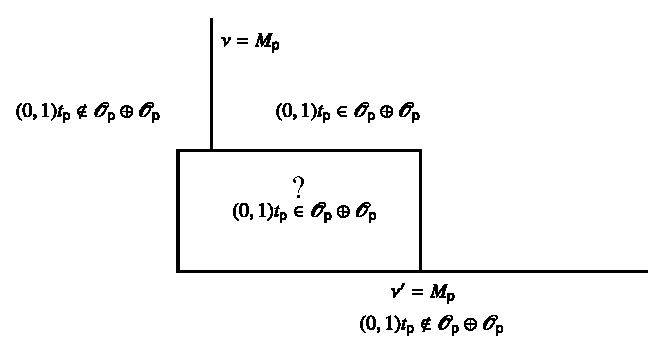
\includegraphics{chap2/fig1.eps}
\end{figure}
So\pageoriginale if $\nu\geq M_{\sfp}$ or $\nu'\geq M'_{\sfp}$ then $(0,1)t_{\sfp}\in \mathscr{O}_{\sfp}\oplus \mathscr{O}_{\sfp}$ depends only on the degree. Let us call the finite set of points described in (ii) simply $S_{\sfp}$.

If we have a regular embedding the situation becomes nicer. In this case we write $(0,1)=\alpha e_{1}+\beta e_{2}$ with $\alpha$, $\beta\in \mathscr{O}_{\sfp}$ and if we put $+M_{\sfp}=-\ord_{\sfp} (\alpha)$, $+M'_{\sfp}=-\ord_{\sfp}(\beta)$ then $(0,1)t_{\sfp}\in \mathscr{O}_{\sfp}\oplus \mathscr{O}_{\sfp}$ if and only if we have for $\deg (t_{\sfp})=(\nu,\nu')$ that $\nu\geq M_{\sfp}$ and $\nu'\geq M'_{\sfp}$. We call the embedding {\em strongly regular} if $\ord_{\sfp}(\alpha)=\ord_{\sfp}(\beta)=0$, this is the nicest case, we have $(0,1)t_{\sfp}\in \mathscr{O}_{\sfp}\oplus \mathscr{O}_{\sfp}$ if and only if $\nu$, $\nu'\geq 0$.

Now we can evaluate our integral and we write
\begin{gather*}
\int\limits_{E^{x}_{\sfp}}\Phi[(0,1)t_{\sfp}]|\det t_{\sfp}|_{\sfp}^{\frac{1}{2}+\frac{s}{2}}\widetilde{\phi}(\det t_{\sfp})\chi(t_{\sfp})d^{x}t_{\sfp}=\\[4pt]
\sum\limits^{\infty}_{\nu,\nu'=-\infty}\int\limits_{\deg(t_{\sfp})=(\nu,\nu')}\Phi[(0,1)t_{\sfp}]|\det t_{\sfp}|_{\sfp}^{\frac{1}{2}+\frac{s}{2}}\widetilde{\phi}(\det t_{\sfp})\chi(t_{\sfp})d^{x}t_{\sfp}=\\[4pt]
\sum\limits^{\nu,\nu'= +\infty}_{\nu,\nu'=-\infty}|\pi_{\sfp}|^{\left(\frac{1}{2}+\frac{s}{2}\right)(\nu+\nu')}\widetilde{\phi}(\pi_{\sfp})^{\nu+\nu'}\cdot \chi(\Pi_{\sfp})^{\nu}\cdot \chi(\Pi_{\sfp'})^{\nu'}\times\\[4pt]
\int\limits_{\sfU_{\sfp}}\Phi[(0,1)(\Pi^{\nu}_{\sfp}, \Pi^{\nu'}_{\sfp'})\epsilon]\phi(\det(\epsilon))\chi(\epsilon)d^{x}\epsilon\tag{3.1.3.3}\label{art2-eq3.1.3.3}
\end{gather*}
Now we should distinguish several cases :
\begin{itemize}
\item[$(\alpha)$] $\sfp\neq\sfp_{o}$ and $\chi$ is unramified. Then our considerations above tells us that our sum decomposes
$$
\sum\limits_{(\nu,\nu')\in S}+\sum\limits_{\substack{\nu\geq M_{\sfp}\\ N_{\sfp}\leq \nu'\leq M'_{\sfp^{-1}}}}+\sum\limits_{\substack{\nu'\geq M'_{\sfp}\\ N_{\sfp}\leq \nu'\leq M'_{\sfp^{-1}}}}+\sum\limits_{\substack{\nu\geq M_{\sfp}\\ \nu'\geq M'_{\sfp}}}
$$
The first sum is finite and in the other sums the value of the integral is always equal to $\vol_{d^{x}t_{\sfp}}(\sfU_{\sfp})$. Then these sums can be evaluated easily and we get
\begin{align*}
& G_{\sfp}(\widetilde{\phi},\psi,\chi,\gamma,s)\times{}\\
&\qquad {}\times \dfrac{(1-\widetilde{\phi}(\pi_{\sfp})^{2}\cdot |\pi_{\sfp}|^{1+s}_{\sfp})}{\left(1-\chi(\Pi_{\sfp})\widetilde{\phi}(\pi_{\sfP})|\Pi_{\sfP}|^{\frac{1}{2}+\frac{s}{2}}_{\sfP}\right)\left(1-\chi(\Pi_{\sfP})\widetilde{\phi}(\pi_{\sfP})|\Pi_{\sfP}|^{\frac{1}{2}+\frac{s}{2}}_{\sfP}\right)}
\end{align*}
where\pageoriginale we recall that $|\Pi_{\sfP}|_{\sfP}=|\Pi_{\sfP'}|_{\sfP'}=|\pi_{\sfP}|_{\sfP}$ and the numerator stems from the normalization of the characteristic function.

If our embedding is regular then we have
{\fontsize{10}{12}\selectfont
$$
G_{\sfP}(\widetilde{\phi},\psi,\chi,\gamma,s)=|\pi_{\sfP}|^{\left(\frac{1}{2}+\frac{s}{2}\right)(M_{\sfP}+M_{\sfP'})}\widetilde{\phi}(\pi_{\sfP})^{M_{\sfP}+M_{\sfP'}}\cdot \chi (\Pi_{\sfP})^{M_{\sfP}}\chi(\Pi_{\sfP'})^{M_{\sfP}}
$$}\relax
so we get an exponential factor in this case. It is equal to one in case of a strongly regular embedding.

\item[$(beta)$] $\sfp\neq \sfp_{o}$ and $\chi$ is ramified. Our character $\widetilde{\phi}$ is unramified in this case and it is clear that $\chi$ has to be ramified at $\sfP$ and $\sfP'$ since it is one on I. Therefore most of the integrals disappear and we are left with a finite sum, which gives us the desired elementary factor. In this case we can't have a regular embedding because of the earlier remark.

\item[$(\gamma)$] $\sfP=\sfP_{o}$. In this case we have in addition that $\Phi$ vanishes on $(\mathscr{O}_{\sfP}\oplus \mathscr{O}_{\sfP})\pi_{\sfP}$ and transforms under scalar multiplication as follows
$$
\Phi[\lambda(x,y)]=\overline{\phi^{2}(\lambda)}\Phi(x,y)
$$ 
If we restrict to a specific degree $(\nu\nu')$ we see that
\begin{itemize}
\item[(i)] $\Phi[(0,1)(\Pi^{\nu}_{\sfP},\Pi^{\nu'}_{\sfP'})\epsilon]=0$\qquad if $\nu$ and $\nu'$ are large.

\item[(ii)] If $\nu$ is large and $\epsilon=(\epsilon_{\sfP},\epsilon_{\sfP'})$
$$
\Phi[(0,1)(\Pi^{\nu}_{\sfP},\Pi^{\nu'}_{\sfP'})\epsilon]=\overline{\widetilde{\phi}^{2}(\epsilon_{\sfP'})}\Phi[(0,1)(\Pi^{\nu}_{\sfP},\Pi^{\nu'}_{\sfP})]
$$

\item[(ii)$'$] If $\nu'$ is large then we have
$$
\Phi[(0,1)(\Pi^{\nu}_{\sfP},\Pi^{\nu'}_{\sfP'})\epsilon]=\overline{\widetilde{\phi}^{2}(\epsilon_{\sfP})}\Phi[(0,1)(\Pi^{\nu}_{\sfP} \ \Pi^{\nu'}_{\sfP'})]
$$
\end{itemize}
\end{itemize}

If we decompose our integral according to degree we find \eqref{art2-eq2.1.3.3}
$$
\sum\limits_{\nu,\nu'\text{~small}}+\sum\limits_{\substack{\nu\text{~small}\\ \nu'\text{~large}}}+\sum\limits_{\nu\text{~large}\\ \nu'\text{~small}}
$$
where the first sum is finite. Let us consider a term
$$
\int\limits_{\sfU_{\sfP}}\Phi[(0,1)(\Pi^{\nu}_{\sfP},\Pi^{\nu}_{\sfP'})\epsilon]\widetilde{\phi}(\det \epsilon)\cdot \chi(\epsilon)d^{x}\epsilon
$$
where\pageoriginale $\nu$ is large. We have $\sfU_{\sfP}=\sfU_{\sfP}\times \sfU_{\sfP'}$, and get
$$
\int\limits_{\sfU_{\sfP}}\int\limits_{\sfU_{\sfP'}}\Phi[(0,1)(\Pi^{\nu}_{\sfP},\Pi^{\nu}_{\sfP'})]\widetilde{\phi}(\epsilon_{\sfP}/\epsilon_{\sfP'})\chi(\epsilon_{\sfP})\chi(\epsilon_{\sfP'})d^{x}\epsilon_{\sfP}d^{x}\epsilon_{\sfP'}
$$
Here we should be careful enough to say that of course
\begin{align*}
\chi(\epsilon_{\sfP})=\chi(1,\ldots, & \epsilon_{\sfP},1,\ldots)=\chi_{\sfP}(\epsilon_{\sfP})\\
                                    &\uparrow\\
                                    &\sfP\text{-th component}\\[5pt]
\chi(\epsilon_{\sfP'})=\chi(1,\ldots,1, &\epsilon_{\sfP'},1,\ldots 1)=\chi_{\sfP},(\epsilon_{\sfP'})\\
                                      &\uparrow\\
                                      &\sfP'\text{-th component}
\end{align*}
and then the condition $\chi|I_{F}=1$ implies $\chi_{\sfP}(\epsilon)=\chi_{\sfP'}(\epsilon)$ for $\epsilon \in \sfU_{\sfP}\subset F^{x}_{\sfP}$. Therefore our integral turns out to be
$$
\int\limits_{\sfU_{\sfP}}\int\limits_{\sfU_{\sfP'}}\Phi[(0,1)(\Pi^{\nu}_{\sfP},\Pi^{\nu}_{\sfP})]\widetilde{\phi}(\eta)\chi_{\sfP}(\eta)d^{x}\eta d^{x}\epsilon
$$
This integral vanishes if $\widetilde{\phi}\chi_{\sfP}$ is non trivial on $\sfU_{\sfP}\subset F^{x}_{\sfP}$. But if $\widetilde{\phi}\chi_{\sfP}$ is trivial on $\sfU_{\sfP}$ then the value of the integral is equal to
$$
\vol_{d^{x}\epsilon}(\sfU_{\sfP})\cdot \Phi[(0,1)(\Pi^{\nu}_{\sfP} \ \Pi^{\nu}_{\sfP'})]
$$
and it is clear that this value does not depend on $\nu$ but only on $\nu'$ provided $\nu$ is large.

A similar assertion holds if $\nu'$ is large. Now we interpret our conditions on $\chi_{\sfP}\cdot \widetilde{\phi}$ and $\chi_{\sfP'}\cdot \phi$ to be trivial or non trivial on $\sfU_{\sfP}$ resp. $\sfU_{\sfP'}$. Of course we have $\chi_{\sfP}\cdot \widetilde{\phi}$ is trivial on $\sfU_{\sfP}$ if and only if the character $\chi\widetilde{\phi}\circ N$ is unramified at $\sfP$ and the same holds for $\sfP'$. And we observe that $\chi\widetilde{\phi}\circ N$ can be unramified at most one of these place. Therefore we get:

If $\chi\widetilde{\phi}\circ N$ is ramified at $\sfP$ and at $\sfP'$ then in our decomposition
$$
\sum\limits_{\nu,\nu'\text{~small}}-\sum\limits_{\substack{\nu\text{~large}\\ \nu'\text{~small}}}+\sum\limits_{\substack{\nu\text{~small}\\ \nu'\text{~large}}}
$$
the second and third terms contribute zero. Then our integral is given by the first sum which is an elementary factor if $\psi$ takes values in $R$. If $\chi\widetilde{\phi}\circ N$\pageoriginale is unramified at $\sfP$ then we get a contribution from the second sum and this gives obviously again
$$
G_{\sfp}(\widetilde{\phi},\psi,\chi,\gamma,s)\frac{1}{1-\chi\widetilde{\phi}\circ N(\Pi_{\sfP})|\Pi_{\sfP'}|^{\frac{1}{2}+\frac{s}{2}}_{\sfP}}
$$
and this is again the term we want.

The same thing happens at $\sfP'$, if $\chi\widetilde{\phi}\circ N$ turns out to be unramified at $\sfP'$.

Now we discuss the case of a regular embedding and we want to give explicit expressions for the elementary factor. We write
$$
(0,1)=\alpha e_{1}+\beta e_{2}
$$
and we put $\ord_{\sfp}(\alpha)=-M_{\sfp}$, $\ord_{\sfp}(\beta)=-M'_{\sfp}$. One of these two numbers has to be zero, if both are zero then we are in the case of a strongly regular embedding.

We recall
$$
\overline{G}=\PGL_{2}(\mathscr{O}/\sfP)=\sfK^{f}/\sfK^{f}(\sfP)
$$
and we recall from \ref{art2-sec1.2.2}.
\begin{align*}
& M_{\phi}=\{\psi:\overline{G}\to R|\psi(\overline{g}\overline{b}^{-1})=\phi(\overline{b})\psi(\overline{g})\}=\\
&\left\{
\begin{array}{r}
\psi : \sfK^{f}/\sfK^{f}(\sfP)\to R|\psi(\underline{b}^{f}\underline{k}^{f})=\widetilde{\phi}(\underline{b}^{f})\cdot \psi(\underline{k}^{f})\\[4pt]
\text{for all~ } \underline{b}^{f}\in B_{o}(\bA^{f})\cap \sfK^{f}
\end{array}
\right\}
\end{align*}
(\ref{art2-lem1.6.2}) Moreover we identified the two spaces
$$
\{\Phi:\mathscr{O}/\sfP\oplus /\sfp\to R|\Phi[\lambda(x,y)]=\widetilde{\phi}^{2}(\lambda)\Phi[(x,y)]\}
$$
and $M_{\phi}$ by \eqref{art2-eq3.1.3.2}
$$
\psi(\underline{k}^{f})=\Phi[(0,1)k^{f}_{\sfp}]\cdot \widetilde{\phi}(\det k^{f}_{\sfp})
$$
Now our infinite sum over $\nu$, $\nu'$ specializes to 
$$
\text{one term for~ } \nu=M_{\sfp}, \nu'=M_{\sfp'}+\sum\limits_{\substack{\nu=M_{\sfp}\\ \nu'>M'_{\sfp}}}+\sum\limits_{\substack{\nu>M_{\sfp}\\ \nu'=M'_{\sfp}}}
$$
We\pageoriginale choose a uniformizing element $\pi_{\sfp}$ at $\sfP$ and choose $\Pi_{\sfP}$, $\Pi_{\sfP'}$ to be the projections of $\pi_{\sfp}$ to the components in $E\otimes F_{\sfp}=E_{\sfP}\oplus E_{\sfp'}$.

Then the first term is equal to
\begin{gather*}
|\pi_{\sfp}|^{\left(\frac{1}{2}+\frac{s}{2}\right)(M_{\sfp}+M'_{\sfp})}\widetilde{\phi}(\pi_{\sfp})^{M_{\sfp}+M'_{\sfp}}\chi(\Pi_{\sfP})^{M_{\sfp}}\cdot \chi(\Pi_{\sfp'})^{M_{\sfp'}}\\[4pt]
\int\limits_{\sfU_{\sfp}}\Phi[(0,1)(\Pi^{M_{\sfp}}_{\sfP},\Pi^{M_{\sfp}}_{\sfP'})\epsilon]\widetilde{\phi}(\det (\epsilon))\chi(\epsilon)d^{x}\epsilon
\end{gather*}
The vector $\xi_{o}=(0,1)(\Pi^{M_{\sfp}},_{\sfP},\Pi^{M'}_{\sfP'})=\alpha'e_{1}+\beta'e_{2}$ has both components $\alpha'$, $\beta'\neq 0$. We choose an element $k_{o}\in \sfK_{\sfp}$ with $\det (k_{o})=1$ such that $(0,1)k_{o}=\xi_{o}$. Then our integral becomes in view of \eqref{art2-eq3.1.3.2}
$$
\int\limits_{\sfU_{\sfp}}\psi(k_{o}\epsilon)\chi(\epsilon)d^{x}\epsilon=(p-1)P^{\overline{\chi}}\psi(k_{o})
$$
Here $P^{\overline{\chi}}$ is the following projection operator: The basis $e_{1}$, $e_{2}$ defines a torus $\widetilde{T}_{\gamma}\times F_{\sfp}\subset \GL_{2}/F_{\sfp}$ and the image of $\widetilde{T}_{\gamma}\times F_{\sfp}$ in $\PGL_{2}\times F_{\sfp}$ is $T_{\gamma}\times F_{\sfp}$. Let $\overline{T}_{\gamma}$ be the reduction of $T_{\gamma}\mod \sfp$. Then this is a split torus in $G$ defined by the reduction of the basis $e_{1}$, $e_{2}\mod\sfp$. Our character $\chi$ can be considered as a character on the group $\widetilde{T}_{\gamma}$ because it vanishes by assumption on the center. Then we define
$$
M^{\overline{\chi}}_{\phi}=
\left.
\begin{array}{c}
\psi\in M_{\phi}|\psi(\overline{g}\overline{t})=\phi(\overline{g})\chi(\overline{t})^{-1}\\[4pt]
\text{for~ } \overline{t}\in \overline{T}_{\gamma}
\end{array}
\right\}
$$
and $P^{\overline{\chi}}$ is the projection from $M_{\phi}$ to $M^{\overline{\chi}}_{\phi}$. We get the factor $p-1$ in front because of the normalization of the measures.

The other terms vanish by the same argument as before unless $\chi\widetilde{\phi}\circ N$ is unramified at $\sfP$ or at $\sfP'$. If for instance it is unramified at $\sfP$ we have to consider
\begin{gather*}
\int\limits_{\sfU_{\sfp}}\Phi[(0,1)(\Pi^{\nu}_{\sfp},\Pi^{M'_{\sfp'}}_{\sfp'})(\epsilon_{\sfp},\epsilon'_{\sfp})]\times{}\\
\widetilde{\phi}(\epsilon_{\sfp}\epsilon_{\sfp'})\chi_{\sfp}(\epsilon_{\sfp})\chi_{\sfp'}(\epsilon_{\sfp'})d^{x}\epsilon_{\sfp}d^{x}\epsilon_{\sfp'},
\end{gather*}
for $\nu>M_{\sfp}$. And as before we find the value for this integral is
$$
(p-1)\Phi[(0,1)(\Pi^{\nu}_{\sfp},\Pi^{M_{\sfp}}_{\sfP'})]=\Phi[e_{2}](p-1)
$$
If we treat the integral the same way we did before in the case $\nu=M_{\sfp}$, $\nu'=M'_{\sfp}$ we get : If $k_{1}\in\sfK_{\sfp}$, such that $\det(k_{1})=1$ and $(0,1)k_{1}=e_{2}$ then the integral turns out to be
$$
(p-1)P^{\widetilde{\chi}}\psi(k_{1})=(p-1)\psi(k_{1})=\Phi[e_{2}].
$$\pageoriginale
Therefore we find: If we put
$$
W_{\sfp}(\phi,\chi,s)=|\pi_{\sfp}|^{\left(\frac{1}{2}+\frac{s}{2}\right)(M_{\sfP}+M'_{\sfP})}\widetilde{\phi}(\pi_{\sfp})^{M_{\sfP}+M'_{\sfP}}\chi(\Pi_{\sfP})^{M_{\sfP}}\chi(\Pi_{\sfP'})^{M'_{\sfP}}
$$
then the value of the local contribution is equal to
\begin{align*}
& (p-1)W_{\sfp}(\phi,\psi,s)\cdot P^{\chi}\psi(k_{o})\\
&\qquad \text{if $\chi\cdot \phi\circ N$ is ramified at $\sfP$ and $\sfP'$}\\
& (p-1)\dfrac{W_{\sfp}(\phi,\chi,s)\cdot (P^{\overline{\chi}}\psi(k_{o})+\widetilde{\phi}(\pi_{\sfp})\chi(\Pi_{\sfp})|\pi_{\sfp}|^{\frac{1}{2}+\frac{s}{2}}(P^{\overline{\chi}}\psi(k_{o})-P^{\overline{\chi}}(k_{o})}{(1-\widetilde{\phi}(\pi_{\sfp})\chi(\Pi_{\sfp})|\pi_{\sfp}|^{\frac{1}{2}+\frac{s}{2}}_{\sfp}}\\
&\qquad \text{if $\chi\cdot \widetilde{\phi}\circ N$ is unramified at $\sfP$}\tag{3.1.3.2}\label{art2-eq3.1.3.2}
\end{align*}
and we get a corresponding expression in case of non ramification at $\sfP'$.

\begin{remark*}
In the first case the expression $W_{\sfp}$ does depend on the choice of $\pi_{\sfp}$ but the second factor does so too and the two factors cancel. We did all this since we want to know whether this elementary factor may vanish at $s=0$. We ignore the exponential factor and therefore we have to look at the expressions
\begin{align*}
& P^{\overline{\chi}}\psi(k_{o})\qquad \text{if $\chi\cdot \phi\circ$ Nisramified at $\sfP$ and $\sfP'$.}\\
& P^{\overline{\chi}}\psi(k_{o})+\widetilde{\phi}(\pi_{\sfp})\chi(\Pi_{\sfp})|\pi_{\sfp}|^{\frac{1}{2}}_{\sfp}(P^{\overline{\chi}}\psi(k_{1})-P^{\overline{\chi}}\psi(k_{o}))
\end{align*}
if $\chi\cdot \widetilde{\phi}\circ N$ is unramified at $\sfP$. This means that $\chi$ considered as a character on $(\mathscr{O}/\sfP)^{x}$ is equal to $\phi^{\pm 1}$. The group $\overline{T}_{\gamma}$ acts on the projective line $\overline{B}_{o}\backslash \overline{G}$ and we have exactly two fixed points therefore we get an orbit decomposition
$$
\overline{G}=\overline{B}_{o}g_{o}\cdot \overline{T}_{\gamma}\cup B_{o}x_{1}\cup B_{o}x_{2}
$$
Here we have to choose for $g_{o}$ and element in $\overline{G}$ which does not conjugate $T_{\gamma}$ into $B_{o}$ and $x_{1}$, $x_{2}$ do conjugate $\overline{T}_{\gamma}$ into $\overline{B}_{o}$.
\end{remark*}

We observe that we can for instance choose $\overline{g}_{o}$ simply the reduction of $k_{o}\mod \sfp$ and the reduction of $k_{1}$ will be $x_{1}$ or $x_{2}\mod \overline{B}_{o}$. Therefore we find if $\chi\neq \phi^{\pm 1}$
$$
M^{\overline{\chi}}_{\phi}=\{h:G\to R|h(\overline{b}\overline{g}_{o}\cdot \overline{t})=\phi(\overline{b})\cdot \chi(\overline{t})^{\pm 1}h|Bx_{1}=0,h\cdot Bx_{2}=0\}
$$
and\pageoriginale we get.

If $P^{\overline{\chi}}\psi\neq 0$ then $P^{\overline{chi}}\psi(k_{o})\neq 0$ and we know exactly when our local elementary factor does not vanish.

If $\chi=\phi^{\pm 1}$ then $\dim M^{\chi}_{\phi}=2$ and we find a basis for $M^{\overline{\chi}}_{\phi}$ by constructing $h_{1}$
$$
h_{1}(\overline{b}\overline{g}_{o}\overline{t})=\phi(\overline{b})\cdot \chi^{-1}(\overline{t})
$$
and $h_{2}\neq 0$ concentrated on $Bx_{1}$ or $Bx_{2}$. Then we have
\begin{align*}
h_{1}(k_{o})\neq 0,\quad h_{1}(k_{1})=0\\
h_{2}(k_{o})=0,\quad h_{2}(k_{1})\neq 0
\end{align*}
and again we see that for suitable $\psi\in M^{\overline{\chi}}_{\phi}$ the local expression will not be zero, for instance we can choose $\psi=\lambda h_{2}$ with $\lambda\neq 0$ and then the local factor is $\neq 0$.

\medskip
\noindent
{\em Case \thnum{II}.\label{art2-caseII}}~We assume that $E$ is non split at $\sfp$. We keep the notation $E_{\sfp}=E\otimes F_{\sfp}$ and we choose a uniformizing element $\Pi_{\sfp}$ in $E_{\sfp}$.

Then we can find two constants $M_{1}<N_{1}$ such that for $t_{\sfp}=\epsilon \cdot \Pi^{\nu}_{\sfp}$ we have
\begin{align*}
(0,1)t_{\sfp}\not\in \mathscr{O}_{\sfp}\oplus \mathscr{O}_{\sfp}\quad \text{if~ } \nu<M_{1}\\
(0,1)t_{\sfp}\in \mathscr{O}_{\sfp}\oplus \mathscr{O}_{\sfp}\quad \text{if~ }\nu>N_{1}
\end{align*}
The local contribution is equal to
\begin{gather*}
\sum\limits^{\infty}_{\nu=M_{1}}|\det \Pi_{\sfP}|^{(\frac{1}{2}+\frac{s}{2})\nu}\widetilde{\phi}(\det \Pi_{\sfP})^{\nu}\cdot \chi(\Pi_{\sfP})^{\nu}\\[4pt]
\int\limits_{\sfU_{\sfp}}\Phi[(0,1)\Pi^{\nu}_{\sfP}\epsilon]\widetilde{\phi}(\det \epsilon)\chi(\epsilon)d^{x}\epsilon
\end{gather*}
Then it is obvious that this local factor is of the form (*). We simply have to observe that for $\sfp\neq \sfp_{o}$ the integral does not depend on $\epsilon$ if $\nu<N_{1}$. If $\sfp=\sfp_{o}$ then the function $\Phi[(0,1)\pi^{\nu}_{\sfp}\epsilon]=0$ if $\nu$ is large and we get a finite sum. Here we have to take into account that the character $\phi$ is ramified at $\sfp_{o}$ and that in this case $\chi\cdot \phi\circ N$ is ramified at $\sfP$.

Again we discuss the case of a regular embedding more closely 
\begin{itemize}
\item[$(\alpha)$] $\sfp\neq \sfp_{o}$ and $E/F$ is unramified at $\sfp$. Then we choose of course $\Pi_{\sfp}=\pi_{\sfp}$ and we have $\sfU_{\sfp}=E^{x}_{\sfp}\cap \GL_{2}(\mathscr{O}_{\sfp})$. Then for $t_{\sfp}=(0,1)\pi^{\nu}\epsilon \in \mathscr{O}_{\sfp}\oplus \mathscr{O}_{\sfp}$ if and only if $\nu\geq 0$. We recall that it follows from our assumptions that $\chi|\sfU_{\sfp}=1$,\pageoriginale only these $\chi$ are of interest for us. Then the local factor is equal to
$$
\frac{1-\widetilde{\phi}\circ N(\pi_{\sfp})\cdot \chi(\pi_{\sfp})|\det \pi_{\sfp}|^{\frac{1}{2}+\frac{s}{2}}_{\sfp}}{1-\widetilde{\phi}^{2}(\pi_{\sfp})|\pi_{\sfp}|^{1+s}}=1
$$

\item[$(\beta)$] The extension is ramified at $\sfp$. We may have two cases, namely
$$
(0,1)\Pi^{\nu}_{\sfP}\epsilon \in \mathscr{O}_{\sfp}\oplus \mathscr{O}_{\sfp}\qquad \text{if and only if~ } \nu\geq -1
$$
or
$$
(0,1)\Pi^{\nu}_{\sfP}\epsilon \in \mathscr{O}_{\sfp}\oplus \mathscr{O}_{\sfp}\qquad \text{if and only if~ }\nu\geq 0.
$$
If $M_{o}=-1$ in the first case and $M_{o}=0$ in the second case, we find as local contribution
\begin{gather*}
\sum\limits^{\infty}_{\nu=M_{o}}|\det \Pi_{\sfP}|^{\left(\frac{1}{2}+\frac{s}{2}\right)\nu}_{\sfp}\cdot \widetilde{\phi}(\det \Pi_{\sfP})^{\nu}\cdot \chi(\Pi_{\sfP})^{\nu}\cdot \\[4pt]
\int\limits_{\sfU_{\sfp}}\Phi[(0,1)\pi^{\nu}_{\sfp}\epsilon]\widetilde{\phi}(\det \epsilon)\chi(\epsilon)d^{x}\epsilon
\end{gather*}
The function under the integral sign is constant since $\widetilde{\phi}$ and $\chi$ are unramified. We map $\sfU_{\sfp}$ into $E^{x}_{\sfp}/F^{x}_{\sfp}$ then the image is of index 2. Since we normalized vol $(E^{x}_{\sfp}/F^{x}_{\sfp})=1$ we get as local contribution
\begin{multline*}
\frac{1}{2}|\det \Pi_{\sfp}|^{\left(\frac{1}{2}+\frac{s}{2}\right)M_{o}}_{\sfp}\widetilde{\phi}(N(\Pi_{\sfp}))^{M_{o}}\cdot \chi(\Pi_{\sfp})^{M_{o}}\\
\frac{1-\widetilde{\phi}^{2}(\pi_{\sfp})|\pi_{\sfp}|^{1+s}}{1-\chi(\Pi_{\sfP})\widetilde{\phi}(N(\Pi_{\sfP}))|\Pi_{\sfP}|^{\frac{1}{2}+\frac{s}{2}}_{\sfP}}
\end{multline*}
and the elementary factor is exponential.

\item[$(\gamma)$] $\sfp\neq \sfp_{o}$ and the extension is unramified at $\sfp$. This is the nicest case the local integral is equal to
$$
\int\limits_{\sfU_{\sfp}}\Phi[(0,1)\epsilon]\widetilde{\phi}^{2}(\det\epsilon)\chi(\epsilon)d^{*}\epsilon=(p+1)\cdot P^{\overline{\chi}}\psi(1)
$$
Here we observe that the reduction mod $\sfp$ of $T_{\gamma}$ is an anisotropic torus $\overline{T}_{\gamma}$ in $\overline{G}$ and $\overline{P}$ is the projection to the space
$$
M^{\overline{\chi}}_{\phi}=\{\psi:G\to R|\psi(\overline{b}\overline{g}\overline{t})=\phi(\overline{b})\psi(\overline{g})\chi(\overline{t})^{-1}\text{~ for~ } \overline{b}\epsilon \overline{B}_{o},\overline{t}\in \overline{T}_{\gamma}\}
$$
Since $\overline{G}=\overline{B}_{o}\overline{T}_{\gamma}$ this space is of dimension 1 and generated by a function $\psi_{1}$ which satisfies $\psi_{1}(1)=1$, the local factor is $\neq 0$.

\item[$(\delta)$] $\sfp=\sfp_{o}$\pageoriginale and the extension $E/F$ is ramified at the place $\sfp$. The group of units injects into $\GL_{2}(\mathscr{O}_{\sfp})$ and this induces an injection
$$
\sfU_{\sfp}/\sfU_{\sfp}^{(2)}\hookrightarrow \GL_{2}((\mathscr{O}/\sfp))
$$
where $\sfU^{(2)}_{\sfp}=\{\epsilon|\epsilon\equiv 1\mod \sfP^{2}\}$. The units of $F_{\sfp}$ mapped into $\GL_{2}(\mathscr{O}/\sfp)$ fill up the center and we get
$$
\overline{T}_{\gamma}=\iIm(\sfU_{\sfp}/\sfU_{\sfp}^{(2)}\to \overline{G})
$$
is cyclic of order $p$, this means that $T_{\gamma}$ is the group of $\mathscr{O}/\sfp$-valued points of a Borel subgroup of $\overline{G}$. The element $\pi_{\sfp}$ induces via multiplication an endomorphism of $\mathscr{O}_{\sfp}\oplus \mathscr{O}_{\sfp}$. The reduction of this endomorphism to $\mathscr{O}/\sfp\oplus \mathscr{O}/\sfp$ has obviously a one dimensional kernel, which is generated by a vector $\xi_{1}\epsilon \mathscr{O}_{\sfp}\oplus \mathscr{O}_{\sfp}$. It is clear that the reduction of $\xi_{1}\mod \sfp$ generates the stabilizer of $\overline{T}_{\gamma}$. This tells us that we have to consider two cases
\begin{align*}
& \delta 1)\overline{T}_{\gamma}\subset \overline{B}_{o}\langle =\rangle (0,1)\Pi^{-1}_{\sfp}\in \mathscr{O}_{\sfp}\oplus \mathscr{O}_{\sfp}\\
& \delta 2)\overline{T}_{\gamma}\nsubset \overline{B}_{o}\langle =\rangle (0,1)\Pi^{-1}_{\sfp}\in \mathscr{O}_{\sfp}\oplus \mathscr{O}_{\sfp}
\end{align*}
In the case $\delta)$ we get the local contribution
\begin{gather*}
|\det \Pi_{\sfP}|^{-\left(\frac{1}{2}+\frac{s}{2}\right)}_{\sfP}\widetilde{\phi}(\det\Pi_{\sfP})^{-1}\chi(\Pi_{\sfP})^{-1}\cdot\\
\int\limits_{\sfU_{\sfp}}\Phi[(0,1)\pi^{-1}_{\sfp}\epsilon]\widetilde{\phi}(\det \epsilon)\cdot \chi(\epsilon)d^{x}\epsilon+{}\\
{}+ \int\limits_{\sfU_{\sfp}}\widetilde{\Phi}[(0,1)\epsilon]\widetilde{\phi}(\det \epsilon)\chi(\epsilon)d^{x}\epsilon
\end{gather*}
Now the situation is quite similar to the split case. We choose $k_{o}\in \sfK_{\sfp}$ with $\det(k_{o})=1$ such that $(0,1)\pi^{-1}_{\sfP}=(0,1)k_{o}$ then we get
$$
\frac{\pi}{2}(|\Pi_{\sfP}|^{\frac{1}{2}+\frac{s}{2}}_{\sfP}\widetilde{\Phi}(N(\Pi_{\sfP}))^{-1}\chi(\Pi_{\sfP})^{-1}P^{\overline{\chi}}\psi(k_{o})+P^{\chi}\psi(1))
$$
The vector $(0,1)\Pi^{-1}_{\sfp}\mod \sfp$ is not stabilized by $\overline{B}_{o}$ and therefore the image $\overline{k}_{o}$ of $k_{o}$ in $\overline{G}$ is not contained in $\overline{B}_{o}$. We have
$$
\overline{G}=\overline{B}_{o}\cdot \overline{k}_{o}\cdot \overline{T}_{\gamma}\cup \overline{B}_{o}
$$
and we get that $\dim M^{\overline{\chi}}_{\phi}=1$ (resp. 2) if $\overline{\chi}\neq 1$ (resp $\overline{\chi}=1$). In both cases we can construct a $\psi\in M^{\overline{\chi}}_{\phi}$ such that $\psi(k_{o})\neq 0$ and $\psi(1)=0$, and this implies that with this choice the elementary factor is non zero.

The\pageoriginale case $\delta 2)$ is quite similar. In this case we have also to sum over two terms namely $(0,1)\epsilon$, $(0,1)\Pi_{\sfp}\epsilon$. Then we get
$$
\frac{p}{2}P^{\overline{\chi}}\psi(1)+|\Pi_{\sfP}|^{\frac{1}{2}+\sfrac{s}{s}}_{\sfP}\widetilde{\phi}(N(\Pi_{\sfP}))\cdot \chi(\Pi_{\sfP})P^{\overline{\chi}}\psi(k_{1}))
$$
where $(0,1)\pi_{\sfP}=(0,1)k_{1}$. The same argument as above shows the non vanishing if $\psi$ is suitably chosen.
\end{itemize}

\subsubsection{The Infinite Place}\label{art2-sec3.1.5}
We have to evaluate the integral
$$
\int\limits_{T_{\gamma}(\mathbb{C})}\omega^{(\infty)}_{s}(t_{\infty}g_{\gamma},\widetilde{\phi})dj_{x_{\gamma}}(Y))d^{x}t_{\infty}
$$
We recall that (\ref{art2-sec1.6})
\begin{gather*}
\omega^{(\infty)}_{s}(g_{\infty},\phi)=\omega^{(\infty)}_{s}(b_{\infty}k_{\infty},\widetilde{\phi})=\\
|b_{\infty}|^{+\frac{1}{2}+\frac{s}{2}}_{\mathbb{C}}\widetilde{\phi}(b_{\infty})(\ad k^{-1}_{\infty})\cdot e_{\epsilon(\phi)}
\end{gather*}
where $b_{\infty}=\left(\begin{smallmatrix} x_{\infty} & u\\ 0 & 1\end{smallmatrix}\right)\in B_{o}(\mathbb{C})$ and
$$
|b_{\infty}|^{\frac{1}{2}+\frac{1}{2}s}_{\mathbb{C}}\widetilde{\phi}(b_{\infty})=|x_{\infty}|_{\mathbb{C}}^{\frac{1}{2}+\frac{1}{2}s}\cdot \widetilde{\phi}(x_{\infty})
$$
We recall that $T_{\gamma}(\mathbb{C})=T^{(s)}_{\gamma} xT^{(c)}_{\gamma}=R^{x}_{+}xS^{1}$ \eqref{art2-sec3.1} and we have selected $g_{\gamma}$ in such a way that
$$
\langle \omega^{\infty}_{s}(t_{\infty}g_{\gamma},\phi),dj_{x_{\gamma}}(Y)\rangle
$$
does not depend on the circular variable. \eqref{art2-sec3.1}.

Now we have of course that $E_{\infty}=F_{\infty}\otimes E=\mathbb{C}\otimes E=\mathbb{C}\oplus \mathbb{C}$, this defines a split torus in $\PGL_{2}(\mathbb{C})$ and this torus is certainly not contained in $B_{o}(\mathbb{C})$.

We can find a matrix
$$
x=\left(\begin{matrix} y & u\\ 0 & 1\end{matrix}\right)\in B_{o}(\mathbb{C})
$$
such that
$$
T_{\gamma}(\mathbb{C})=xT_{1}x^{-1}
$$
where\pageoriginale
$$
T_{1}=\left\{\left(\begin{matrix} a & b\\ b & a\end{matrix}\right)\Big| a,b\in \mathbb{C}, a^{2}-b^{2}\neq 0\right\}\mod \text{ center of } \GL_{2}(\mathbb{C})
$$
and one checks that $y$ is unique up to a sign. The maximal compact subgroup of $T_{1}$ is contained in the maximal compact subgroup $K_{\infty}$ and therefore we can take $g_{\gamma}=x$. Our integral becomes
$$
\int\limits_{T_{1}}\langle \omega^{(\infty)}_{s}(xt_{1},\phi),\ad(x^{-1})\cdot (Y)\rangle d^{x}t_{1}
$$
The generator $Y\in \Lie (T^{(s)}_{\gamma})$ is selected in a canonical way up to a sign since the character module of the torus $T_{\gamma}$ has a canonical generator $\lambda_{o}$ up to a sign and $d\lambda(Y)=1$. Therefore we get that
$$
\ad(x^{-1})(Y)=\pm\left(\begin{matrix} 0 & 1\\ 1 & 0\end{matrix}\right)\in \sfp
$$
and we choose $y$ in such a way that
$$
\ad(x^{-1})(Y)=\left(\begin{matrix} 0 & 1\\ 1 & 0\end{matrix}\right)=E_{1}
$$
Observing that the integral does not depend on the circular variable we find for the value of the integral
$$
|y|^{\frac{1}{2}+\frac{s}{2}}_{\mathbb{C}}\widetilde{\phi}(y)\int\limits_{T_{1}^{(s)}}\langle \omega^{(\infty)}_{s}(t,\widetilde{\phi}),E_{1}\rangle d^{x}t
$$
and
\begin{align*}
T^{(s)}_{1}=\left\{\exp x\left(\begin{matrix} 0 & 1\\ 1 & 0\end{matrix}\right)\Big| x\in \IR\right\}=\\
\left\{\left(\begin{matrix} \cos hx \sin hx\\ \sin hx\cos nx\end{matrix}\right)=t(x)\Big| x\in \IR\right\}
\end{align*}
and the measure was normalized such that we have to compute
$$
|y|^{\frac{1}{2}+\frac{s}{2}}_{\mathbb{C}}\widetilde{\phi}(y)\int\limits^{+\infty}_{-\infty}\langle \omega^{(\infty)}_{s}(t(x),\widetilde{\phi}),E_{1}\rangle \dx
$$
We put $h(x)=(\cos h^{2}x+\sin h^{2}x)^{\frac{1}{2}}$ and get
$$
t(x)=\left(\begin{matrix}
h(x)^{-1} & *\\
0 & h(x)
\end{matrix}\right)
\left(\begin{matrix}
\frac{\cos hx}{h(x)} & \frac{\sin hx}{h(x)}\\[4pt]
-\frac{\sin hx}{h(x)} & \frac{\cos hx}{h(x)}
\end{matrix}\right)
=b(x)\cdot k(x)
$$
Then\pageoriginale the integral is equal to
$$
|y|^{\frac{1}{2}+\frac{s}{2}}_{\mathbb{C}}\widetilde{\phi}(y)\int\limits^{+\infty}_{-\infty}h(x)^{-2-2s}\langle \ad k(x)^{-1}e_{\epsilon(\phi)},E_{1}\rangle \dx
$$
But $\langle \ad k(x)^{-1}e_{\epsilon(\phi)},E_{1}\rangle=\langle e_{\epsilon(\phi)},\ad k(x)E_{1}\rangle$.

From \eqref{art2-eq1.4.1} we get that
$$
\langle e_{\epsilon(\phi)},\ad k(x)E_{1}\rangle =h(x)^{-2}\cdot \langle E_{1},E_{1}\rangle =h(x)^{-2}
$$
and we wind up with
$$
|y|^{\frac{1}{2}+\frac{s}{2}}_{\mathbb{C}}\widetilde{\phi}(y)\int\limits^{+\infty}_{-\infty}(\cos h^{2}x+\sin h^{2}x)^{-2-s}\dx
$$
and this integral turns out to be equal to
$$
\frac{1}{2}\cdot |y|^{\frac{1}{2}+\frac{s}{2}}_{\mathbb{C}}\cdot \widetilde{\phi}(y)\dfrac{\Gamma(s/2+1)\Gamma(1/2)}{\Gamma\left(\frac{s+1}{2}+1\right)}
$$
and if we exploit Legendre's duplication formula (\cite{art2-key28}, 12.15) we find
$$
2^{s}|y|^{\frac{1}{2}+\frac{s}{2}}_{\mathbb{C}}\widetilde{\phi}(y)\cdot \frac{\Gamma\left(\frac{s}{2}+1\right)^{2}}{\Gamma(s+2)}
$$
for the local contribution.

Now we can evaluate at $s=0$. Then the value of the integral is the value of the period of the class $[E(\phi,\psi,0)]$ on the cycle $\sum\limits_{\xi\in I_{\gamma}}\chi(\xi)z_{\gamma_{\xi}}$ and this is an intrinsic value which does not depend on the different choices we made. We get our second main theorem.

\medskip
\noindent
{\bf Theorem \thnum{3.1.6}.\label{art2-thm3.1.6}}~{\em The value of the Eisenstein class $[E(\phi,\psi,0)]$ on the cycle}
$$
\sum\limits_{\xi\in I_{\gamma}}\chi(\xi)Z_{\gamma_{\xi}}
$$
{\em for a primitive $\gamma\in \Gamma$ is given by}
$$
|y|^{\frac{1}{2}}_{\mathbb{C}}\widetilde{\Phi}(y)\cdot \Pi_{\sfp}G_{\sfp}(\widetilde{\phi},\psi,\chi,\gamma,0)\cdot \dfrac{L_{E}\left(\chi\widetilde{\phi}\circ N,\frac{1}{2}\right)}{L_{F}(\widetilde{\phi}^{2},1)}
$$
{\em We\pageoriginale have that almost all local elementary factors $G_{\sfp}(\phi,\psi,\chi,\gamma,0)=1$. If our embedding is regular at all places, then we can choose $\psi$ so that all local factors $\neq 0$.}

\begin{remark*}
The theorem as it is stated is somewhat weak because we do not say very much about the elementary factors. So we should understand it in connection with our results on these factors which have been obtained in course of the computations. It seems to be difficult to incorporate these computational results into the statement of the theorem.
\end{remark*}

\section{Arithmetic Applications}\label{art2-sec4}

In the beginning of \ref{art2-sec3.1} we stated without proof that the classes 
$$
[E(\underline{g},\phi,\psi,0)]
$$ 
are cohomology classes in $H^{1}(\Gamma\backslash X,K)$, where $K$ is the field of fraction of $R$. We want to accept this fact form now on, in any case we have given several examples in \ref{art2-sec2.2} in the cases $\sfP_{o}=(2-i)$, $\sfP_{o}=(3+2i)$ where we checked this assumption directly. We abbreviate
$$
[E(\underline{g},\phi,\psi,0)]=\Phi_{E}(\psi)
$$
and then we get a homomorphism
$$
\Phi_{E}(\psi):\Gamma\to K
$$
Then our main theorem \ref{art2-thm3.1.6} may also be stated as follows:

Let $\gamma\in \Gamma$ be primitive, let $I_{\gamma}$ the group of classes in the genus of $\gamma$, for any character $\chi:I_{\gamma}\to S^{1}$ we consider
$$
\sum\limits_{\xi\in I_{\gamma}}\chi(\xi)\gamma_{\xi}\in \Gamma/[\Gamma,\Gamma]\otimes Z[\chi]
$$
where ($Z[\chi]$ is the ring of integers of the field generated by the values of $\chi$). Then
$$
\Phi_{E}(\psi)(\sum \chi(\xi)\gamma_{\xi})=|y|_{\mathbb{C}}^{\frac{1}{2}}\widetilde{\phi}(y)\cdot \Pi_{\sfp}G_{\sfp}(\widetilde{\phi},\psi,\chi,\gamma,0)\frac{L_{E}\left(\chi\cdot \widetilde{\phi}\circ N,\frac{1}{2}\right)}{L_{F}(\widetilde{\phi}^{2},1)}
$$
The first consequence of this formula is

\medskip
\noindent
{\bf Corollary \thnum{4.1}.\label{art2-coro4.1}}~{\em The\pageoriginale number}
$$
|y|^{\frac{1}{2}}_{\mathbb{C}}\widetilde{\phi}(y)\cdot (\Pi_{\sfp}G_{\sfp}(\widetilde{\phi},\psi,\chi,\gamma,0))\frac{L_{E}\left(\chi\cdot \widetilde{\phi}\circ N,\frac{1}{2}\right)}{L_{F}(\widetilde{\phi}^{2},1)}
$$
{\em is in $K[\chi]$}
\smallskip

We have an action of the Galois group $\Gal (K(\chi)/Q)$ on the group
$$
\Hom (\Gamma,K(\chi))
$$
simply given by the action on the group of values. This induces an action of this Galois group on the characters $\phi$, $\chi$ and on the functions $\psi$. Since it follows from the above theorem, that $\Phi_{E}(\psi)^{\sigma}=\Phi(\psi^{\sigma})$ we get even information concerning the galois action on the above numbers
\begin{gather*}
\left(|y|^{\frac{1}{2}}\cdot \widetilde{\phi}(y)(\Pi_{\sfp}G_{\sfp}(\widetilde{\phi},\psi,\chi,\gamma,0))\frac{L_{E}\left(\chi\cdot \widetilde{\phi}\circ N,\frac{1}{2}\right)}{L(\widetilde{\phi}^{2},1)}\right)^{\sigma}=\\
|y|^{\frac{1}{2}}\widetilde{\phi}^{\sigma}(y)(\Pi_{\sfp}G_{\sfp}(\widetilde{\phi}^{\sigma},\psi^{\sigma},\chi^{\sigma},\gamma,0))\frac{L\left(\chi^{\sigma}\circ N,\frac{1}{2}\right)}{L((\widetilde{\phi}^{\sigma})^{2},1)}
\end{gather*}
But we can say a little bit more: The Eisenstein classes $\Phi_{E}(\psi):\Gamma\to K$ have of course to satisfy certain integrality conditions. This means that in any given case we find a number $d\in Z$, such that $\Phi_{E}(\psi)$ takes its values already in $R'=R\left[\chi,\frac{1}{d}\right]$. Then we get of course the same estimates for the denominators of the right hand side. In any case these questions about the denominators in the Eisenstein classes seem to be very interesting. We discussed already some of the aspects at the end of \ref{art2-sec2.2}. We should certainly expect those primes in the denominator which occur in the torsion of the cohomology of $\Gamma$. We should also expect the primes dividing $c_{\phi}$. But we can say that if there are other primes in the denominator of an Eisenstein class, then they will create congruences between the Fourier coefficients of cusp forms and Eisenstein series. We hope to come back to these questions later.

Of\pageoriginale course the main object of interest are the values $L_{E}(\chi,\widetilde{\phi}\circ N,\frac{1}{2})$ themselves. If we want to understand these values we have to get hold of the local factors, especially we have to prove that they are non zero. We have collected some informations concerning this question, but I do not want to discuss these problems in this paper. Instead of trying to give a general statement I will treat a very special example where one can see how our results can be used to get informations on these special values of $L$-functions. Before I come to this example I want to say one more word about the relationship of our result to Shimura's results in \cite{art2-key24}. He considers special values of $L$-functions $L_{E}(\eta,s)$ where $E$ is a CM field and $\eta$ a Grossencharakter of type $A_{o}$. He proves that for certain special values of $s$ the value of the $L$-function divided by a suitable power of a period is an algebraic number.

Our method here gives some information on the ratios
$$
\frac{L_{E}\left(\chi\cdot \widetilde{\phi}\circ N,\frac{1}{2}\right)}{L_{F}(\widetilde{\phi}^{2},1)}
$$
where the period $\omega^{2}$ cancels out. So our information is weaker to some extent, but we get informations for an infinite number of fields $E/\mathbb{Q}$, which are not necessarily CM-fields. We get informations on the Galois action and on the denominators. In some cases we get even an effective procedure to compute these ratios, and I want to conclude this paper by describing this procedure and doing the computation in one specific case.

We identified the space of $R$-valued function $\sfC(\overline{G})$ with the group ring
\begin{gather*}
\sfC(\overline{G})\xrightarrow{\sim}R[\overline{G}]\\
f\to \sum\limits_{\sigma\in \overline{G}}f(\sigma)\sigma
\end{gather*}
This is an isomorphism of $\overline{G}\times \overline{G}$-modules, the actions on the group ring are given by
\begin{align*}
L_{\tau}:m &= \sum\limits_{\sigma\in G}a_{\sigma}\sigma\to \sum\limits_{\sigma\in G}a_{\sigma}\tau \sigma=\sum\limits_{\sigma\in G}a_{\tau^{-1}\sigma}\sigma\\[4pt]
R_{\tau}:m &=\sum\limits_{\sigma\in G}a_{\sigma}\sigma\to \sum\limits_{\sigma\in G}a_{\sigma}\sigma \tau^{-1}=\sum\limits_{\sigma\in G}a_{\sigma\tau}\sigma
\end{align*}
We\pageoriginale consider $R[\overline{G}]$ as a $\Gamma_{o}$-module with respect to the action induced by right multiplication and with respect to this action we defined 
$$
H^{1}(\Gamma_{o},R[\overline{G}])
$$ 
and we have \eqref{art2-sec1.1}
$$
H^{1}(\Gamma_{o},R[\overline{G}]=H^{1}(\Gamma,R)
$$
In $\sfC[\overline{G}]$ we considered the submodule \eqref{art2-sec1.2.3}
$$
N_{\phi}=\{f:\overline{G}\to R|f(\overline{b}\overline{g})=\phi(\overline{b})\cdot f(\overline{g})\}
$$
and in some cases we have explicitely computed the cohomology groups \eqref{art2-sec2.2}
$$
H^{1}(\Gamma_{o},N_{\phi})\hookrightarrow H^{1}(\Gamma_{o},R[\overline{G}])
$$
In those case which we considered we found that $\dim_{R}H^{1}(\Gamma_{o},N_{\phi})=1$ and we did even better namely we constructed explicitely cocycles
$$
\Phi:\Gamma_{o}\to N_{\phi}
$$
whose cohomology class generates the cohomology. Here we observe, that such a cocycle
$$
\Phi :\Gamma_{o}\to N_{\phi}
$$
is uniquely determined by its class, provided we know that $\Phi:\Gamma_{oB_{o}}\to N_{\phi}^{\sfU_{o}}$. Therefore we can say that the cocycle $\Phi$ is a canonical representative of the given class.

Now we got from our construction \eqref{art2-sec1.2.3} that the class $\Phi$ which satisfied \eqref{art2-sec2.2}
$$
\Phi\left(\left(\begin{matrix} 1 & 1\\ 0 & 1\end{matrix}\right)\right)=\left(\sum\limits_{u\in U_{o}}\delta_{\overline{u}}\right)+b\cdot \delta_{\infty}
$$
has to be equal to the Eisenstein class, i.e.
$$
[\Phi]=[E(\phi,\psi_{o},0)]
$$
where we have $\psi_{o}\in M_{\phi}$ and 
$$
\psi_{o}(\overline{g})=
\begin{cases}
\phi(\overline{b})^{-1} & \text{for~ } \overline{g}=\overline{u}w\overline{b}\\[3pt]
0 & \text{for~ } \overline{g}=\overline{b}
\end{cases}
$$
This\pageoriginale tells us that the cocycles which we computed in the examples in \eqref{art2-sec2.2} actually are equal to the canonical representatives of a very specific Eisenstein class.

\begin{remark*}
This argument of course breaks down if we do not know that $H^{1}(\Gamma_{o},N_{\phi})$ is of rank 1. In that case we have to separate the Eisenstein class from the other classes by using the action of the Hecke algebra.
\end{remark*}

Now it is clear how we get an ``explicit'' formula for the value
$$
[E(\phi,\psi_{o},0)](\gamma)
$$
for $\gamma\in \Gamma$. Let us assume we have computed the value $\Phi(\gamma)$ of the representing cocycle on $\gamma$. Then
$$
\Phi(\gamma)=\sum\limits_{\sigma\in \overline{G}}\phi_{\sigma}(\gamma)\sigma
$$
and according to \eqref{art2-sec1.1} we have
$$
[E(\phi,\psi_{o},0)](\gamma)=\Phi_{1}(\gamma)
$$
Now we have a set of generators for $\Gamma_{o}$ namely the matrices
\begin{align*}
u(\alpha) &= \left(\begin{matrix} 1 & \alpha\\ 0 & 1\end{matrix}\right)\qquad \alpha\in \mathscr{O}\\[4pt]
B &= \left(\begin{matrix} 0 & 1\\ -1 & 0\end{matrix}\right)\quad\text{and}\quad C=\left(\begin{matrix} i & 0\\ 0 & 1\end{matrix}\right)
\end{align*}
We know in our examples the value of $\Phi$ on each of the generators and if $\gamma=\gamma_{1},\ldots,\gamma_{t}$ is written as a product of generators then we have
$$
\Phi(\gamma)=\sum\limits^{t}_{\nu=1}R\overline{\gamma_{1},\ldots,\gamma_{\nu-1}}\Phi(\gamma_{\nu})=\sum\limits^{t}_{\nu=1}\sum\limits_{\sigma\in\overline{G}}\Phi_{\sigma}\overline{\gamma_{1},\ldots,\gamma_{\nu-1}}(\gamma_{\nu})\sigma
$$
where $\overline{\gamma_{1},\ldots,\gamma_{\nu-1}}$ is the image of $\gamma_{1},\ldots,\gamma_{\nu-1}$ in $\overline{G}$. We have
$$
\Phi_{1}(\gamma)=\sum\limits^{t}_{\nu=1}\Phi\overline{\gamma_{1}\quad \gamma_{\nu-1}}(\gamma_{\nu})
$$
and if we interpret $\Phi(\gamma)\in R[\overline{G}]$ as an $R$-valued function on $\overline{G}$, then we find
$$
\Phi_{1}(\gamma)=[E(\phi,\psi_{o},0)](\gamma)=\sum\limits^{t}_{\nu=1}\Phi(\gamma_{1})\overline{(\gamma_{1},\ldots,\gamma_{\nu-1})}
$$
We\pageoriginale want to generalize this formula slightly, we are interested in 
$$
[E(\phi,\psi,0)](\gamma)\quad\text{for all}\quad \psi\in M_{\phi}.
$$ 
We observe that $M_{\phi}$ is an irreducible $\overline{G}$-module with respect to the action induced by multiplication from the left. Therefore it suffices to compute these numbers in the special case that $\psi=L_{\sigma_{o}}(\phi_{o})$ for $\sigma_{o}\in \overline{G}$. Then we get of course the representing cocycle
$$
L_{\sigma_{o}}\Phi(\gamma)=\sum\limits_{\sigma}\Phi_{\sigma}(\gamma)\sigma_{o}\sigma
$$
and form that we get the formula
\begin{equation*}
[E(\phi,L_{\sigma_{o}}\phi_{o},0)](\gamma)=\sum\limits^{t}_{\nu=1}\Phi(\gamma_{\nu})\sigma^{-1}_{o}\gamma_{1},\ldots,\gamma_{\nu-1}\tag{4.1}\label{art2-eq4.1}
\end{equation*}
if $\gamma=\gamma_{1},\ldots,\gamma_{t}$ is a presentation of $\gamma$ as a word in the generators of $\Gamma_{o}$ we gave above.

Now we want to evaluate the formula in one special case. We take $\sfP_{o}=(2-i)$ and $E/F$ shall be the field of eight roots of unity.

If $\zeta=\sqrt{i}=e^{\frac{\pi i}{4}}$ then we have
$$
\mathscr{O}_{E}=\mathscr{O}_{F}[\zeta]
$$
(\cite{art2-key12}, IV, Thm. 3). This field contains the maximal totally real subfield $L=\mathbb{Q}(\sqrt{2})$ and the fundamental unit in $L$ is $1+\sqrt{2}=\epsilon$. We embed $E\hookrightarrow M_{2}(F)$ by means of the identification
$$
a+b\zeta\to (a,b)
$$
and then we have
$$
E=\left\{\left(\begin{matrix} a & b\\ bi & a\end{matrix}\right)\Big| a,b\in F\right\}\subset M_{2}(F)
$$
Since we have $\mathscr{O}_{E}=\mathscr{O}_{F}[\zeta]$ this embedding is everywhere strongly regular as one checks easily. Now the element $\eta=\epsilon^{3}$ is a primitive element in the group $\Gamma$ and it is given by the matrix
$$
\eta=\left(\begin{matrix} 7 & 5-5i\\ 5+5i & 7\end{matrix}\right)=\gamma
$$
The class number of $E$ is one and starting from this one checks that there is only one class in the genus of $\gamma$, this is so since $(\mathscr{O}_{E}/\sfp_{o}\mathscr{O}_{E})^{x}/(\mathscr{O}_{F}/\sfp_{o})^{x}$ global units = 1. This means there is only the\pageoriginale trivial character $\chi_{o}=1$ and our main theorem says-
$$
[E(\phi,\psi,0)](\gamma)=\text{~product of local factors }\times \frac{L_{E}\left(\widetilde{\phi}\circ N,\frac{1}{2}\right)}{L_{F}(\widetilde{\phi}^{2},1)}
$$
We have to determine the local factors. They are certainly equal to one at all places except $(1-i)$, $\sfp_{o}$ and infinity. So we compute these factors explicitely at these places.

We look at $(1+i)$ first. In this case we have the uniformizing element $\pi_{2}=(1-\zeta)$. Then
$$
\pi^{-1}_{2}=\frac{1}{1-\zeta}=\frac{1+\zeta}{(1-\zeta)(1+\zeta)}=\frac{1+\zeta}{1-i}
$$
The corresponding matrix is
$$
\frac{1}{1-i}\left(\begin{matrix} 1 & 1\\ i & 1\end{matrix}\right)
$$
and
$$
(0,1)\cdot \pi^{-1}_{2}=\frac{1}{1-i}(0,1)\left(\begin{matrix} 1 & 1\\ i & 1\end{matrix}\right)=\frac{1}{1-i}(i,1)
$$
and hence $(0,1)\pi^{-1}_{2}\not\in \mathscr{O}_{2}\oplus \mathscr{O}_{2}$. We are in case II, $\beta$) and find the local elementary factor
$$
G_{2}(\widetilde{\phi},\psi_{o},\chi,\gamma,0)=\frac{1}{2}
$$
Now we look at the local factor at $\sfp=\sfp_{o}=(2-i)$. We are in case II, $\gamma$) and we have to compute
$$
(p+1)P^{\chi_{o}}\psi_{o}(1)=\sum\limits_{t\in \overline{T}_{\gamma}}\psi_{o}(t)
$$
The group $\overline{T}_{\psi}$ is cyclic of order 6 and generated by $\eta=\left(\begin{smallmatrix} 3 & 1\\ 2 & 3\end{smallmatrix}\right)$.

Recalling the definition of $\psi_{o}$ and we find
$$
G_{\sfp_{o}}(\widetilde{\phi},\psi_{o},\chi_{o},\gamma,0)=6\cdot P^{\chi_{o}}\psi_{o}(1)=2+i
$$
And\pageoriginale at infinity our torus is given by
$$
T_{\gamma}(\mathbb{C})=\left\{\left(\begin{matrix} a & b\\ bi & a\end{matrix}\right)\Big|a,b\in \mathbb{C}\right\}\Big/\text{~center}
$$
If we choose our matrix
$$
x=\left(\begin{matrix} \zeta^{-1} & 0\\ 0 & 1\end{matrix}\right)
$$
then $T_{\gamma}(\mathbb{C})=xT_{1}x^{-1}$ in our previous notations. We recall that $\zeta=e^{\frac{\pi i}{4}}$. Now we see that the factor at infinity is
$$
\cdot e^{-\frac{\pi i}{4}}
$$
Our formula becomes
$$
[E(\widetilde{\phi},\psi_{o},)](\gamma)=\cdot e^{-\frac{\pi i}{4}}\cdot \frac{1}{2}\cdot (2+i)\frac{L_{E}\left(\widetilde{\phi}\circ N,\frac{1}{2}\right)}{L_{F}(\widetilde{\phi}^{2},1)}
$$
Now we compute the left hand side by using \eqref{art2-eq4.1}. We have to write down $\gamma$ in terms of the generators and this is easily done by using the euclidian algorithm.
$$
\gamma=\left(\begin{matrix} 1 & 1-i\\
0 & 1
\end{matrix}\right)\cdot C^{2}\cdot B\left(\begin{matrix} 1 & -2-2i\\ 0 & 1\end{matrix}\right)B\cdot \left(\begin{matrix} 1 & -2+2i\\ 0 & 1\end{matrix}\right)\cdot B\left(\begin{matrix} 1 & -i-1\\ 0 & 1\end{matrix}\right)B
$$
Now it is a question of sitting down and to compute the value of $\Phi(\gamma)$, using \eqref{art2-eq4.1} and \eqref{art2-sec2.2}. Case \ref{art2-case-I} we found
$$
\Phi_{1}(\gamma)=\frac{8+15i}{1+2i}
$$
Therefore we obtain the formula
\begin{align*}
\frac{L_{E}\left(\widetilde{\phi}\circ N,\frac{1}{2}\right)}{L_{F}(\widetilde{\phi}^{2},1)} &= 2\cdot e^{-\frac{\pi i}{4}}\frac{8+15i}{(1+2i)(2+1)}=2\cdot e^{-\frac{\pi i}{4}}\frac{i(15-8i)}{i(2-i)(2+i)}=\\[4pt]
&= 2\cdot e^{-\frac{\pi i}{4}}\frac{(4-i)^{2}}{5}
\end{align*}

\medskip
\noindent
{\bf Remark \thnum{1}.\label{art2-rem1}}~This\pageoriginale last computation has been done by hand and has not been checked by a numerical computation. But if one believes in the Birch-Swinnerton-Dyer conjecture (\cite{art2-key26}) then the value
$$
L_{E}\left(\widetilde{\phi}\circ N,\frac{1}{2}\right)
$$
should have something to do with an order of a Tate-Shafarewic group.

Since it is not more than five minutes ago that I computed the value above I must confess that I am still pleased by the occurrence of the square.

\medskip
\noindent
{\bf Remark \thnum{2}.\label{art2-rem2}}~For this particular character the value
$$
\frac{L(\overline{\widetilde{\phi}}^{2},1)}{L(\widetilde{\phi}^{2},1)}=\frac{(1-2i)^{3}}{(1+2i)^{2}}\frac{1}{\sqrt{5}}
$$
has been numerically checked. In this case I also computed numerically the value
$$
L(\widetilde{\phi}^{2},1)=-\omega^{2}\frac{2^{2}}{5}\cdot \frac{1+2i}{(1-2i)^{2}}\sqrt{1-2i}
$$
where $\omega=\dfrac{1}{2}\int\limits^{1}_{0}\frac{\dx}{\sqrt{x-x^{3}}}$ and
$$
-\frac{\pi}{2}\langle \arg \sqrt{1-2i}\rangle 0
$$
But this has to be taken with caution since we have not really proved this. The numerical values are equal up to 8 digits. But if we believe that this value is correct then we find
$$
L_{E}\left(\widetilde{\phi}\circ N,\frac{1}{2}\right)=-\omega^{2}2^{3}\cdot \frac{1}{5^{2}}e^{-\frac{\pi i}{4}}(4-i)^{2}\frac{1+2i}{(1-2i)^{2}}\sqrt{1-2i}
$$

\begin{thebibliography}{99}
\bibitem{art2-key1} BOREL,\pageoriginale A. {\em Introduction aux groupes arithmetiques,} Herman, Paris, (1969)

\bibitem{art2-key2} BOREL, A. Cohomologie de SL$_{\text{n}}$ et valeurs des fonctions zeta aux points entiers. (preprint).

\bibitem{art2-key3} BOREL, A. and J.P. SERRE, Corners and arithemetic groups, Comm. Math. Helv., {\em 48}, (1973), 436--491

\bibitem{art2-key4} DAMERELL, $L$-functions of elliptic curves with complex multiplication, I, II, {\em Acta Arithmetica}, 17(1970), 287-301, 19 (1971), 311--317

\bibitem{art2-key5} HARDER, G. A Gauss-Bonnet formula for discrete arithmetically defined groups, {\em Ann. Scient. Ec. Norm. Sup.} t. 4, (1971), p. 409--455.

\bibitem{art2-key6} HARDER, G. Chevalley groups over function fields and automorphic forms, {\em Ann. of Math.,} vol 100, No 2, (1974), p. 249--306.

\bibitem{art2-key7} HARDER, G. {\em Cohomology of $\SL_{2}(\mathscr{O})$, Lie groups and their representations,} Proc. of the Summer School on Group Repres., I.M. Gelfand ed., A Hilger, London 1975, p. 139--150.

\bibitem{art2-key8} HARDER, G. {\em On the cohomology of discrete arithmetically defined groups,} Proc. of the Int. Colloquium on Discrete Subgroups of Liegroups and Applications to Moduli, Bombay, 1973, Oxford University Press, 1975, p. 129--160.

\bibitem{art2-key9} HARISH-CHANDRA, {\em Automorphic forms on semisimple Lie groups,} Springer lecture Notes, 62, 1968.

\bibitem{art2-key10} HECKE, E. {\em Gesammelte Werke,} Vandenhoeck u. Ruprecht, G\"ottingen, (1970).

\bibitem{art2-key11} JACQIET, H. Fonctions de Whittaker associ\'ees aus groupes de Chevalley, {\em Bull. Soc. Moth. France} 95, p. 243--309.

\bibitem{art2-key12} LANG, S. {\em Algebraic Number Theory}. Addison Wesley Publ. company, (1970). 

\bibitem{art2-key13} LANGLANDS, R.P. {\em On the functional equation satisfied by Eisenstein series,} Springer lecture Notes, 544, (1976).

\bibitem{art2-key14} LANGLANDS, R.P. {\em Euler Products,} James K. Whittemore Lectures, Yale University, (1967).

\bibitem{art2-key15} MENDOZA, E. Dissertation (in Preparation)

\bibitem{art2-key16} MILLSON, J.J. On the first Betti number of a constant negatively curved manifold. {\em Ann. of Math.,} 104, (1976), p. 235--247.

\bibitem{art2-key17} RAZAR, M. {\em Values of Dirichlet series at integers in the critical strip.} Springer lecture Notes, 627, (1977), p. 1--9.

\bibitem{art2-key18} SCHWERMER,\pageoriginale J. Sur la cohomologie des sousgroupes de congruence de $\SL_{3}(\bZ)$, {\em C. R. Acad. Sc. Paris,} 283, (1976), p. 817--820.

\bibitem{art2-key19} SCHWERMER, J. {\em Eisensteinreihen und die Kohomologie von Kongruenz-untergruppen von $SL_{n}(\bZ)$}, Dissertation, Bonner Math. Schriften, Nr. 99, Bonn (1977).

\bibitem{art2-key20} SERRE, J.P. Le probleme des groupes de congruence pour $\SL_{2}$, {\em Ann. of Math.,} 92, (1970), 489--527.

\bibitem{art2-key21} SERRE, J.P. {\em Cohomologie des Groupes Discrets}, Prospects in Mathematics, Ann. of Math. Studies, Princeton University Press, 70, (1971), p. 77--16.

\bibitem{art2-key22} SHIMURA, G. On the periods of modular forms. {\em Math. Ann.,} 229, p. 211--221, 1977.

\bibitem{art2-key23} SHIMURA, G. On special values of zeta functions associated with cusp forms, {\em Comm. Pure and Appl. Math.} 29. 783--804 (1976).

\bibitem{art2-key24} SHIMURA, G. On some arithmetic properties of modular forms of one and several variables, {\em Ann. of Math.} 102, (1975), p. 491--515.

\bibitem{art2-key25} SPRINGER, T. {\em Cusp forms for finite groups}, Seminar on Algebraic Groups and related finite Groups, IAS, Springer Lecture Notes, 131, 1970 p. 97--120.

\bibitem{art2-key26} SWINNERTON-DYER {\em On the conjectures of Birch, Swinnerton-Dyer, and Tate Proceedings} of a Conference on Local Fields, Summer School, Driebergen, p. 132--157,. Springer 1967.

\bibitem{art2-key27} WEIL, A. {\em Adeles and algebraic groups}, Mimeographed Notes, Princeton 1960.

\bibitem{art2-key28} WHITTAKER, E.T. and G.N. WATSON, {\em A course of modern analysis,} Cambridge University Press, 1963.

\end{thebibliography}
